\documentclass[a4paper, 12pt, twoside]{book}

\usepackage[utf8]{inputenc} %UTF8 codification
\usepackage[spanish]{babel} %spanish language compat
\usepackage{makeidx} %enable index creation
\usepackage[pass]{geometry} %change margins of a page
\usepackage{fancyhdr} %modify headers and footers
\usepackage[usenames,dvipsnames]{xcolor} %enable using colors 
\usepackage{graphicx} %include graphics
\usepackage{url} 
\usepackage{hyperref} %enable using pdf clickable url 
\usepackage{float} %for placing floating objecs like images
\usepackage{verbatim} %verbatim environment for writing
\usepackage{multirow} %multirow/column for tables
\usepackage{titlesec} %change titles styles
\usepackage{pbox} %paragraph box formatting text
\usepackage{listings, lstautogobble} %show code in boxes
\usepackage{array}
\usepackage{caption}
\usepackage{subcaption}
\usepackage{appendix}
\usepackage{enumitem}

\setlength{\marginparwidth}{0pt} %right margin width
\setlength{\parindent}{0pt} %no indent on the first line of a paragraph
\setlength{\parskip}{2mm} %space between paragraphs
\setcounter{tocdepth}{3} %depth of index (sections, subsetctions...)

\newcommand\anotacion[1]{\Large\textcolor{red}{\\#1\\}\normalsize} %Comamands for annotations
\newcommand\ant[1]{{\color{green}{#1}}}
\includeonly{summary, abstract, introduction, artState, technologies, androidApp, methodology, architecture, results, ref, append} %include archives

%\renewcommand{\chaptername}{}
%\renewcommand{\thechapter}{}

%% Redefine the style for the cover
\fancypagestyle{cover}
{
   \fancyhf{} % delete the current heading/footer configuration
   \lfoot{
\includegraphics[keepaspectratio, scale=0.8]{Media/cc.png}} %include image on left foote
   \renewcommand{\headrulewidth}{0pt}
}

%% Redefine the style for the pages with section
\fancypagestyle{sectioned}
{
   \fancyhf{}
   \rhead{} %right header content
   \renewcommand{\headrulewidth}{0pt} %size of the separator line of header
}

% define style for console commands
\lstdefinestyle{console}
{
breaklines=true, 
autogobble=true, 
basicstyle=\ttfamily\footnotesize,
backgroundcolor=\color{gray!70},
}

\makeindex %create index


\titleformat{\chapter}[display] %formating chapter title format 
{\normalfont\huge\bfseries}{\chaptertitlename\ \thechapter}{10pt}{\Huge}
\titlespacing*{\chapter}{0pt}{0pt}{20pt} %formating chapter title spacing [left, beforeVertical, afterVertical] 

\begin{document}

%% Front page
\pagestyle{fancy}
\renewcommand{\headrulewidth}{0pt}
\fancyhf{}
\cfoot{\fancyplain{}{\thepage}} %show the number of page on footer center
\lhead{}
\newgeometry{margin=2.5cm} %redefine margins
\begin{titlepage}
\pagenumbering{Roman}
\setcounter{page}{1}

\newpage
\thispagestyle{cover}
\begin{center}
  {\Huge \bf \textit{DemoCritics}} \\
  \vspace*{0.5cm}
  {\large \bf Aplicación Android de participación política con edición colaborativa en tiempo real}

  \vfill
  {\LARGE\bf Jaime Ramos Romero\\
    \vspace*{0.5cm}
	     Javier Bastarrica Lacalle}

  \vfill

  {\Large\bf Grado en Ingeniería Informática\\}
  {\Large\bf Facultad de Informática\\}
  \vspace*{0.4cm}
  {UNIVERSIDAD COMPLUTENSE DE MADRID}
  \vspace*{0.8cm}
  
   \begin{center}
   
\includegraphics[keepaspectratio, scale=0.12]{Media/ucmlogo.png}
   \end{center}
  
  \vspace*{0.5cm}

  {\large\bf Trabajo de Fin de Grado\\
             Madrid, Junio 2015\\}
  \vspace*{0.7cm}
  {\large Directores:\\
          Samer Hassan Collado\\
          Pablo Ojanguren}
  \vfill

  \rhead{}
  \rfoot{}
  \fancyhf{}

\end{center}
\end{titlepage}
\restoregeometry


\addtocontents{toc}{~\hfill\textbf{Page}\par}

%%%%%%%%%%%%%%%%%%%%%%%%%%%%%%%%%%%%%%%%%%%%%%%%%%%%%%%%%%%%%%%%%%%%%%%%%%%
%%%%%%%%%%%%%%%%%%%% Authorization of dissemination %%%%%%%%%%%%%%%%%%%%%%%  
%%%%%%%%%%%%%%%%%%%%%%%%%%%%%%%%%%%%%%%%%%%%%%%%%%%%%%%%%%%%%%%%%%%%%%%%%%%
\newpage
\thispagestyle{empty}
%\addcontentsline{toc}{chapter*}{\numberline{}Authorization of dissemination
%                                            and usage}
\chapter*{Autorización de Difusión y Uso}
\addcontentsline{toc}{chapter}{\numberline{}Autorización de Difusión y Uso}
%\begin{center}
%  \textbf{\Huge Authorization of dissemination and usage}
%\end{center}
\vfill
Autorizo a la Universidad Complutense de Madrid a difundir y utilizar con fines académicos, no comerciales y mencionando expresamente a su autor, tanto la propia memoria, como el código, la documentación y/o el software desarrollado. 
\begin{center}
  \vfill
  {\Large Jaime Ramos Romero\\
	  Javier Bastarrica Lacalle\\}
  \vspace*{4cm}
  {\Large Madrid, Junio 2015}
  \vfill
\end{center}
  Copyleft by Jaime Ramos Romero and Javier Bastarrica Lacalle, released under the license Creative Commons Attribution Share-Alike International 4.0 available at:
\begin{center}
\url{https://creativecommons.org/licenses/by-sa/4.0/}
\end{center}

%%%%%%%%%%%%%%%%%%%%%%%%%%%%%%%%%%%%%%%%%%%%%%%%%%%%%%%%%%%%%%%%%%%%%%%%%%%
%%%%%%%%%%%%%%%%%%%%%%%%%%% Acknowledgements %%%%%%%%%%%%%%%%%%%%%%%%%%%%%%
%%%%%%%%%%%%%%%%%%%%%%%%%%%%%%%%%%%%%%%%%%%%%%%%%%%%%%%%%%%%%%%%%%%%%%%%%%%

\newpage
\thispagestyle{empty}

\chapter*{Agradecimientos}
\addcontentsline{toc}{chapter}{\numberline{}Agradecimientos}

Agradezco...


%%%%%%%%%%%%%%%%%%%%%%%%%%%%%%%%%%%%%%%%%%%%%%%%%%%%%%%%%%%%%%%%%%%%%%%%%%%
%%%%%%%%%%%%%%%%%%%%%%%%%%% Tables of contents %%%%%%%%%%%%%%%%%%%%%%%%%%%%
%%%%%%%%%%%%%%%%%%%%%%%%%%%%%%%%%%%%%%%%%%%%%%%%%%%%%%%%%%%%%%%%%%%%%%%%%%%
\newpage
\tableofcontents
%\let\clearpage\relax
\newpage
\setcounter{page}{7}
{\listoffigures \let\cleardoublepage\relax \listoftables}
%\listoffigures
%\listoftables
\newpage


%% Main text
% set page number starts from 1
\pagenumbering{arabic}

\newpage
\renewcommand{\thepage}{\Roman{page}}
\setcounter{page}{9}
\chapter*{Abstract}
\addcontentsline{toc}{chapter}{\numberline{}Abstract}
Nowadays we live in a society of democratic change in which people begin to take a decisive role  in the political area. There are increasingly social movements that proliferate due to the interest generated by taking part in politics. This participation has been channeled by the emergence of new technologies that allows to establish new ways for people to organize and express their opinion. The vast majority of these new tools are developed in a scope near to Web-based interfaces and interconnected network platforms. Being as we are in a time subject to several electoral events that favours the increased interest of people involved in politics, the development of such type of tools is becoming increasingly necessary.

Keeping in mind this context, we contemplate the development of an application that provides access to new ways of participation from mobile devices. This application will have two clear objectives: to bring to the forefront political programmes, which usually few people read, encouraging its reading and discussion; and open a common space in which citizens express their alternative proposals to those put forward by the political parties that represent us.
 
We will base on the use of already existing Open-Source technologies for collaborative editing in real-time, adjusting them to mobile devices. Specifically we will explore the use of Web-based platform Apache Wave, carrying out a migration process that allows to take advantage of its potential in Android-based devices. This migration supposes an additional work that involves an effort to research into the development of an innovative platform, because there is no equivalent free software currently on Android. By using this technology, users will have the opportunity to compose real-time collaborative texts.

As a result for this work we will develop a first version of the application which, as a proof of concept, will make use of the features described above. Thus, the ultimate aim we set out for this project is to put into practice its usefulness during future electoral events.
\vfill
{\large \bf Keywords:}\\
{\large Collaborative Writing, Politics, Democracy, Citizen Participation, Real-Time, Android, Apache Wave, Elections, Election Programme, Citizen Proposals. }

\newpage
\renewcommand{\thepage}{\Roman{page}}
\setcounter{page}{10}
\chapter*{Resumen}
\addcontentsline{toc}{chapter}{\numberline{}Resumen}
Actualmente vivimos en una sociedad de cambio democrático en la que las personas comienzan a adquirir un papel determinante en el terreno político. Son cada vez más los movimientos sociales que proliferan a raíz del interés generado por participar en politica. Esta participación se ha visto canalizada por la aparición de nuevas tecnologías que permiten establecer nuevas formas para que las personas se organicen y expresen su opinión. La gran mayoría de estas nuevas herramientas se desarrollan en un ámbito cercano a plataformas interconectadas en red y basadas en una interfaz Web. Encontrándonos en un momento sujeto a varias citas electorales que propicia el aumento del interés de las personas por involucrarse en política, el desarrollo de este tipo de herramientas se hace cada vez más necesario.

Teniendo en cuenta este contexto, se plantea el desarrollo de una aplicación que proporcione acceso a nuevas formas de participación desde dispositivos móviles. Dicha aplicación tendrá dos objetivos claros: poner en un primer plano los programas electorales (que normalmente pocas personas leen) incentivando su lectura y debate; y abrir un espacio común en el que la ciudadanía exprese sus propuestas alternativas a las soluciones expuestas por los partidos políticos que les representan.

Nos basaremos en el uso de tecnologías de Software libre ya existentes de edición colaborativa en tiempo real, adaptándolas a dispositivos móviles. Concretamente se explorará el uso de la plataforma Web Apache Wave, llevando a cabo un proceso de migración que permita explotar su potencial en dispositivos basados en Android. Esta migración supone un trabajo adicional que conlleva un esfuerzo de investigación y desarrollo de una plataforma innovadora, ya que no existe una tecnología de software libre equivalente en Android actualmente. Haciendo uso de esta tecnología los usuarios tendrán la oportunidad de redactar textos colaborativos en tiempo real.

Como resultado de este trabajo se desarrollará una primera versión de la aplicación que, a modo de prueba de concepto, haga uso de las funcionalidades antes descritas. De esta manera el objetivo final que nos planteamos es poner en práctica su uso durante futuras citas electorales.

\vfill
{\bf Palabras Clave:}\\
{Escritura Colaborativa, Política, Democracia, Participación Ciudadana, Real-Time, Android, Apache Wave, Elecciones, Programas Electorales, Propuestas Ciudadanas.}

\newpage
\thispagestyle{empty}
\mbox{}



\pagestyle{fancy}
\renewcommand{\headrulewidth}{1pt}
%\renewcommand{\sectionmark}[1]{\markright{#1}}
\fancyhf{}
\rhead{\MakeUppercase{\leftmark}}
\cfoot{\fancyplain{}{\thepage}}
\lhead{}

\newpage
\thispagestyle{sectioned}
\pagenumbering{arabic}
\chapter{Introducción}

A continuación se exponen de forma resumida los objetivos que se persiguen al realizar este Trabajo de Fin de Grado y un esquema de la estructura de esta Memoria.

ANTECEDENTES Y ALARGAR

\section{Marco teórico de la idea: Política en el mundo de la Informática}

En los siguientes párrafos se discutirá acerca de una serie de consideraciones sobre el estado actual de la política y la democracia. Se centrará sobre todo en su relación con las nuevas tecnologías como herramientas capaces de cambiar la manera en la que se conciben ambas disciplinas.

A primera vista se puede pensar que la política no parece entusiasmar a las personas dedicadas al mundo de la informática. Se puede ubicar la política como una parte de las ciencias sociales o la actividad política, situando la informática en ciencias exactas o formales. Pero pensando en factores como la gestión de los privilegios de una aplicación entre los que se define de alguna forma una jerarquía, indirectamente se estará haciendo política. También se pueden encontrar características políticas en el diseño relacional de una base de datos. Definiendo los campos de una base de datos se pueden ver algunos valores como el sexo, la nacionalidad, la edad o incluso las relaciones o restricciones que existen entre las tablas. Se estarán definiendo unas reglas básicas de funcionamiento de la base de datos establecidas por unos principios políticos.

Adentrándose en el mundo de las Licencias (copia, modificación, distribución, etcétera) en el desarrollo de \textit{Software} se encuentra más contenido político. Licencias que determinan el uso de un tipo de \textit{Software}, ya sea para compartir, vender o distribuir copias. Multitud de ''reglas políticas'' definidas en un documento de licencia de uso. Así como las restricciones que se establecen en la metodología del desarrollo orientado a objetos, estableciendo las relaciones de herencia, restricción de métodos, variables, etcétera.

Regresando a la actualidad y basándose en no muy lejanos acontecimientos pasados, se ha oído cómo algunos gobiernos recopilan datos de la actividad de los usuarios en las redes sociales \cite{ref:NSAData}, analizando todo el contenido que generan. Incluso cómo algunas aplicaciones móviles piden aprobar permisos con los que operar libremente en los dispositivos.

Se observa por tanto que la política está más integrada en la informática de lo que parece, sobre todo si se deja a un lado la informática más científica y formal y se pasa a la informática más social, la de los gobiernos, la de los negocios o la de las relaciones sociales.

\section{Adentrándonos en la idea}

La idea a desarrollar está generada en una época en la que la política parece haber despertado el interés de una parte considerable de la ciudadanía. Podría ser por tanto una herramienta útil para participar en temas políticos de forma sencilla y atractiva. Dejando así atrás los tópicos a menudo escuchados de \textit{"yo no entiendo de política"}, \textit{"la política es aburrida"}, \textit{"no sé a quién votar"} o \textit{"no he leído nunca un programa electoral"} entre otros.

La herramienta ofrecería una nueva forma de participar en la política y de llevar a los ciudadanos los programas electorales expuestos por las diferentes formaciones políticas. De forma que, para potenciar el uso social de la aplicación, los ciudadanos podrían leer aquellos puntos de los programas más vistos, debatidos, comentados, etc. Así, cualquier usuario tendría a su disposición todos los programas electorales en su bolsillo, por lo que no tendría que ir a la página web de cada formación política y descargarse un documento de 200 páginas. Pensamos que esta forma tradicional de presentar un programa político en un solo documento en un mundo donde las posibilidades de comunicarnos se han desarrollado exponencialmente mediante las nuevas tecnologías no es la mejor manera de generar interés por su lectura y la implicación en política de las personas.

Por otra parte, y teniendo en cuenta la tendencia actual de los nuevos movimientos ciudadanos de elaborar programas políticos en base a propuestas de los ciudadanos, \textbf{la aplicación también debía ofrecer alguna manera de realizar Propuestas y debatirlas entre todos}. De esta forma tanto la ciudadanía como las formaciones políticas podrían saber en cualquier momento cuáles son las principales preocupaciones de los ciudadanos y qué medidas o soluciones proponen para resolverlas. \textbf{Además pensamos que podríamos aprovechar las características de Wave para realizar estas Propuestas de forma colaborativa y en tiempo real}, aportando un valor diferenciador respecto a las actuales soluciones desarrolladas para web (Ver sección \ref{ssec:artProposals}).

Por tanto, desde un primer punto de vista subjetivo, la aplicación quedó dividida en dos partes. Por un lado tendríamos la presentación estructurada de los programas políticos que presentan las formaciones políticas. Y por otro todas las propuestas que elaboran de forma colaborativa los ciudadanos, ya sea individualmente o en colectivos sociales.
 
 
\section{Objetivos del Proyecto}

El objetivo principal de este proyecto es desarrollar una aplicación Android de utilidad social y que haga uso de una tecnología poco usada en estas plataformas móviles como es la colaboración en tiempo real, que desde hace unos años sí que viene estando más presente en plataformas Web. Para ello primero se evaluará la tecnología existente en el proyecto SwellRT (basado en Apache Wave) y se adaptará dicha tecnología para poder hacer uso de ella de forma nativa desde Android. Después se discutirán posibles ideas de aplicación que puedan hacer uso de esta tecnología y se diseñará y desarrollará una primera versión estable de esa idea de aplicación Android que pueda ser evaluable por usuarios. También se estudiará la viabilidad de seguir desarrollando a futuro la aplicación con vistas a conseguir un producto que podamos poner a disposición del público en el \textit{marketplace} de Android.

\begin{itemize}
  \item {
    1ª parte: Migración de Wave (SwellRT) a Android
    \begin{itemize}
      \item Proporcionar un entorno de colaboración en tiempo real federado para Android basado en SwellRT.
    \end{itemize}
  }
  \item {
    2ª parte: Creación de la aplicación Android.
    \begin{itemize}
      \item Desarrollar una aplicación que recopile y permita interactuar con los programas electorales de los partidos políticos.
      \item Desarrollar una aplicación que permita la participación colectiva de ciudadanos mediante propuestas colaborativas editables en tiempo real.
    \end{itemize}
  }
\end{itemize}

\section{Estructura del Documento}

En esta memoria se han querido reflejar los aspectos más destacados del proceso de desarrollo de este Trabajo de Fin de Grado. Aunque a lo largo del documento se detallen aspectos técnicos queremos dejar patente que no se trata de un tutorial de cómo funciona Wave o Android. Aunque a veces se entre en mayor detalle por cuestiones de claridad a la hora de entender el funcionamiento de la tecnología, se anima al lector si quiere profundizar más en el tema a que haga uso de las múltiples referencias bibliográficas que se incluyen en este documento.  

A lo largo de este documento el lector se encontrará con una estructura basada en capítulos en los que se irán detallando distintas facetas del desarrollo del proyecto: 

\begin{itemize}
  \item \textbf{Capítulo 2 - Construyendo la idea de la aplicación DemoCritics:} se expone cómo y por qué se llegó a la idea de esta aplicación tras haber realizado la migración de SwellRT a Android.
  \item \textbf{Capítulo 3 - Estado del Arte:} se hace un pequeño análisis de las características de actuales soluciones software que hacen uso de tecnologías de colaboración en tiempo real y de aplicaciones dedicadas a la participación política.
  \item \textbf{Capítulo 4 - Tecnologías del Proyecto:} se repasan las tecnologías y herramientas utilizadas durante todo el desarrollo del proyecto.
  \item \textbf{Capítulo 5 - Metodologías del Proyecto:} se detallan el proceso de migración de SwellRT y metodologías utilizadas el diseño, implementación y evaluación de DemoCritics.
  \item \textbf{Capítulo 6 - Arquitectura del Proyecto:} se indaga en aspectos técnicos destacados de la organización de DemoCritics.
  \item \textbf{Capítulo 7 - Resultados, Conclusiones y Trabajo Futuro:} se discuten los resultados obtenidos con el objeto de sacar algunas conclusiones. Se discuten los siguientes pasos a realizar con el objetivo  de mejorar o cambiar DemoCritics.
\end{itemize}

\newpage
\thispagestyle{sectioned}
\chapter{Creación de aplicación Android (AppName)}

\section{Introducción}
Una vez que habíamos elegido la tecnología que soportaría el núcleo de nuestra aplicación, teníamos que decir que implementación le íbamos a dar a nuestra aplicación móvil. Para ello teníamos que tener en cuenta las características que nos ofrecía Wave:

Edición colaborativa.

Tiempo real.

Consistencia.

Después de darle unas cuantas vueltas de las posibles implementaciones que podríamos realizar sobre estas características potenciales, decidimos realizar una sesión de brain storming. En esta sesión aparecieron temas tan dispersos como wikis colaborativas, aplicaciones con inteligencia artificial, aportaciones colaborativas en política, edición de vídeos y música, cursos de formación colaborativos, etcétera.

	\begin{figure}[H]
      \centering
	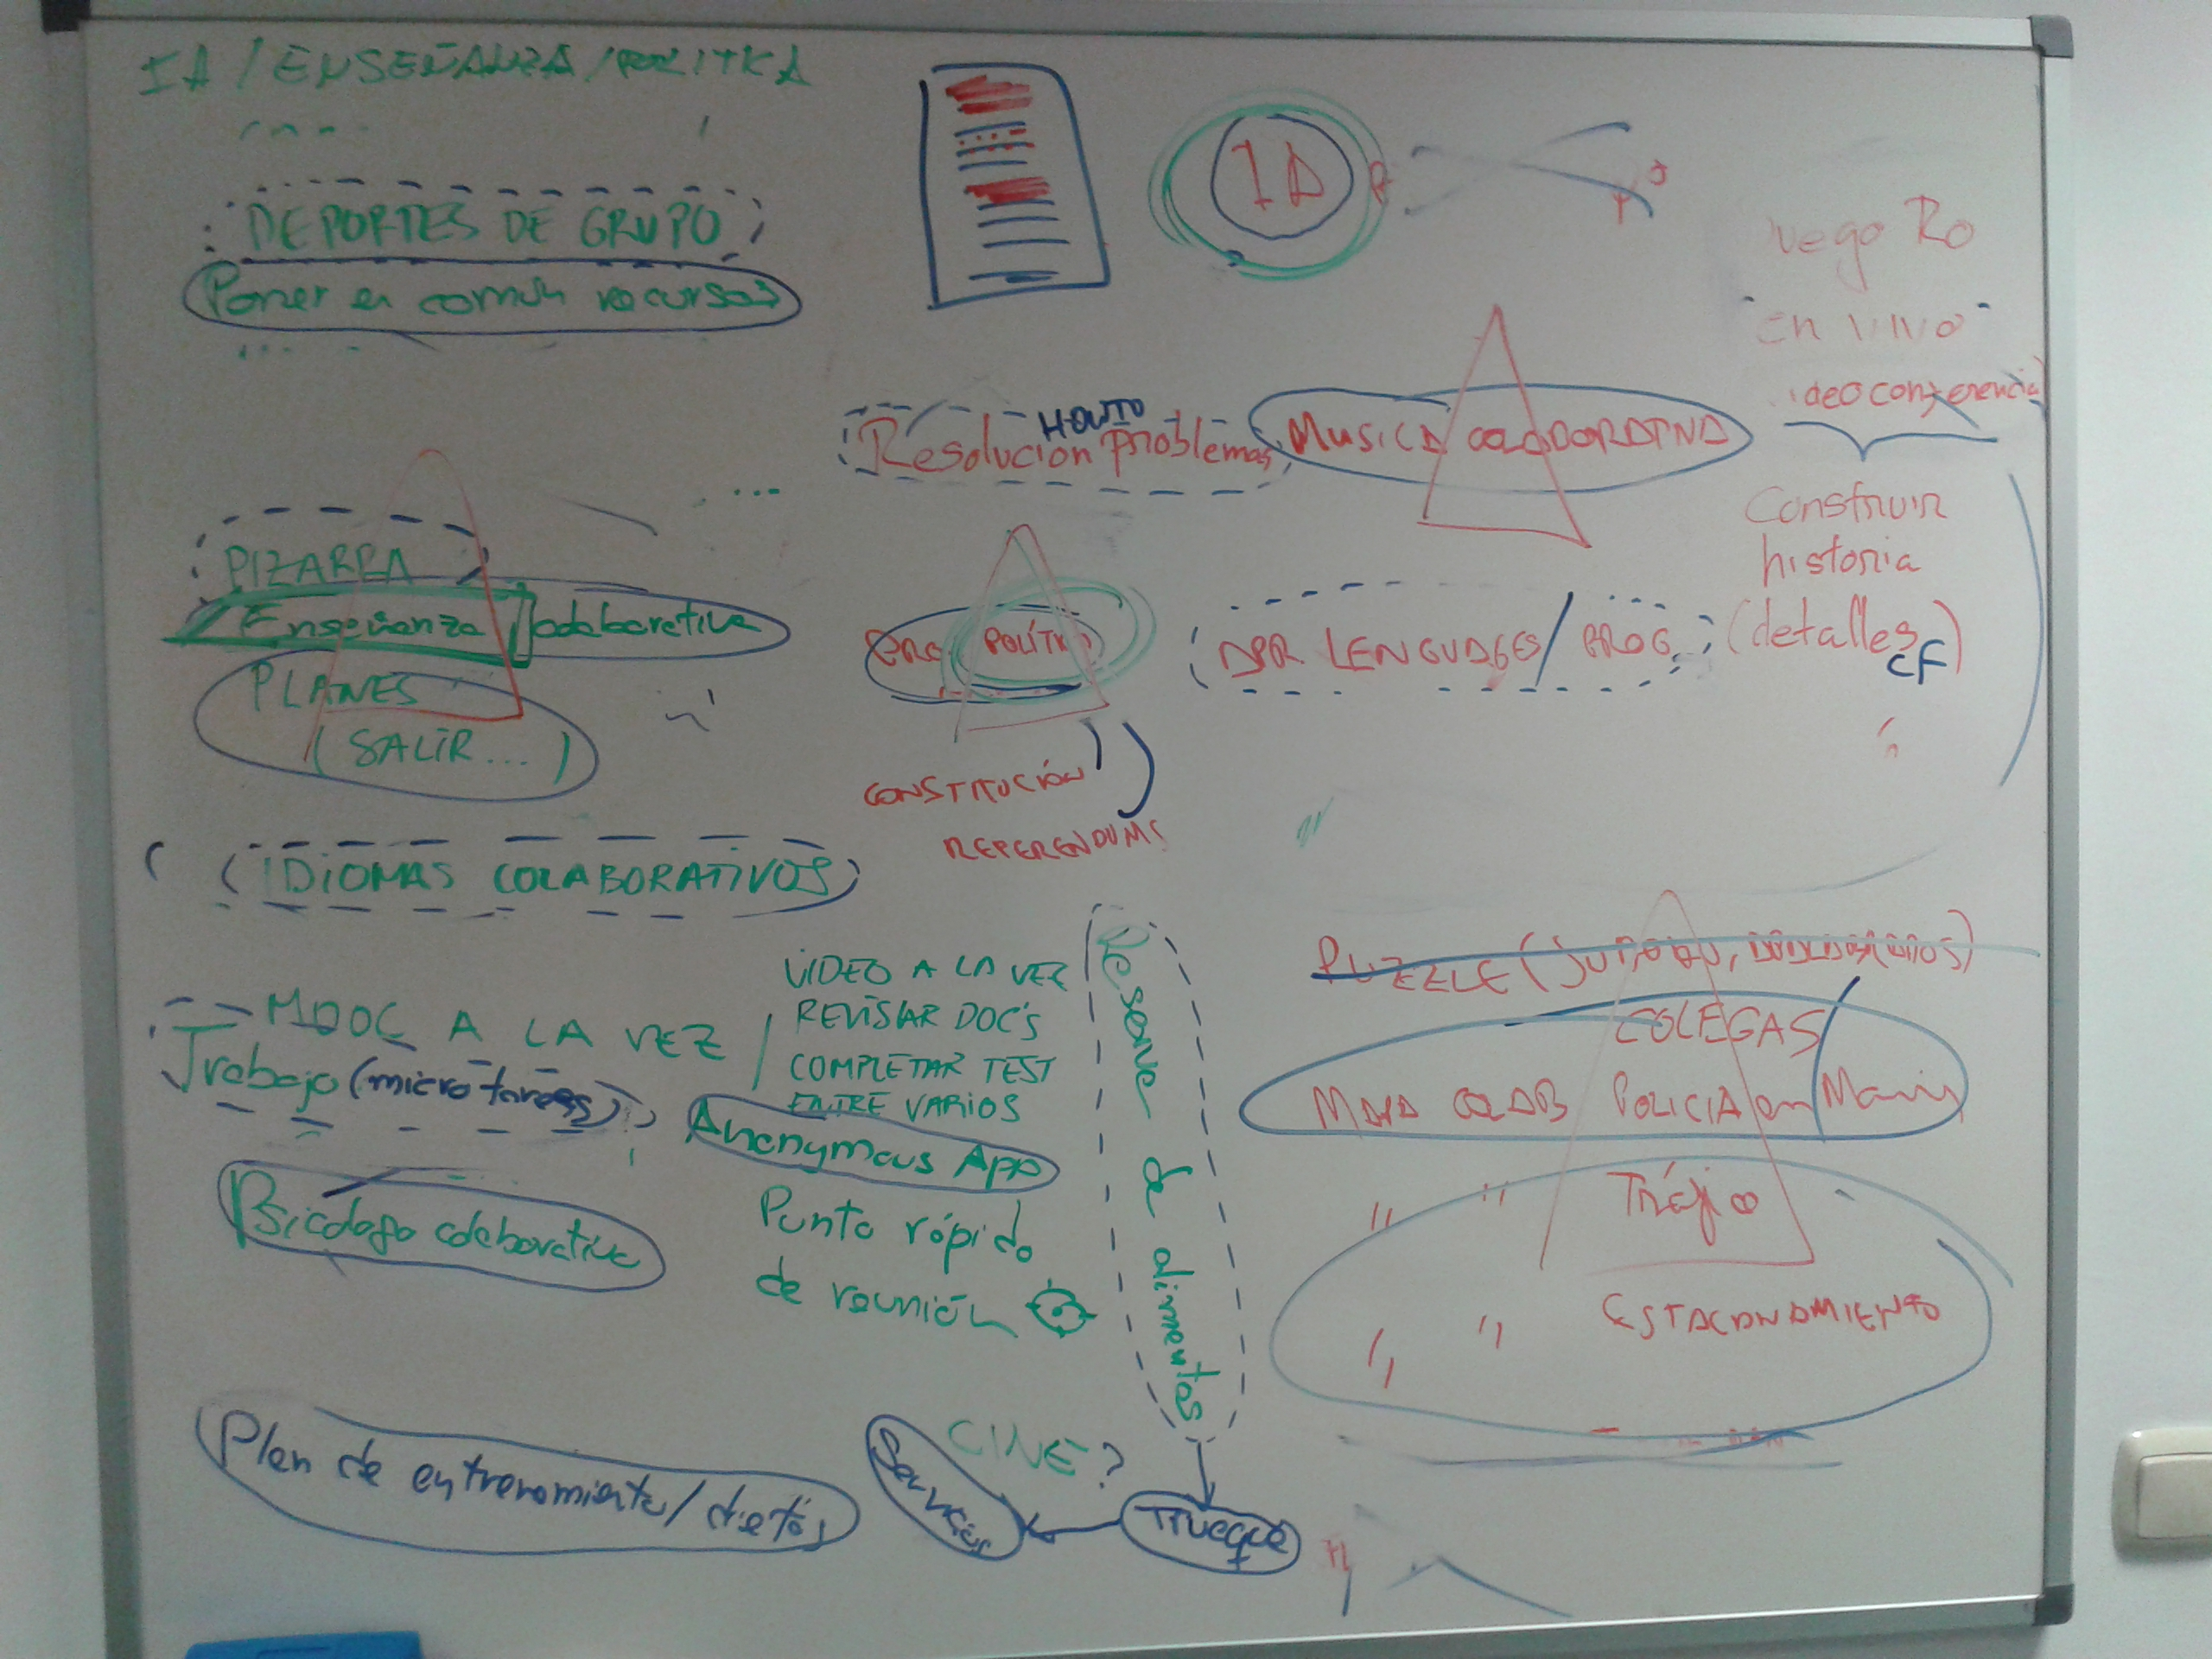
\includegraphics[keepaspectratio, scale=0.15]{Media/Captures/brainstorming.jpg}
      \caption{Brainstorming sobre la idea a desarrollar}
      \label{fig:brainstorming}
    \end{figure}
    
Con un gran repertorio de ideas expuestas sobre la sesión, descartamos aquellas que no nos motivaban llevarlas a cabo. Por lo que nos quedamos con tres ideas fundamentales a desarrollar en nuestra aplicación: Política, Música, Inteligencia Artificial y Mapas. Surgieron varias ideas colaborativas como desarrollar documentos políticos, programas electorales, comunicación entre colectivos en tiempo real, aprendizaje de música, edición de partituras y obras, aplicaciones colaborativas con inteligencia artificial, edición de mapas en tiempo real, lexicalización, etcétera.

Finalmente debido a intereses comunes, decimos realizar una aplicación colaborativa relacionado con el mundo de la política. Con el objetivo de que pudiera tener cierta repercusión y utilidad en las próximas citas electorales durante el año 2015. En esta aplicación podríamos recurrir a la edición de contenidos en tiempo real, ya fueran propuestas políticas, programas electorales y otro tipo de documentos. Como también hacer uso de alguna herramienta de Inteligencia Artificial para automatizar algunas tareas o realizar recomendaciones sociales.

\subsection{Adentrándonos en la idea}
La idea a desarrollar generada en una época dónde la política parecía haber despertado el interés de una parte considerable de la ciudadanía, podría ser una herramienta útil para participar en temas políticos que forma sencilla y atractiva. Dejando atrás los tópicos yo no entiendo de política, la política es aburrida, no sé a quién votar o no he leído nunca un programa electoral entre otros.

La herramienta ofrecería una nueva forma de participar en la política y de llevar a los ciudadanos los programas electorales ofertados por las diferentes formaciones políticas. De tal forma que los ciudadanos pudieran leer aquellos puntos de los programas más leídos, debatidos, comentados, etcétera. Así cualquier usuario tendría todos programas electorales en su bolsillo, por lo que no tendría que ir a la página web de cada formación política y descargarse un documento de 200 páginas. Pensamos que esta forma de presentar un programa político en un mundo donde las posibilidades de  comunicarnos se han desarrollado exponencialmente, no era la mejor manera de llegar a la mayor parte de la ciudadanía.

Por otra parte, la aplicación también debería ofrecer alguna herramienta donde realizar propuestas y debatirlas entre todos. De tal forma que tanto la ciudadanía como las formaciones políticas pudieran saber en cualquier momento cuáles son las principales preocupaciones de los ciudadanos y qué medidas o soluciones proponen para resolverlas.

Desde un primer punto de vista subjetivo, la aplicación quedó dividida en dos partes. Por un lado tendríamos los programas políticos que presentaran las formaciones políticas. Y por otro, todas las propuestas que elaboraran los ciudadanos individualmente o en colectivos sociales.

\subsection{Política en el mundo de la Informática}

\subsection{Democracia}

	\subsubsection{Democracia representativa}
	
	\subsubsection{Democracia participativa}
	
	\subsubsection{Democracia directa}
	
	\subsubsection{Democracia deliberativa}
	

\section{1ª Parte: Programas Políticos}
En esta sección se desarrollará en profundidad todo lo relacionado con los partidos políticos.

  \subsection{Estado del Arte}
En la actualidad no existe ningún tipo de aplicación orientada a debatir los programas electorales de los partidos políticos. Concretamente no hay ningún tipo de plataforma que agrupe los programas electorales de las diferentes candidaturas.
Lo más parecido que hemos podido encontrar han sido aplicaciones elaboradas por un partido político, orientada a dar a conocer su candidatura. En ella podremos ver la candidatura, vídeos y el programa electoral entre otros. Por ello pasamos a analizar las aplicaciones encontradas:

	\subsubsection{UPyD Parla}
La aplicación que presenta el candidato de UpyD Carlos Alt Bustelo para la alcaldía de Parla. Se trata de una alicación divulgativa donde podemos conocer todo lo esencial de la candidatura de UpyD para las elecciones del municiono de Parla en Mayo de 2015. Los candidatos, el programa, vídeos, etcétera.

	\begin{figure}[H]
      \centering
	
\includegraphics[keepaspectratio, scale=0.35]{Media/Captures/UPyDParla.png}
      \caption{UPyD Parla}
      \label{fig:upydparla}
    \end{figure}

	\subsubsection{$\sharp$RecuperaCórdoba}
De forma similar a la anterior, la candidatura de Pedro García a la provincia de Córdoba de Izquierda Unida, presenta su propuesta de gobierno de forma compacta. En la aplicación podremos encontrar la lista de los candidatos propuestos a la comunidad cordobesa, el programa electoral de la formación, las propuestas del partido, noticias de última hora y vídeos.

	\begin{figure}[H]
      \centering
	
\includegraphics[keepaspectratio, scale=0.35]{Media/Captures/IURecuperaCordoba.png}
      \caption{$\sharp$RecuperaCórdoba}
      \label{fig:recuperacordoba}
    \end{figure}
    
    	\subsubsection{PP Canarias}
    	
La delegación del Partido Popular en Canarias, presenta su aplicación móvil para promocionar a sus candidatos para las elecciones autonómicas y municipales de Mayo de 2015. La aplicación nos avisará de los eventos electorales, podremos consultar los candidatos, novedades, galería de imágenes y por su puesto el programa electoral.

	\begin{figure}[H]
      \centering
	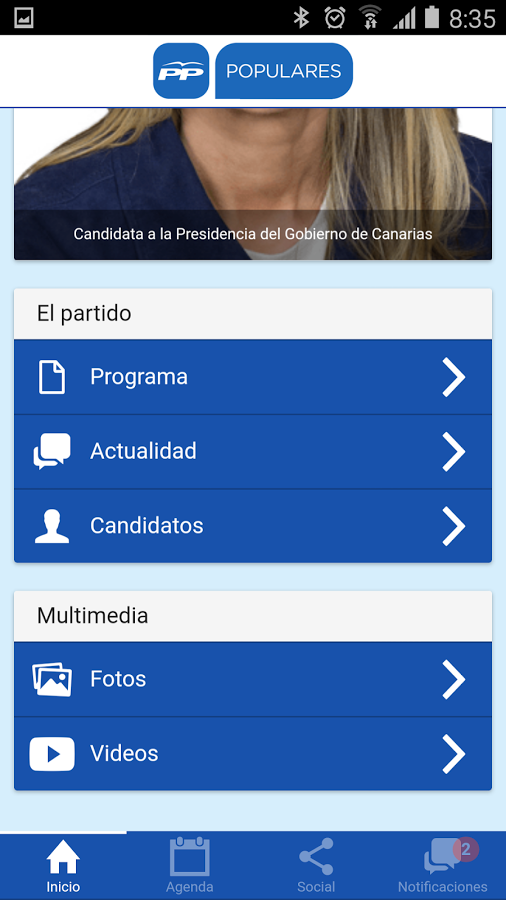
\includegraphics[keepaspectratio, scale=0.35]{Media/Captures/ppcanarias.png}
      \caption{PP Canarias}
      \label{fig:ppcanarias}
    \end{figure}

	\subsection{Intención}

La intención fundamental de la aplicación es llevar los programas electorales a los bolsillos de los ciudadanos. Vivimos en una sociedad digital, donde cada vez son más las personas que utilizan los teléfonos inteligentes para realizar todo tipo de tareas en su vida cotidiana.

En los últimos años las diferentes formaciones políticas han subido sus programas electorales a un documento en formato pdf que estaba disponible en su página web. Este documento generalmente extenso, no es un medio fácil de divulgar y mostrar a la ciudadanía. Por ello pensamos que una aplicación que pudiera visualizar las principales secciones de los programas políticos, podría ser especialmente útil para acercar los programas a los electores.

Llegando a crear un espacio donde poder informase sobre las distintas ofertas electorales, debatir las propuestas que propone cada formación política reducido en una aplicación que podremos consultar en cualquier momento.
  
	\subsection{Objetivos}
	
La aplicación pretende llevar las principales partes de los programas electorales de los partidos que se presenten a las elecciones. Por tanto, cualquier usuario podrá visualizar el apartado que desee consultar de cualquier partido político. Siendo esta la forma menos amigable de leerlo, se utilizarán distintas formas para compartir o divulgar determinadas secciones más populares.

Al inicio de la aplcación, mostrará una lista de las secciones de los programas más valoradas, más debatidas, peor valoradas e incluso las más incomprendidas. Por tanto creemos que puede ser una forma de acercar aquellas secciones más populares de forma más eficaz, al contrario que tener que consultar una determinada página dentro de un extenso pdf.

	\begin{figure}[H]
      \centering
	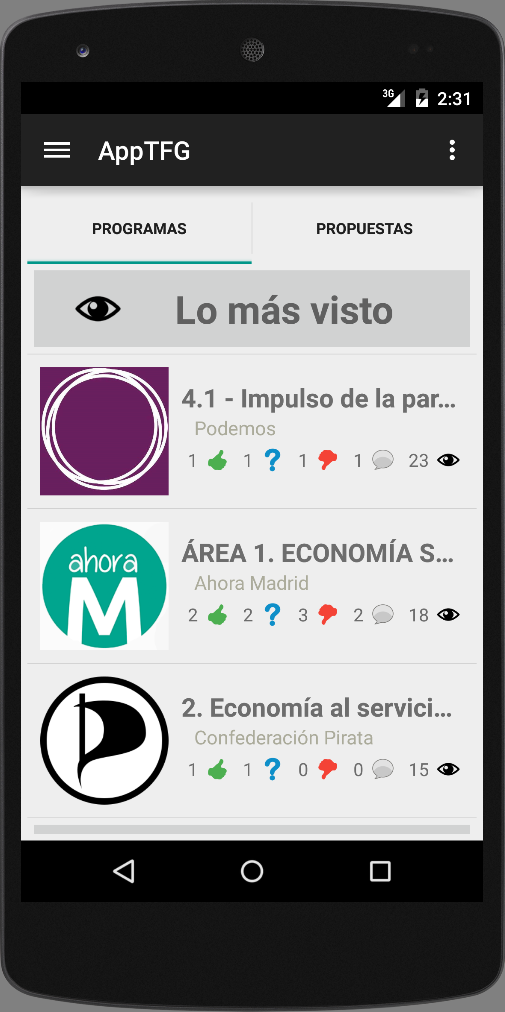
\includegraphics[keepaspectratio, scale=0.5]{Media/Captures/captTopSections.png}
      \caption{Vista principal de secciones}
      \label{fig:captTopSections}
    \end{figure}
    
Dentro de cada sección podemos visualizar el contenido de la sección a la que referencia el programa, y tendremos la opción de valorarla de forma positiva o negativa. También añadimos la posibilidad de indicar que no se ha entendido la sección. Pues a la hora de leer una propuesta de gobierno ubicada en una sección del programa, bien nos puede gustar, disgustar o simplemente no haber entendido la idea y por ello no votarla de forma positiva o negativa.

	\begin{figure}[H]
      \centering
	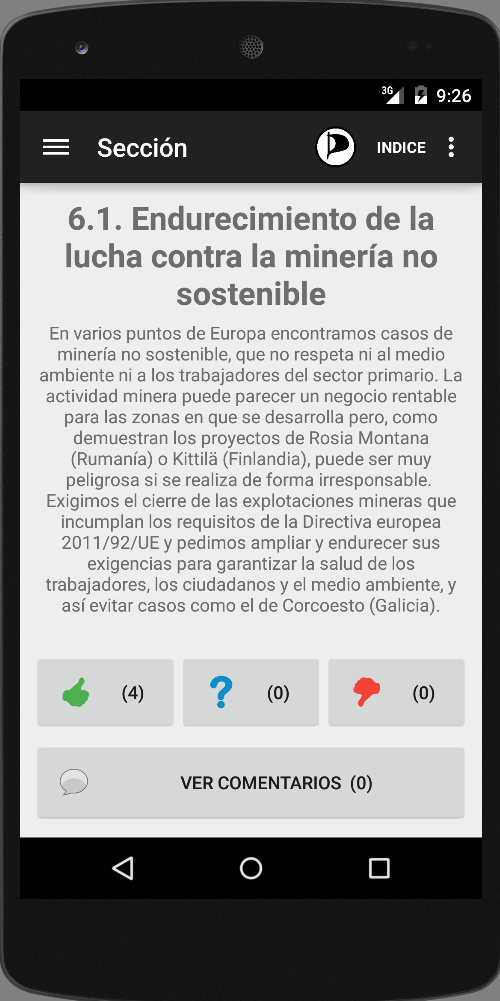
\includegraphics[keepaspectratio, scale=0.5]{Media/Captures/section.png}
      \caption{Visualizando una sección}
      \label{fig:captSection}
    \end{figure}
    
Sin olvidarnos de la parte social, en cada sección podemos hacer comentarios para intentar debatir las ideas fundamentales que propone la sección. O incluso hacer referencia a una determinada frase o párrafo.
	\subsection{Usabilidad}
	
	\subsection{Revisión de la aplicación}
Una vez que habíamos implementado todos los objetivos fundamentales de la aplicación, decidimos hacer una revisión para poner a prueba la aplicación. Para ello nos reunimos con un grupo de Labodemo \cite{ref:labodemo}, responsables del desarrollo de los portales de participación ciudadana del partido político Podemos \cite{ref:podemos} y la candidatura ciudadana de unidad popular Ahora Madrid \cite{ref:ahoramadrid}.

	\subsubsection{Reunión con Labodemo}
Tuvimos la oportunidad de establecer una conversación con dos miembros de Labodemo, en la que aprovechamos la oportunidad de mostrarles la aplicación que estábamos desarrollando. Ambos tenían experiencia en el desarrollo de plataformas de participación ciudadana en internet y nuevas tecnologías. Además fueron los responsables del desarrollo de los portales de participación del partido político Podemos y la candidatura ciudadana de unidad popular Ahora Madrid.

Limitarnos a mostrar las diferentes secciones de cada programa les resultó útil. Aunque no suficiente como para atraer a una cantidad considerable de usuarios. Antes de hablar con ellos, habíamos planteado desarrollar propuestas colaborativas en tiempo real aprovechando Wave. Pero no comprendieron la libertad de dar al usuarios la creación de propuestas colaborativas en tiempo real.

Dándole una vuelta al desarrollo de las propuestas de la aplicación, nos sugirieron que para atraer a usuarios a utilizar nuestra aplicación, deberíamos dejar cierta libertad a colectivos sociales. Por ejemplo, un grupo de animalistas debería tener un “espacio” en la aplicación donde poder crear sus propias propuestas, e incluso hacer comparativas personalizadas de lo que proponen los diferentes programas sobre los animales. Así surgirían propuestas y comparativas divididas por colectivos que abarcarían diferentes temáticas. Un usuario poco activo podría buscar un colectivo de profesores porque resulta ser su profesión, y ver las propuestas que se llevan a cabo o visualizar una comparativa respecto las medidas de educación de los diferentes programas políticos.

Organizar estas propuestas no sería tarea sencilla. En un principio se propuso como diferentes temas que puede tener un foro, en forma de post. Más tarde llegamos a la conclusión de que sería más cómodo para los colectivos dar la libertad de crear sus propios hilos, y en cada uno de ellos publicar las propuestas relacionadas con su colectivo.

Por último insistieron mucho en el tema de las comparativas. Sería de gran utilidad que la aplicación tuviera una parte de comparativas en la que los usuarios pudieran comparar los programas políticos en vez de leerlos sección por sección. Resultaría de gran interés a un autónomo visualizar las medidas que proponen los diferentes partidos políticos para los autónomos. Pero estas comparativas no podría realizarlas cualquiera, por lo que deberían realizarlas periodistas o expertos que hubieran realizado algún tipo de comparativa similar anteriormente. Nos sugirieron contactar con periodistas o colectivos que hubieran publicado algún tipo de comparativa en cuando a programas o medidas, para obtener algún tipo de ayuda o consejo a seguir.
	
	\subsubsection{Conclusión}

La reunión con dos de los miembros de Labodemo resultó de gran interés. Pues desde que decidimos la idea que íbamos a implementar, nunca habíamos puesto en práctica la aplicación o al menos no la habíamos verificado con el “mundo real”.

Los integrantes de Labodemo eran expertos en desarrollo de portales de participación ciudadana. Y sobre todo estaban muy familiarizados con el uso común que les suele dar la gente a este tipo de aplicación. Por lo que sabían determinar las claves para que una aplicación tuviera un movimiento considerable de usuarios desde el comienzo.

El tema de visualizar los programas políticos no les gustó demasiado. Expusieron que un ciudadano de a pie, no iba a molestarse en leer los programas políticos. Bien porque no los entienda o porque les resulte aburridos. Ellos argumentaban que los colectivos sociales serían los usuarios más activos en nuestra aplicación, por lo que debíamos enfocar más el desarrollo hacia la partición ciudadana y el uso de propuestas o comparativas por colectivo.

Tras esta reunión decidimos replantear la aplicación en base a los consejos que obtuvimos con la reunión de Labodemo. Incluimos las propuestas como parte de nuestra aplicación y empezamos a pensar la forma de colaborar de grupos y colectivos. También intentamos contactar con colectivos y personas interesadas en el desarrollo de la aplicación. Finalmente, conseguimos concretar una entrevista con Javier de la Cueva \cite{ref:jdelacueva}.
	
	\subsubsection{Reunión con Javier de la Cueva}
	
	\subsubsection{Conclusión}

  
\section{2ª Parte: Propuestas y Categorización}
  \subsection{Estado del Arte}

  \subsection{Intención}
  \subsection{Objetivos}
  \subsection{Usabilidad}
  
\section{3ª Parte: Encuestas de intención de voto}
  \subsection{Estado del Arte}

  \subsection{Intención}
  \subsection{Objetivos}
  \subsection{Usabilidad}
  
  
\section{Tecnologias y Metodologías de la app}

  \subsection{Arquitectura de la aplicacción}
  
La arquitectura está compuesta por tres módulos principales de los que hablaremos en profundidad en las siguientes subsecciones. Como cliente móvil tendremos la aplicación desarrollada en Android, que realizará peticiones HTTP al servicio web alojado en OpenShift, una plataforma que permite alojar servicios web de forma gratuita. Dentro del servicio contaremos con una API RESTful que será quien gestione las peticiones de la aplicación móvil mediante el protocolo HTTP.

	\begin{figure}[H]
      \centering
	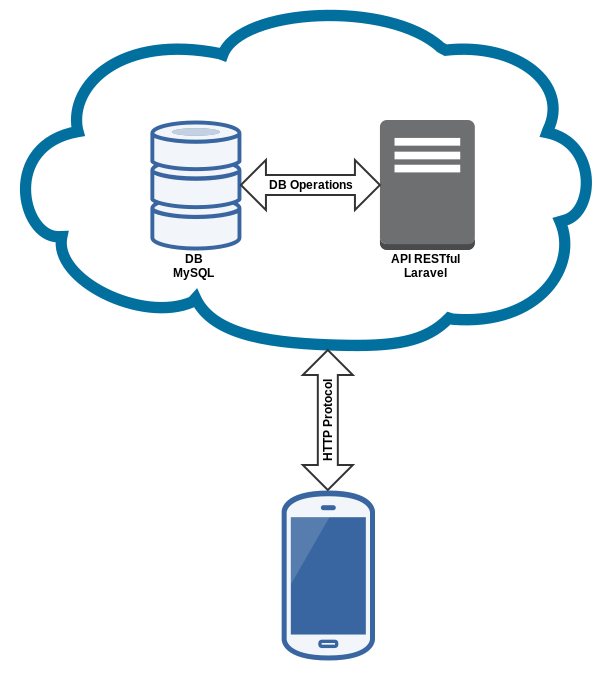
\includegraphics[keepaspectratio, scale=0.4]{Media/Captures/architecture.png}
      \caption{Arquitectura de la aplicacción.}
      \label{fig:architecture}
    \end{figure}

Por último, la base de datos MySQL alojada en el servidor de OpenShift \cite{ref:OpenShift}, almacenará toda la información relacionada con la aplicación. La API RESTful será quien gestione las operaciones de la base de datos.

	\subsection{Back-end}

  		\subsubsection{Base de Datos}\label{sssec:database}
Para la implementación de la base de datos, se ha utilizado un modelo relacional para la definición de las tablas. Utilizando MySQL \cite{ref:MySQL} como sistema de gestión de base de datos phpMyAdmin \cite{ref:phpMyAdmin} como herramienta de gestión gráfica de la base de datos.

La base de datos está formada por un total de 12 tablas donde se almacena toda la información relacionada con los programas de los partidos políticos, las propuestas ciudadanas, encuestas, comparativas, …, y otros datos más técnicos como la gestión de los usuarios, la relación de los comentarios o la relación entre las secciones y comparativas entre otras.

	\begin{figure}[H]
      \centering
	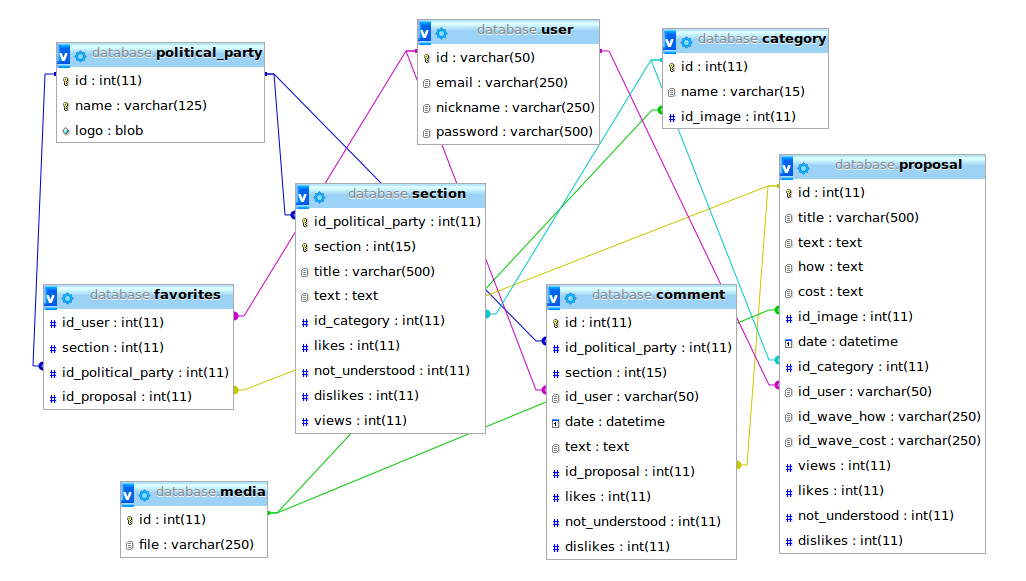
\includegraphics[keepaspectratio, scale=0.30]{Media/Captures/database.png}
      \caption{Modelo entidad-relación de la base de datos.}
      \label{fig:ermodel}
    \end{figure}
    
Las tablas section y \textit{political-party} son utilizadas para guardar información estática en la aplicación. Es decir, en la tabla \textit{political-party} se almacenan los partidos políticos que se presentan a unas elecciones, y en la tabla \textit{section}, las diferentes secciones de un programa electoral. Tan sólo modificaremos las columnas de \textit{likes}, \textit{dislikes}, \textit{not-understood} y \textit{views} para obtener estadísticas de uso de cada sección. El resto de las columnas permanecerán intactas.

Las demás tablas serán utilizadas para guardar datos dinámicos en la aplicación. Datos que normalmente genera un usuario visitando una sección de un programa, creando una propusta, haciendo un comentario, etc.

    
		\subsubsection{Service REST}\label{sssec:rest}
		
Para establecer la conexión de la base de datos con la aplicación desarrollada en Android, hemos utilizado Laravel como servicio web. Laravel \cite{ref:laravel}  un framework de código abierto para desarrollar aplicaciones web con PHP 5.

Laravel nos permite montar un sistema de RESTful para que el cliente móvil pueda hacer peticiones al servicio web. Estas peticiones se realizan mediante el protocolo HTTP, en función de la operación que deseemos hacer, haremos una petición GET, POST, PUT, …, etcétera.

	\begin{figure}[H]
      \centering
	
\includegraphics[keepaspectratio, scale=0.30]{Media/Captures/laravel5.png}
      \caption{Pantalla principal de Laravel 5.}
      \label{fig:laravel5}
    \end{figure}

Establecer un servicio RESTful nos proporciona una gran flexibilidad. Pues no solo podremos hacer peticiones desde el cliente en Android, si no que más adelante si pretendemos desarrollar una versión web o incluso un cliente para iOS, las peticiones serán las mismas.

Para organizar las diferentes peticiones en función de su uso y requisitos, Laravel permite montar una API REST (Representational State Transfer), un estilo de arquitectura software para sistemas hipermedia distribuidos como la World Wide Web. Este término se originó en una tesis doctoral sobre la web escrita por Roy Fielding \cite{ref:RESTPhd}.

  \subsection{Frontend}

\newpage
\thispagestyle{sectioned}
\chapter{Estado del Arte}

\section{Wave: Wave In A Box (WIAB)}\label{sec:wiab}
	    
	Wave In a Box (WIAB) \cite{ref:wave_in_a_box} es el código fuente liberado por Google y completado por la comunidad de Apache tras pasar el proyecto a sus manos en el año 2012. Al igual que el resto del código de la tecnología que heredó de Google, está implementado en Java usando OpenJDK \cite{ref:openjdk}. La instalación trae consigo un cliente web desarrollado en Java usando el framework Google Web Toolkit (GWT) \cite{ref:gwt}, lo que genera código JavaScript ejecutable en el navegador. Este cliente web sirve como prueba de concepto de las funcionalidades básicas del Modelo Conversacional de Wave, pudiendo gesionar waves, usuarios y extensiones. Actualmente cualquiera puede descargar y desplegar WIAB en su ordenador siguiendo los pasos que nos proporcionan en su wiki \cite{ref:wave_in_a_box_wiki}. La aplicación se distribuye en forma de código fuente, accesible entre otras formas desde su repositorio de GitHub \cite{ref:wave_in_a_box_github}. Existen asimismo servidores de prueba ya desplegados en Internet sobre los que se puede observar el funcionamiento de WIAB \cite{ref:wave_in_a_box_server}.
   		
	\begin{figure}[H]
      \centering
		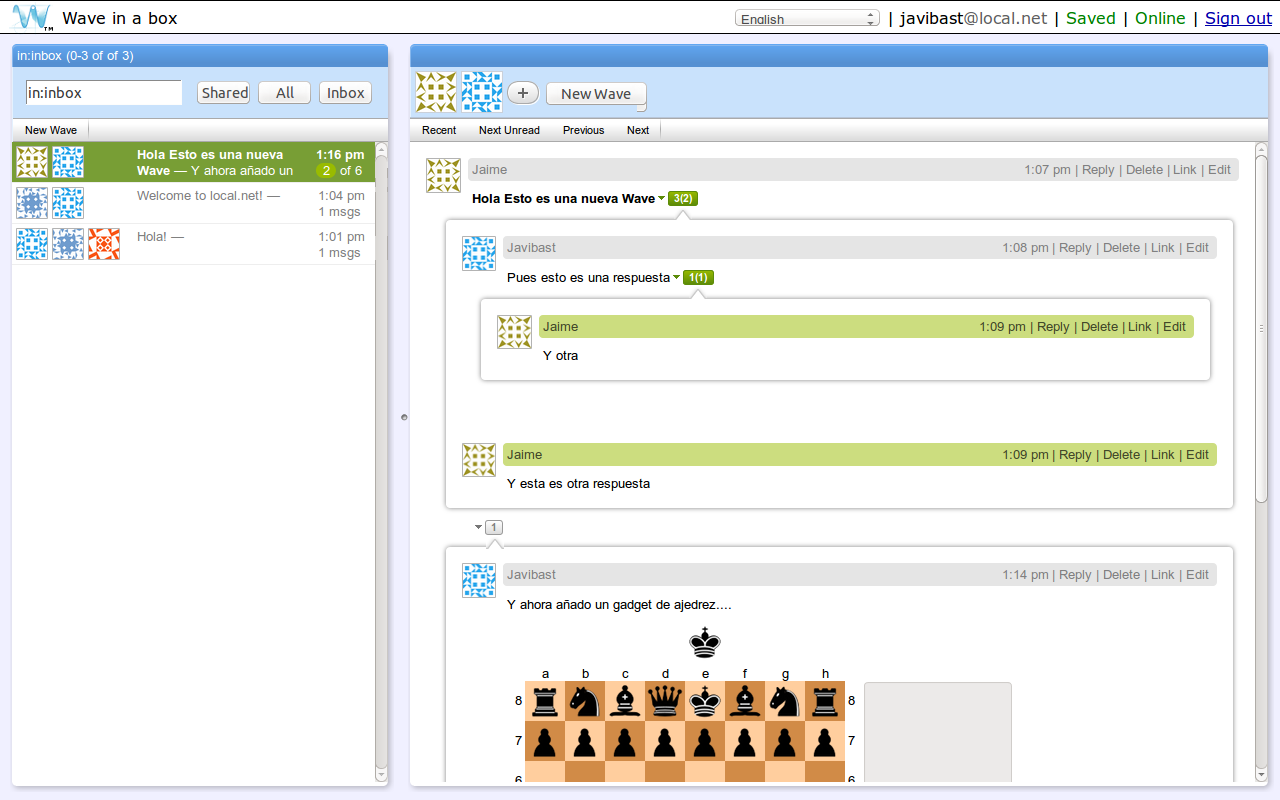
\includegraphics[keepaspectratio, scale=0.3]{Media/Captures/WIAB_Server.png}
      \caption{Cliente Wave In A Box}
      \label{fig:wiab_client}
    \end{figure} 

\section{Edición Colaborativa en Tiempo Real}

En esta sección veremos algunas de las soluciones disponibles actualmente que, al igual que Wave, permiten editar contenido de forma colaborativa y en tiempo real. Este contenido puede ser muy variado, aunque lo más usual suele ser proporcionar edición de texto en tiempo real mediante el uso de Transformaciones Operacionales (OT) \cite{ref:how_ot_works}. Sin embargo, todas estas plataformas utilizan una arquitectura de servidor centralizado para ofrecer estas funcionalidades, mientras que Wave utiliza una arquitectura federada en la que no existe un servidor central (Ver Sección \ref{sssec:federation}).

De esta manera, primero veremos las principales herramientas de desarrollo (APIs) más utilizadas actualmente, para después pasar a ver algunas de las plataformas que hacen uso de esta tecnología. En su mayoría son para web, aunque existen unas pocas para Android. 
	
	\subsection{APIs Centralizadas}
	
	La mayor parte del desarrollo de tecnologías de Colaboración en Tiempo Real (RTC) se realiza mediante APIs que son propiedad de determinadas compañias y que no utilizan una arquitectura federada, sino que toda la información pasa por un servidor central que controla el RTC. A continuación veremos algunas de las más utilizadas hoy en día.
	
	\subsubsection{Google Realtime API}\label{sssec:googleAPI}
	
	Google Realtime API \cite{ref:google_api} permite construir aplicaciones de colaboración en tiempo real utilizando la tecnología de Transformaciones Operacionales (OT) presente en Google Docs. Utiliza JavaScript para poder construir construir en nuestro cliente web un modelo de datos (\textit{Realtime Data Model}) que se guarda en sus servidores y gestiona automaticamente los cambios realizados por cualquiera de los usuarios que colaboran en tiempo real. Estos cambios en el modelo son notificados al servidor y al resto de usuarios mediante eventos que se lanzan al modificar los datos sobre los que se está colaborando. Para utilizarlo es necesario tener cuenta en la Consola de Desarrolladores de Google y activar el uso de esta API con nuestras credenciales de usuario. Existe asimismo una versión (privativa) de esta API compatible con Android.
	
	\subsubsection{Microsoft RTC Client API}
	
	Microsoft RTC Client API	 \cite{ref:microsoft_api} permite construir aplicaciones que permitan realizar llamadas de audio/video o sesiones de mensajería instantánea (IM) de texto por Internet y en tiempo real. Las aplicaciones se deben escribir en C++ o Visual Basic y pueden ser utilizadas tanto en PC como en dispositivos móviles siempre que ejecuten un sistema operativo Windows.
	
	\subsubsection{WebRTC}
	
	WebRTC \cite{ref:webRTC} (Web Real-Time Communication) es un API open-source (bajo licencia BSD) actualmente en desarrollo por Google y la World Wide Web Consortium (W3C) y que pretende dotar a los navegadores web de capacidades de comnicación en tiempo real entre sí sin necesidad de plugins externos. En la actualidad se encuentra en su versión 1.0 y soporta los navegadores Firefox y Chrome. 
	
	
	\subsubsection{Mozilla TogetherJS}

	Mozilla TogetherJS \cite{ref:togetherjs_api} es una librería gratuita y de código libre (bajo licencia pública Mozilla v2) que permite añadir capacidades de colaboración en tiempo real a una página web. Utiliza WebRTC y webSockets para establecer comunicaciones peer-to-peer (P2P) entre dos o más navegadores Web. No proporciona alamcenamiento persistente de los datos y es necesario tener un Servidor que establezca la conexión. Con esta herramienta se puede editar texto en tiempo real (usando Transformaciones Operacionales), establecer chats de audio/video y sincronizar el contenido de los navegadores. Está disponible en \textit{GitHub} \cite{ref:github} para contribuir a su desarrollo. 	
	
	\subsubsection{ShareJS}

	ShareJS \cite{ref:shareJS} es una plataforma open-source (bajo licencia MIT) que dispone de un pequeño servidor basado en Node.js y una librería de cliente JavaScript que permiten la edición colaborativa de contenido mediante Transformaciones Operacionales. Permite actuar sobre objetos JSON o sobre texto plano. Está disponible en \textit{GitHub} para scontribuir a su desarrollo.
	
	\subsubsection{Goodow}
	
	Goodow \cite{ref:goodow} es un framework open-source de reciente desarrollo que proporciona un API muy similar a \textit{Google Real-Time API} (Ver Sección \ref{sssec:googleAPI}) para colaboración en tiempo real mediante el uso de Transformaciones Operacionales. Dispone asimismo de dos clientes básicos para Android e iOS, utilizando una implementación del Servidor propia.	
	
	\subsection{Plataformas Web y Android}

	En las siguientes secciones veremos algunas de las plataformas Web y Android que hacen uso de tecnologías de Colaboración en Tiempo Real.	
	
	\subsubsection{Google Docs}
	
	Google Docs \cite{ref:google_docs} es la plataforma de Google para edición de documentos de forma colaborativa y en Tiempo Real usando su API Realtime (Ver Sección \ref{sssec:googleAPI}). Permite que varios usuarios con cuenta de Google creen y editen colaborativamente un documento a la vez. Puedes ver los cursores de cada usuario e interactuar con ellos mediante un chat. También permite escribir sugerencias a modo de notas en el margen sobre lo ya escrito. Dispone de versión web y móvil, pudiendo interactuar entre ellas sin problemas.
	
	\begin{figure}[H]
        \centering
        \begin{subfigure}[b]{0.6\textwidth}
                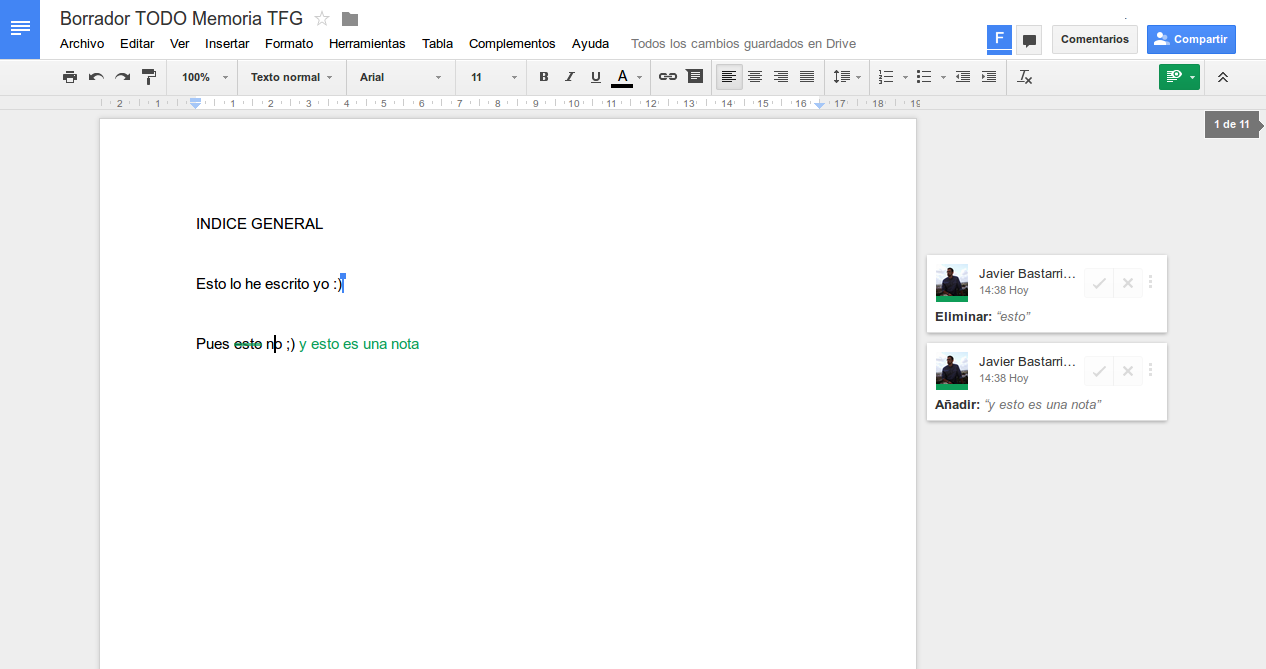
\includegraphics[width=\textwidth, height=6cm]{Media/Captures/googleDocsWeb.png}
                \caption{Interfaz Web}
                \label{fig:googleDocsWeb}
        \end{subfigure}
        ~
        \begin{subfigure}[b]{0.3\textwidth}
                
\includegraphics[width=\textwidth, height=7cm]{Media/Captures/googleDocsApp.jpg}
                \caption{Interfaz Android}
                \label{fig:googleDocsApp}
        \end{subfigure}
        \caption{Capturas de Google Docs}\label{fig:googleDocsCaptures}
	\end{figure}
	
	\subsubsection{Etherpad}
	
	Etherpad \cite{ref:etherpad} es un editor colaborativo en tiempo real open-source (bajo licencia Apache 2.0). Permite a varios autores editar a la vez un mismo documento de texto, resaltando en distintos colores lo editado por cada persona y con la opción de un chat para comunicarse entre sí. Existen múltiples servicios que hacen uso de este editor, siendo uno de las más conocidas TitanPad \cite{ref:titanpad}.
	
	\begin{figure}[H]
		\centering
			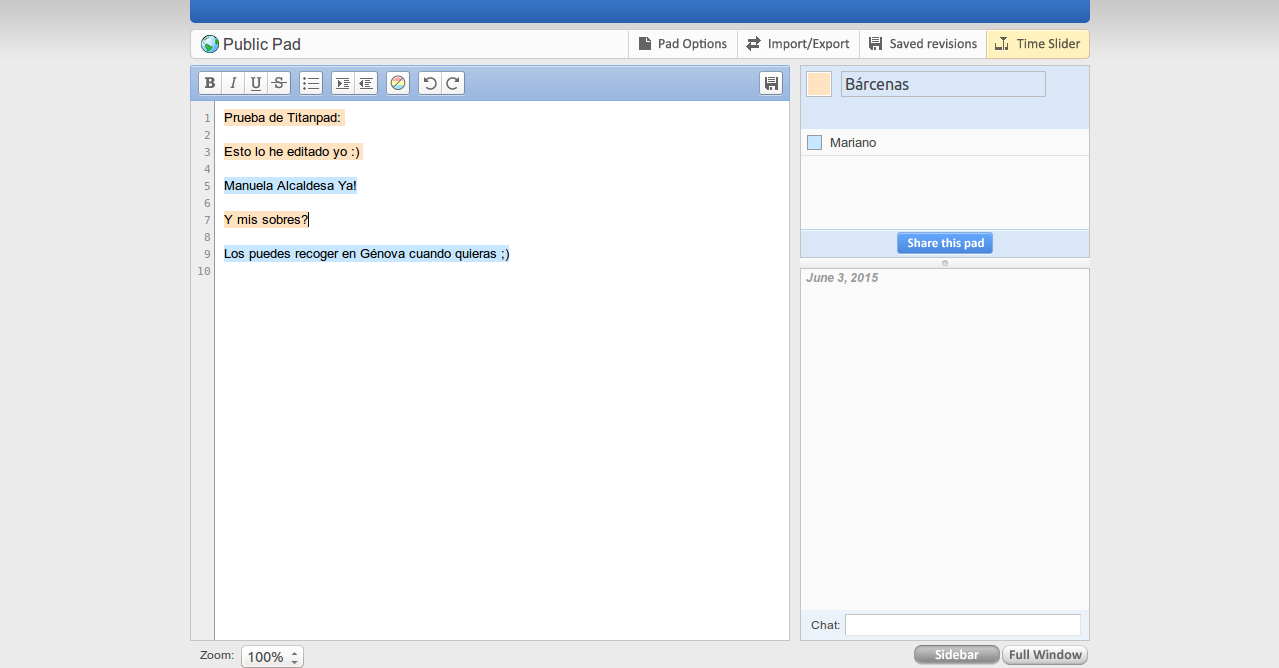
\includegraphics[keepaspectratio, scale=0.30]{Media/Captures/titanpadWeb.png}
		\caption{Captura de TitanPad: Ejemplo de uso de EtherPad}
		\label{fig:titanpad}
	\end{figure} 	
	
	\subsubsection{Colorillo}
	
	Colorillo \cite{ref:colorillo} es una aplicación web básica de dibujo colaborativo en tiempo real. Cualquier usuario puede empezar a dibujar sobre un nuevo lienzo en blanco con diversos colores y compartir este lienzo con otros usuarios para dibujar entre todos. De cada usuario podemos ver su procedencia aproximada sobre un mapa y el color que actualmente está utilizando. Existe también opción para chatear con otros usuarios. Los dibujos se pueden descargar y tienen todos licencia Creative Commons BY 3.0.
	
	\begin{figure}[H]
		\centering
			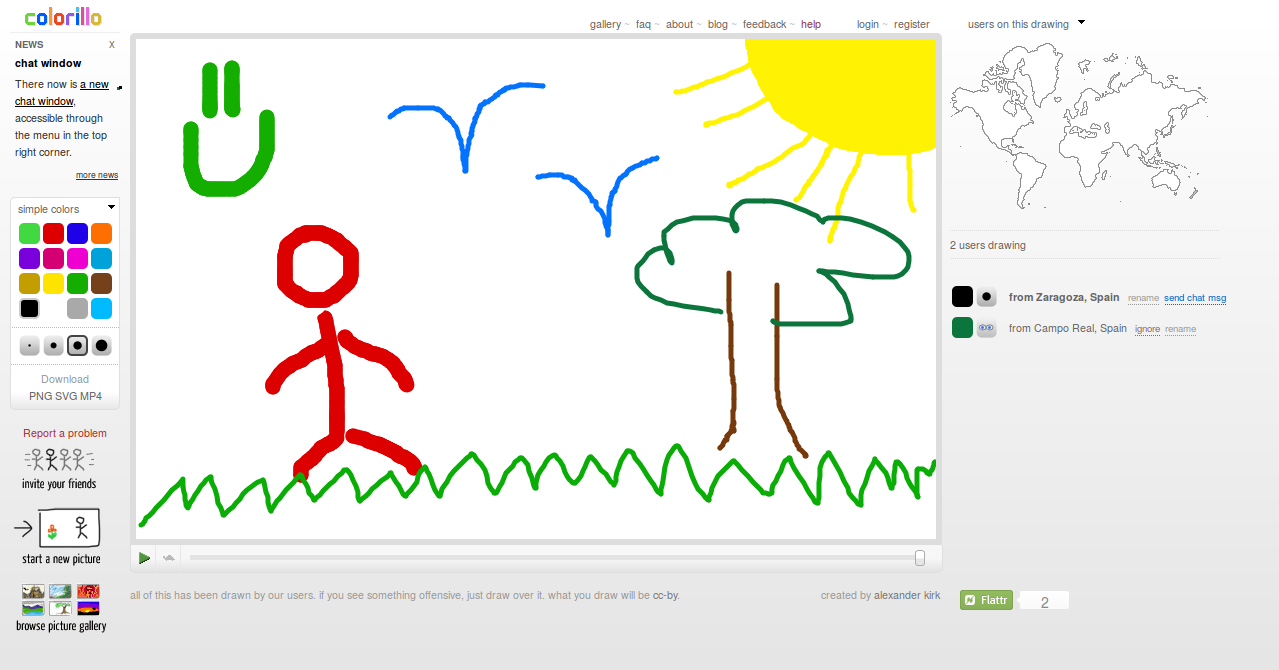
\includegraphics[keepaspectratio, scale=0.30]{Media/Captures/colorilloWeb.png}
		\caption{Captura de Colorillo}
		\label{fig:colorillo}
	\end{figure}  	
	
	\subsubsection{ShareLaTeX}
	
	ShareLaTeX \cite{ref:shareLatex} es un editor web colaborativo de documentos escritos en LaTeX en tiempo real. Permite elaborar documentos LaTeX entre varias personas, ofreciendo una interfaz que incluye una previsualización del resultado en PDF. Desde 2014 es open-source (bajo licencia AGPL v3) y cualquiera puede descargarselo de \textit{GitHub} e instalar su propio servidor (escrito en Node.js) de ShareLaTeX. En su web ofrecen también opciones de pago con extras como un control de versiones o sincronización con Dropbox.
	
	\begin{figure}[H]
		\centering
			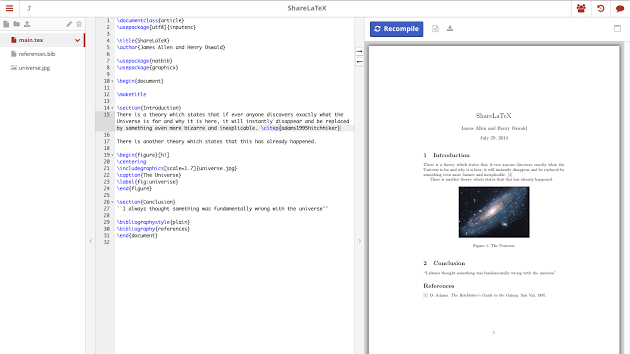
\includegraphics[keepaspectratio, scale=0.60]{Media/Captures/shareLatexWeb.png}
		\caption{Captura de ShareLaTeX}
		\label{fig:shareLaTeX}
	\end{figure}  
		
	\subsubsection{Samepage}
	
	Samepage \cite{ref:samepage} es una aplicación, tanto para web como para plataformas móviles (Android e iOS), que permite crear documentos que pueden ser editados de forma colaborativa y en tiempo real por múltiples usuarios. Para ello es necesario solo es tener una cuenta de samepage. Tanto el cliente web como el móvil permiten interactuar entre ellos para crear nuevas páginas, editar texto y hacer comentarios, aunque la versión web permite también añadir tablas, imágenes y archivos.
	
	\begin{figure}[H]
        \centering
        \begin{subfigure}[b]{0.6\textwidth}
                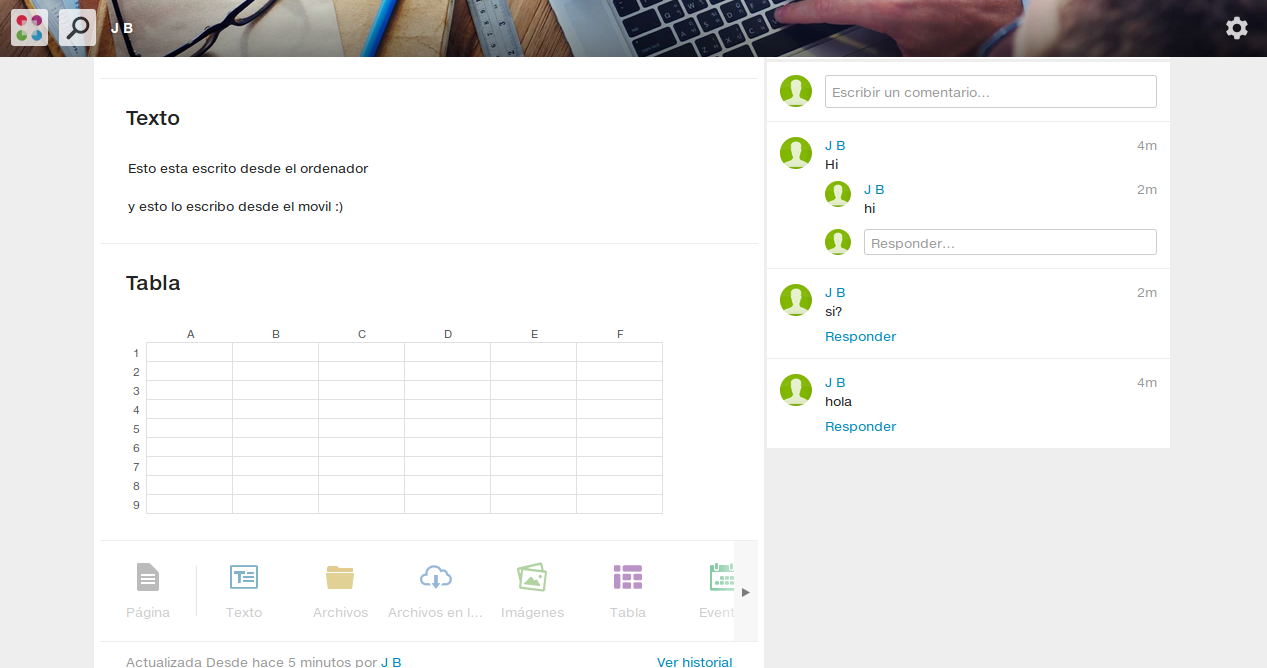
\includegraphics[width=\textwidth, height=6cm]{Media/Captures/samepageWeb.png}
                \caption{Interfaz Web}
                \label{fig:samepageWeb}
        \end{subfigure}
        ~
        \begin{subfigure}[b]{0.3\textwidth}
                
\includegraphics[width=\textwidth, height=7cm]{Media/Captures/samepageApp.jpg}
                \caption{Interfaz Android}
                \label{fig:samepageApp}
        \end{subfigure}
        \caption{Capturas de Samepage}\label{fig:samepageCaptures}
	\end{figure}
	
	
	\subsubsection{Quip}
	
	Quip \cite{ref:quip} es una aplicación para dispositivos móviles (Android e iOS) desarrollada con el objetivo de aumentar la productividad en los trabajos en grupo. Permite elaborar documentos, hojas de cálculo y listas de tareas compartidas y editables de forma colaborativa en tiempo real, pudiendo realizar también comentarios sobre ellas. Dispone también de una versión web, pero es necesario tener cuenta para usarla.
	
	\begin{figure}[H]
        \centering
        \begin{subfigure}[b]{0.3\textwidth}
                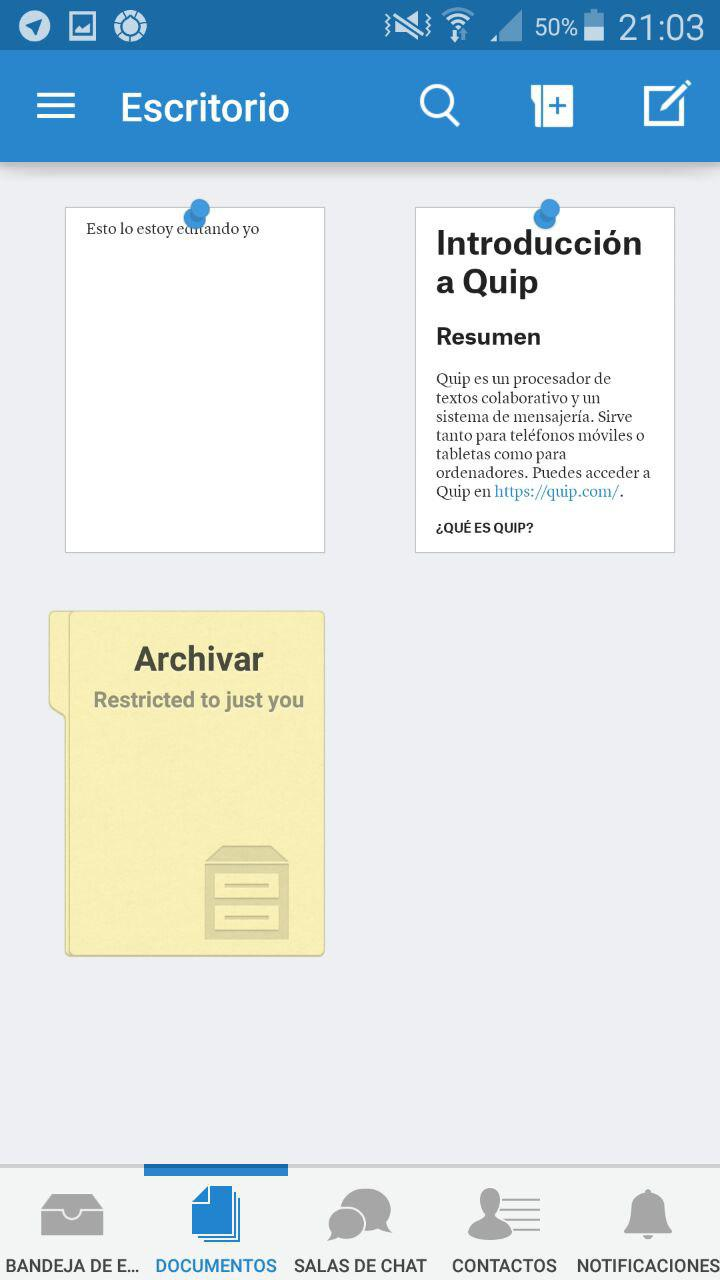
\includegraphics[width=\textwidth]{Media/Captures/quipDesktop.jpg}
                \caption{Escritorio}
                \label{fig:quipDesktop}
        \end{subfigure}
        ~
        \begin{subfigure}[b]{0.3\textwidth}
                
\includegraphics[width=\textwidth]{Media/Captures/quipEdit.jpg}
                \caption{Edición de texto}
                \label{fig:quipText}
        \end{subfigure}
        ~
        \begin{subfigure}[b]{0.3\textwidth}
                
\includegraphics[width=\textwidth]{Media/Captures/quipComment.jpg}
                \caption{Comentarios}
                \label{fig:quipComments}
        \end{subfigure}
        \caption{Capturas de Quip}\label{fig:quipCaptures}
	\end{figure}
	
	

\section{Aplicación Android: DemoCritics}

En esta sección exploraremos algunas de las principales aplicaciones informáticas que existen en la actualidad destinadas a la participación ciudadana en propuestas, lectura de programas electorales o divulgación de candidaturas.

\subsection{Programas Políticos}

En la actualidad no existe ningún tipo de aplicación móvil orientada a debatir los programas electorales de los partidos políticos en su conjunto. Concretamente no existe ningún tipo de plataforma que agrupe en un solo sitio los programas electorales de las diferentes candidaturas.
Lo más parecido que hemos podido encontrar han sido aplicaciones elaboradas por un partido político, orientadas a dar a conocer su candidatura. En ellas podemos ver normalmente, entre otros, la presentación de la candidatura, vídeos propagandísticos y el programa electoral. 

Pasamos ahora a analizar algunas de las aplicaciones móviles encontradas, identificando en cada caso aspectos e ideas que nos han resultado positivos y negativos.

\subsubsection{UPyD Parla}
La aplicación presenta al candidato de UpyD Carlos Alt Bustelo para la alcaldía de Parla. Se trata de una alicación divulgativa donde podemos conocer todo lo esencial de la candidatura de UpyD para las elecciones del municipio de Parla en Mayo de 2015: los candidatos, el programa, vídeos, etc.

\begin{figure}[H]
        \centering
        \begin{subfigure}[b]{0.3\textwidth}
                
\includegraphics[width=\textwidth]{Media/Captures/UPyDParlaIndex.jpg}
                \caption{Indice Programa}
                \label{fig:upydIndex}
        \end{subfigure}
        ~
        \begin{subfigure}[b]{0.3\textwidth}
                
\includegraphics[width=\textwidth]{Media/Captures/UPyDParlaSection.jpg}
                \caption{Sección Programa}
                \label{fig:upydSection}
        \end{subfigure}
        ~
        \begin{subfigure}[b]{0.3\textwidth}
                
\includegraphics[width=\textwidth]{Media/Captures/UPyDParlaCandidates.jpg}
                \caption{Candidatos}
                \label{fig:upydCandidates}
        \end{subfigure}
        \caption{Capturas de UPyD Parla}\label{fig:upydCaptures}
\end{figure}

 - \underline{Aspectos positivos}:

\begin{itemize}
	\item Presentación de Programa Electoral estructurado con Indice inicial.
	\item El Programa se lee dentro de la app, no nos lleva a leer el programa en PDF de la web. 
	\item Presentación de una Sección del Programa Electoral de forma resumida, teniendo la opción de leer la sección entera al pulsar un botón.
\end{itemize}

 - \underline{Aspectos negativos}:

\begin{itemize}
	\item Posee una sección llamada ''Memes'' cuyo nombre no se entiende ya que se limita a mostrar carteles propagandísticos de la candidatura. 
\end{itemize}

\subsubsection{$\sharp$RecuperaCórdoba}
Esta app presenta la candidatura de Pedro García de Izquierda Unida a la provincia de Córdoba, informando de su propuesta de gobierno de forma resumida. En la aplicación podremos encontrar la lista de los candidatos propuestos a la comunidad cordobesa, el programa electoral de la formación, las propuestas del partido, noticias de última hora y vídeos.

\begin{figure}[H]
        \centering
        \begin{subfigure}[b]{0.3\textwidth}
                
\includegraphics[width=\textwidth]{Media/Captures/IURecuperaCordoba.jpg}
                \caption{Indice Programa}
                \label{fig:iuIndex}
        \end{subfigure}
        ~
        \begin{subfigure}[b]{0.3\textwidth}
                
\includegraphics[width=\textwidth]{Media/Captures/IURecuperaCordobaSection.jpg}
                \caption{Sección Programa}
                \label{fig:iuSection}
        \end{subfigure}
        ~
        \begin{subfigure}[b]{0.3\textwidth}
                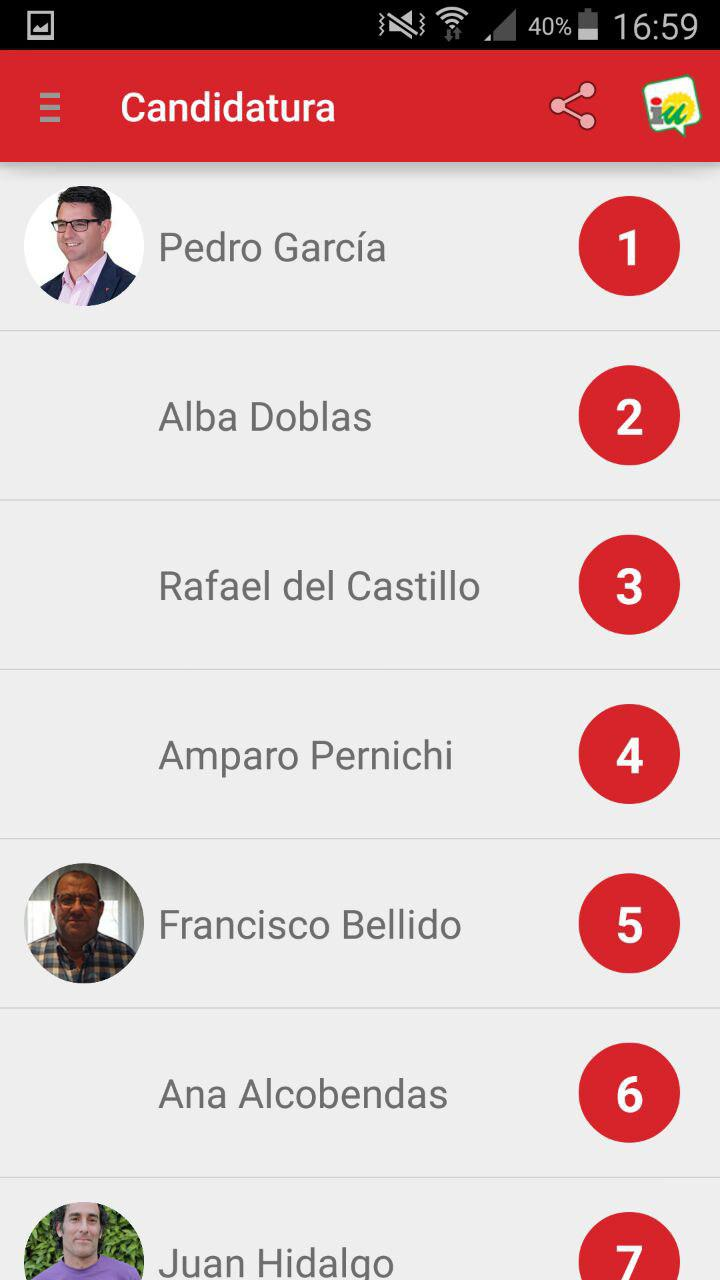
\includegraphics[width=\textwidth]{Media/Captures/IURecuperaCordobaCandidates.jpg}
                \caption{Candidatos}
                \label{fig:iuCandidates}
        \end{subfigure}
        \caption{Capturas de $\sharp$IURecuperaCórdoba}
        \label{fig:iuRecuperaCordoba}
\end{figure}

 - \underline{Aspectos positivos}:

\begin{itemize}
	\item Interfaz limpia y sencilla de diseño plano.
	\item Consistencia en la aplicación: la información se presenta siempre en formato de lista ofreciendo los minimos datos necesarios sin sobrecargar de información al usuario.
	\item Menú lateral disponible en cualquier pantalla con las principales acciones de la aplicación: Candidatos, Programa, Videos y Noticias.
	\item El programa electoral está estructurado en un indice primer nivel y a veces con segundo nivel.
	\item Aporta la opción de ver el programa completo. 
\end{itemize}

 - \underline{Aspectos negativos}:

\begin{itemize}
	\item Utiliza a veces iconos cuyo proposito no se entiende: ¿Un avión de papel para noticias? ¿Un ''a$>$z'' para la lista de candidatos?
	\item Las distintas secciones se abren dentro de la aplicación, pero da acceso a una navegación lateral por las páginas del PDF del programa en cuestión.
	\item Si haces zoom en una sección no permite pasar de página.
\end{itemize}

\subsubsection{PSOE Andalucía}

Esta app presenta la candidatura del PSOE a la junta de Andalucía para las elecciones del 22 de Marzo, promocionando básicamente su programa electoral y a la candidata Susana Díaz. Permite también estar al día de noticias y eventos relacionados con dicha candidatura.

La navegación por el programa, aunque estructurada en un primer nivel, se realiza directamente visualizando páginas que parecen extraidas del programa en PDF.

\begin{figure}[H]
        \centering
        \begin{subfigure}[b]{0.3\textwidth}
                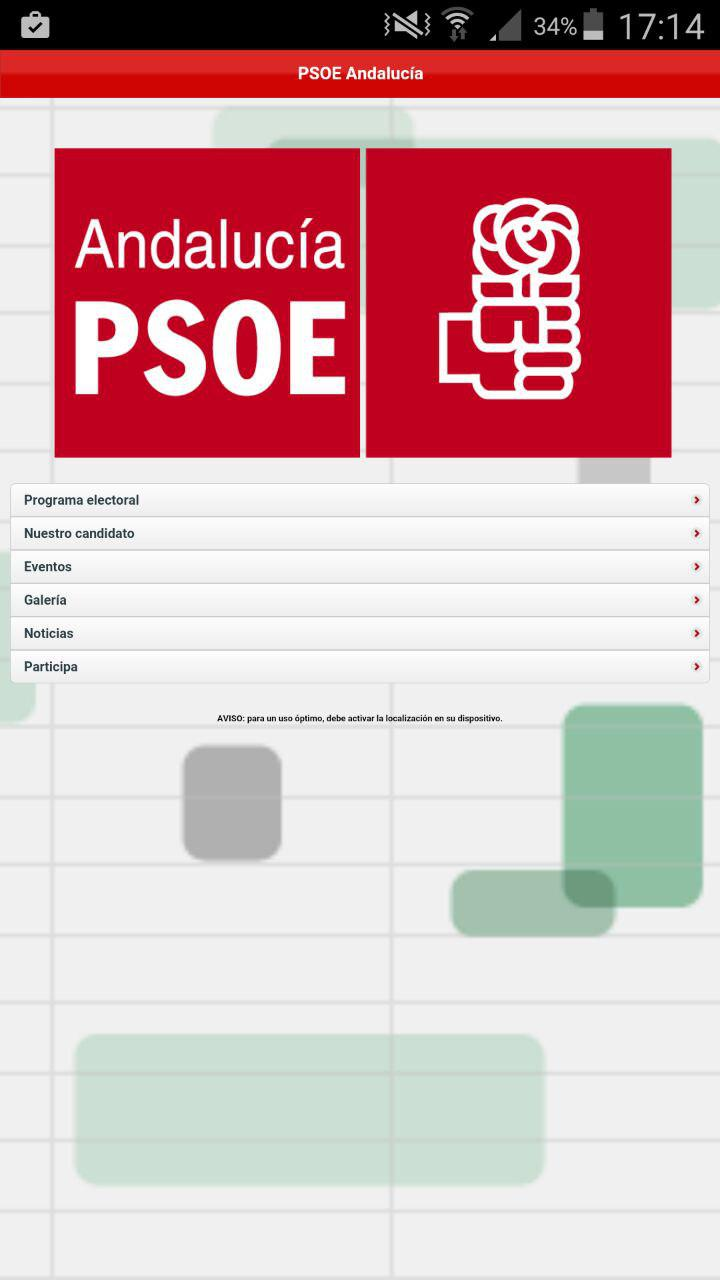
\includegraphics[width=\textwidth]{Media/Captures/psoeAndalucia.jpg}
                \caption{Pantalla Principal}
                \label{fig:psoePpal}
        \end{subfigure}
        ~
        \begin{subfigure}[b]{0.3\textwidth}
                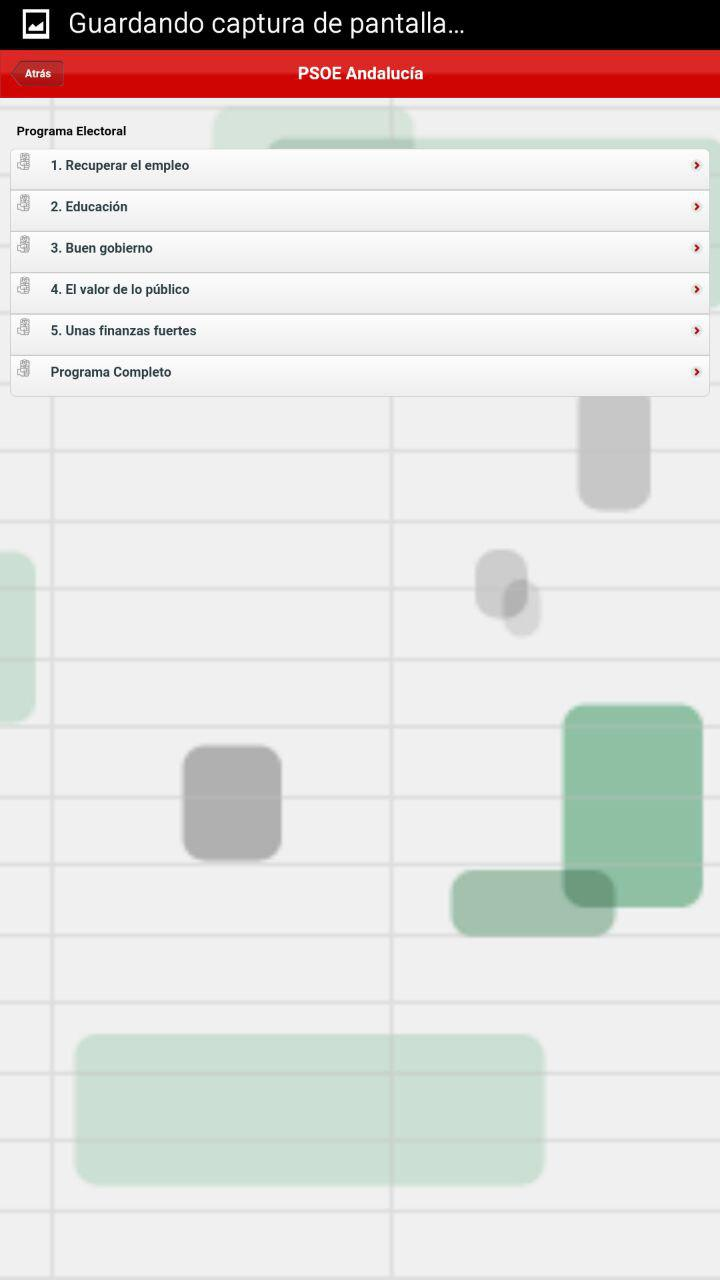
\includegraphics[width=\textwidth]{Media/Captures/psoeAndaluciaIndex.jpg}
                \caption{Indice Programa}
                \label{fig:psoeIndex}
        \end{subfigure}
        ~
        \begin{subfigure}[b]{0.3\textwidth}
                
\includegraphics[width=\textwidth]{Media/Captures/psoeAndaluciaSection.jpg}
                \caption{Sección Programa}
                \label{fig:psoeSection}
        \end{subfigure}
        \caption{Capturas de PSOE Andalucia}
        \label{fig:psoeAndalucia}
\end{figure}

 - \underline{Aspectos positivos}:

\begin{itemize}
	\item Posee un indice de primer nivel para estructurar el programa.
\end{itemize}

 - \underline{Aspectos negativos}:

\begin{itemize}
	\item La interfaz y los botones no se adaptan al tamaño de pantalla y permanecen de un tamaño pequeño que dificulta la interacción.
	\item El programa electoral se visiona en forma de una página que parece descargada directamente de la version PDF y que permanece en un tamaño pequeño e ilegible, no permitendo tampoco hacer zoom.
	\ En general, la interfaz parece hecha para una web más que para un móvil. 
\end{itemize}

\subsubsection{PP Canarias}

La delegación del Partido Popular en Canarias presenta su aplicación móvil para promocionar a sus candidatos para las elecciones autonómicas y municipales de Mayo de 2015. La aplicación nos avisará de los eventos electorales, podremos consultar los candidatos, novedades, galería de imágenes y por supuesto ver el programa electoral.

\begin{figure}[H]
        \centering
        \begin{subfigure}[b]{0.3\textwidth}
                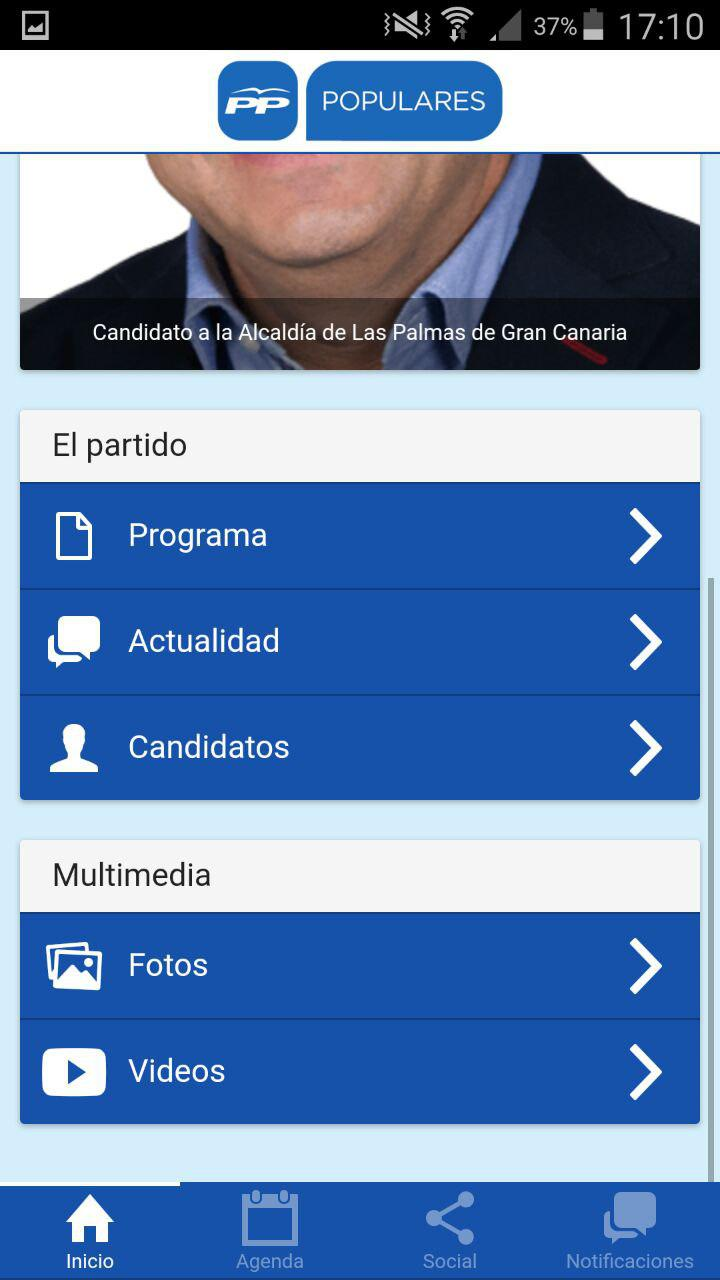
\includegraphics[width=\textwidth]{Media/Captures/ppCanarias.jpg}
                \caption{Pantalla Principal}
                \label{fig:ppIndex}
        \end{subfigure}
        ~
        \begin{subfigure}[b]{0.3\textwidth}
                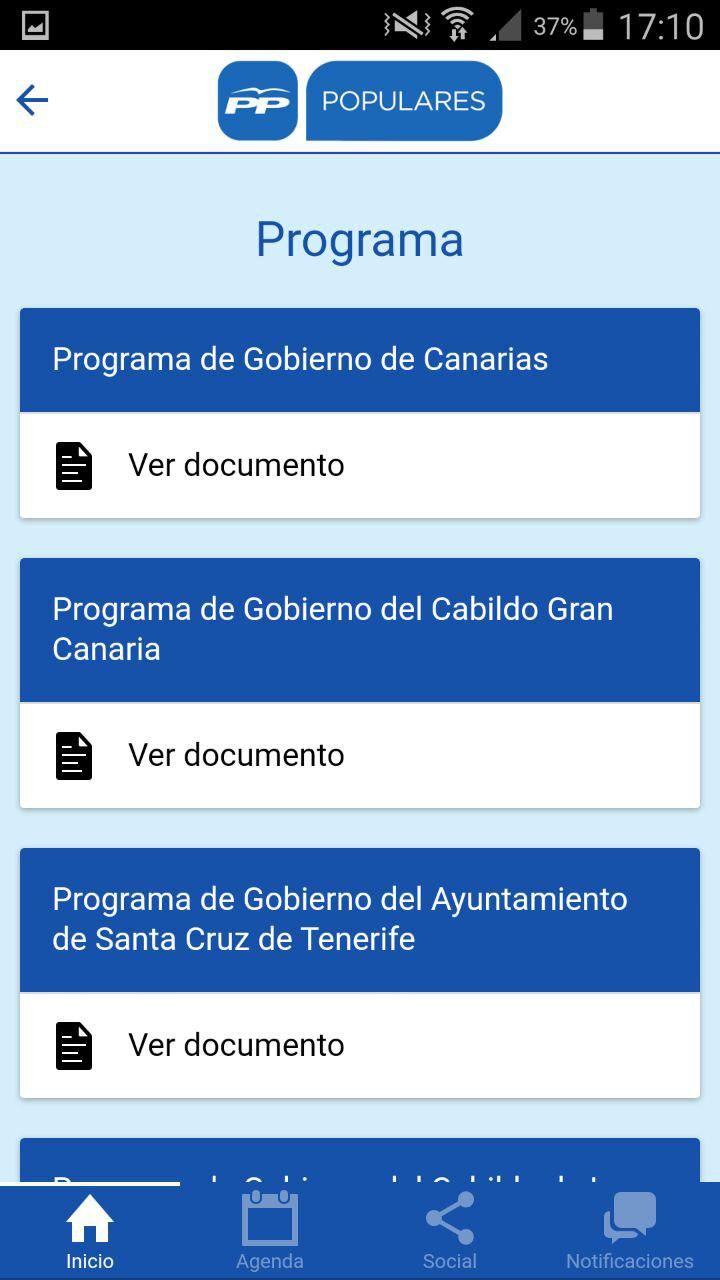
\includegraphics[width=\textwidth]{Media/Captures/ppCanariasProgram.jpg}
                \caption{Programas}
                \label{fig:ppPrograms}
        \end{subfigure}
        ~
        \begin{subfigure}[b]{0.3\textwidth}
                
\includegraphics[width=\textwidth]{Media/Captures/ppCanariasCandidates.jpg}
                \caption{Candidatos}
                \label{fig:ppCandidates}
        \end{subfigure}
        \caption{Capturas de PP Canarias}
        \label{fig:ppCanarias}
\end{figure}

 - \underline{Aspectos positivos}:

\begin{itemize}
	\item Interfaz limpia y atractiva con una organización clara en secciones que aparecen en una barra inferior al estilo de iOS.
\end{itemize}

 - \underline{Aspectos negativos}:

\begin{itemize}
	\item Aunque dispone de una sección para programas electorales, no dispone de ellos en local, si no que te obliga a abrir un navegador para ver la versión entera en PDF.
	\item El problema de la barra inferior de menús es que quita espacio al contenido principal. Se podría haber puesto el menú en alun sitio menos intrusivo.
\end{itemize}

\subsection{Participación Ciudadana} \label{ssec:artProposals}

Centrándonos en la participación ciudadana ya sea mediante la generación de Propuestas, el desarrollo colaborativo de programas o la recogida de firmas, existen numerosos portales en Internet y aplicaciones móviles destinadas a ello. Realizaremos un breve repaso a las aplicaciones más destacadas.

\subsubsection{Reddit}

Reddit \cite{ref:reddit} es una plataforma web de código libre donde los usuarios pueden crear temas, propuestas o compartir enlaces web a otros sitios. A primera vista puede parecer un foro, aunque la principal diferencia respecto a éste último radica en que otros usuarios pueden votar a favor o en contra de los enlaces, haciendo que el sistema los haga aparecer como más o menos destacados. A esto lo denominan ''filtrado colaborativo'' pues de esta forma los temas de conversación, enlaces, o propuestas aparecerán en el orden que haya escogido la comunidad según la puntuación positiva o negativa que le hayan dado. 
En principio el uso de reddit está destinado a todo tipo de temas, entre los que podemos encontrar algunos ejemplos fuertemente relacionados con la participación ciudadana. Es el caso de Plaza Podemos \cite{ref:plazaPodemos}: un espacio utilizado para que la ciudadanía pueda expresar sus propuestas, compartir noticias relacionadas con la actualidad política o debatir aquellos temas que más les preocupan. Así, aunque no seamos participantes de reddit, de un simple vistazo podemos saber qué es lo más debatido por la ciudadanía, las propuestas que quieren llevar a cabo en en el gobierno o cuáles son los temas que más les preocupan.

\begin{figure}[H]
\centering
\includegraphics[keepaspectratio, scale=0.30]{Media/Captures/plazaPodemos.png}
\caption{Plaza Podemos utilizando la plataforma Reddit}
\label{fig:plazaPodemos}
\end{figure}

 - \underline{Aspectos positivos}:

\begin{itemize}
	\item Opción de filtrado por tipos de contenido (propuestas, noticias...) y ordenación de distintas formas (nuevos, populares, activos...)
	\item Sistema de votación sencillo desde la propia previsualización del contenido mediante flechas (arriba y abajo), pudiendo ver entre ellas el número actual de votos.
\end{itemize}

 - \underline{Aspectos negativos}:

\begin{itemize}
	\item Para un usuario que lo usa por primera vez puede resultar confuso que haya contenido redactado con usuarios mezclado con enlaces a noticias externas.
\end{itemize}

\subsubsection{Change.org}

Change.org \cite{ref:changeOrg} es un portal web que permite lanzar múltiples peticiones de cambio en Internet. Podríamos definirlo como la evolución de la recogida de firmas en la calle: cualquiera puede realizar una petición para solicitar el apoyo de otros. Las personas que decidan apoyar la petición, dejarán sus datos personales y constarán entre el número de personas que han firmado a favor de la petición. Una vez que han alcanzado un número objetivo de apoyos se procede a entregar las firmas digitales al organismo, persona o entidad a la que va destinada la petición.

Por ejemplo: en mayo de 2011, en relación con las movilizaciones del Movimiento 15-M y Democracia Real Ya, y ante el desalojo por los Mossos de Esquadra se llevó a cabo la petición “Exige la dimisión fulminante del Conseller de Interior Felip Puig por la violencia utilizada en Pza. Catalunya”.

Desde su creación en 2007, Change.org ha logrado muchas de sus peticiones demandadas entre los que se incluyen la atención de pacientes con enfermedades complejas, protección sobre animales y medio ambiente, derechos públicos, leyes, etc.

\begin{figure}[!]
\centering

\includegraphics[keepaspectratio, scale=0.30]{Media/Captures/changeOrg.png}
\caption{Change.org · La mayor plataforma de peticiones del mundo}
\label{fig:changeOrg}
\end{figure}

 - \underline{Aspectos positivos}:

\begin{itemize}
	\item Página principal con peticiones cuyo objetivo de firmas se ha conseguido (''victoria'') y las más destacadas aun por conseguir.
	\item De cada petición se muestra un ''preview'' con los aspectos más destacados: foto, titulo, autor, número de firmas y fecha de creación.
\end{itemize}

 - \underline{Aspectos negativos}:

\begin{itemize}
	\item Aunque existen filtros para peticiones (Destacadas, Populares y Recientes) ¿de qué depende esta clasificación? No queda claro cómo se elige la opción en dicha lista de peticiones,
\end{itemize}

\subsubsection{Programas Colaborativos de Ahora Madrid y Zaragoza en Común}

Para las pasadas elecciones municipales del 24 de Mayo, la candidatura de unidad popular Ahora Madrid, desarrolló una plataforma en la web para elaborar su programa electoral de forma colaborativa. En esta plataforma, cualquier usuario tenía la oportunidad de explorar las propuestas por categoría o por distrito. De tal forma que podría debatirlas, puntuarlas o crear sus propias propuestas. Así las propuestas más valoradas por la comunidad, serían llevadas al programa final para las elecciones municipales del 24 de Mayo.

El resultado final fue determinar las cinco propuestas más votadas que fueron incluidas en el programa final como medidas urgentes para realizar en los 100 primeros días de gobierno. 

\begin{figure}[!]
\centering

\includegraphics[keepaspectratio, scale=0.25]{Media/Captures/programaAhoraMadrid.jpg}
\caption{Creación colaborativa del programa de Ahora Madrid.}
\label{fig:programaAhoraMadrid}
\end{figure}

También utilizaron una plataforma similar en la candidatura zaragozana de unidad popular Zaragoza en Común \cite{ref:ganemosZaragoza}.

\begin{figure}[!]
\centering

\includegraphics[keepaspectratio, scale=0.30]{Media/Captures/programaColaborativoGanemosZaragoza.png}
\caption{Creación colaborativa del programa de Zaragoza en Común.}
\label{fig:programaZaragozaEnComun}
\end{figure}

 - \underline{Aspectos positivos}:

\begin{itemize}
	\item Las propuestas están organizadas por distintos temas: ''Ejes temáticos'' en el caso de Zaragoza en Común y ''Areas y Objetivos'' en el caso de Ahora Madrid.
	\item En ambos casos se puede filtrar la lista de propuestas de distintas formas (''Más valoradas'', ''Más consenso'' y ''Más debatidas'') 
	\item En el ''preview'' de la propuesta se muestra el número de comentarios y el porcentaje de votos positivos en relación al número total de votos recibidos.
\end{itemize}

 - \underline{Aspectos negativos}:

\begin{itemize}
	\item En cada propuesta se muestra un número a la izquierda que no explica lo que significa (entendemos que es el número de votos a favor).
\end{itemize}

\subsubsection{Appgree}

Appgree\cite{ref:appgree} es una plataforma desarrollada con el objetivo de poner a grandes grupos de personas de acuerdo en poco tiempo. Está disponible tanto para web como para móviles y permite que sus usuarios lancen propuestas y debatan sobre cualquier tema pudiendo votar y alcanzar un consenso, obteniendo los resultados de dicha votación casi en tiempo real gracias a un algoritmo estadístico desarrollado por ellos llamado DemoRank\cite{ref:appgree_demoRank}.

En la aplicación podemos acceder a una lista de canales: que aglutinan encuestas, propuestas y preguntas (ya sea de respuesta abierta o de votación entre dos o mas opciones), pudiendo votar y ver los resultados actuales de votación y respuestas. Para fomentar la participación potencian mucho el uso de listas de preguntas más candentes y recientes. Además se pueden compartir preguntas por redes sociales para aumentar su difusión.

\begin{figure}[H]
        \centering
        \begin{subfigure}[b]{0.3\textwidth}
                
\includegraphics[width=\textwidth]{Media/Captures/appgreeChannel.jpg}
                \caption{Canal}
                \label{fig:appgreeChannel}
        \end{subfigure}
        ~
        \begin{subfigure}[b]{0.3\textwidth}
                
\includegraphics[width=\textwidth]{Media/Captures/appgreeQuestion.jpg}
                \caption{Pregunta Múltiple}
                \label{fig:appgreeQuestion}
        \end{subfigure}
        ~
        \begin{subfigure}[b]{0.3\textwidth}
                
\includegraphics[width=\textwidth]{Media/Captures/appgreeOpenQuestion.jpg}
                \caption{Pregunta Abierta}
                \label{fig:appgreeOpenQuestion}
        \end{subfigure}
        \caption{Capturas de Appgree}\label{fig:appgreeCaptures}
\end{figure}

 - \underline{Aspectos positivos}:

\begin{itemize}
	\item Interfaz limpia de colores planos (blanco y azul) con pantalla principal de ultimas preguntas destacadas.
	\item Organización por canales temáticos de las preguntas.
	\item Opción de marcar canales como favoritos para poder seguirlos y ser notificados de las últimas preguntas añadidas.
\end{itemize}

 - \underline{Aspectos negativos}:

\begin{itemize}
	\item Las preguntas se organizan por antigüedad (activas y no activas) pero se navega de abajo hacia arriba, cuando uno esperaria hacerlo al revés.
	\item Los tipos de preguntas (abiertas, de respuesta múltiple, de sí o no, encuestas...) aparecen todas mezcladas.
\end{itemize}

\newpage
\thispagestyle{sectioned}
\chapter{Tecnologías del Proyecto}

En las siguientes secciones explicaremos brevemente las tecnologías y herramientas que hemos utilizado para llevar a cabo este proyecto. Concretamente hablaremos de las tecnologías utilizadas durante la Migración del cliente web de SwellRT (Wave) a Android y durante el desarrollo de la aplicación Android que hará uso del resultado de dicha Migración. 

En el caso de Wave, al tratarse de una tecnología bastante reciente, se explicacrá más detalladamente en qué consite esta tecnología, pero para el resto de casos se hará una pequeña reseña sobre en qué consiste la tecnología y sus usos. En todos los casos se intentará tambíen explicar de qué manera y para qué se ha utilizado dentro de este proyecto.

Para hacerse una idea general de las tecnologías utilizadas se recomienda ver el resumen que se muestra en la Tabla \ref{fig:technologiesTable}. 
 
      \begin{table}[H]
	\footnotesize
	\begin{center}
	\begin{tabular}{| c | c | m{9cm} | c |}
	  \hline
	  \textbf{Tipo} & \textbf{Nombre} & \textbf{Uso} & \textbf{Sección} \\
	  \hline
	  \multirow{2}{*}{API} & SwellRT & Base de la que se parte para la Migración de Wave a Android & \ref{sssec:swellRT} \\ \cline{2-4} 
	  & Android & Plataforma para la Migración y el Desarrollo de la app. & \ref{ssec:android} \\ \hline
	  \multirow{2}{*}{Servidor} & \begin{tabular}[c]{@{}c@{}}Wave In A Box\\ (WIAB)\end{tabular} & Servidor que aloja las Waves. Migración y Desarrollo de la App. & \ref{sssec:wiab} \\ \cline{2-4} 
	  & OpenShift & Servidor que aloja el Service REST y la Base de Datos de la App. & \ref{ssec:openshift} \\ \hline
	  \multirow{5}{*}{Lenguaje} & Java & Lenguaje base para trabajar con Android, tanto en la Migración como en la App. & \ref{ssec:java} \\ \cline{2-4} 
	  & JavaScript & Lenguaje del antiguo cliente web de Wave presente en SwellRT. & \ref{ssec:javascript} \\ \cline{2-4} 
	  & PHP & Lenguaje para definición del Service REST de la App. & \ref{ssec:php} \\ \cline{2-4} 
	  & SQL & Lenguaje para definir e interactuar con la Base de Datos de la App. & \ref{ssec:sql} \\ \cline{2-4} 
	  & XML & Lenguaje para definición de interfaces en Android. & \ref{ssec:xml} \\ \hline
	  \begin{tabular}[c]{@{}c@{}}Formato\\  de Datos\end{tabular} & JSON & Formato para intercambio de información con Servidor Wave y REST. & \ref{ssec:json} \\ \hline
	  \multirow{2}{*}{Framework} & GWT & \begin{tabular}[c]{@{}c@{}}Framework JavaScript utilizado por el antiguo Cliente web \\ de Wave presente en SwellRT.\end{tabular} & \ref{ssec:gwt} \\ \cline{2-4} 
	  & Laravel 5 & Framework de desarrollo del Service REST de la App en PHP. & \ref{ssec:laravel} \\ \hline
	  \multirow{3}{*}{Protocolo} & Google Wave & Protocolo de intercambio de Waves usado para la migración y la App. & \ref{ssec:wave} \\ \cline{2-4} 
	  & HTTP & \begin{tabular}[c]{@{}c@{}}Protocolo de transferencia de datos por Internet \\ usado por la Migración y por la app.\end{tabular} & \ref{ssec:http} \\ \cline{2-4} 
	  & WebSocket & \begin{tabular}[c]{@{}c@{}}Protocolo de transferencia de datos bidireccionales por \\ Internet, usado por la Migración y por la App.\end{tabular} & \ref{ssec:websocket} \\ \hline
	  \multirow{2}{*}{\begin{tabular}[c]{@{}c@{}}Base de \\ Datos\end{tabular}} & MySQL & Sistema Gestor de la Base de Datos de la App & \ref{ssec:mysql} \\ \cline{2-4} 
	  & PhpMyAdmin & Herramienta de Administración de la Base de Datos de la App. & \ref{ssec:phpmyadmin} \\ \hline
	  \multirow{2}{*}{\begin{tabular}[c]{@{}c@{}}Control de\\ Versiones\end{tabular}} & Git & Software de control de versiones usado para la Migración y la App. & \ref{ssec:git} \\ \cline{2-4} 
	  & GitHub & \begin{tabular}[c]{@{}c@{}}Plataforma web de control de versiones que aloja\\ los desarrollos de la Migración y de la App.\end{tabular} & \ref{ssec:github} \\ \hline
	  Prototipado & POP & \begin{tabular}[c]{@{}c@{}}Aplicación para elaborar los Prototipos Interactivos \\ basados en los Prototipos en Papel de la App.\end{tabular} & \ref{ssec:pop} \\ \hline
	  \multirow{3}{*}{IDE} & Eclipse Luna & Entorno de Desarrollo utilizado para la Migración de Wave. & \ref{ssec:eclipse} \\ \cline{2-4} 
	  & Android Studio & Entorno de Desarrollo utilizado para el desarrollo de la App. & \ref{ssec:androidStudio} \\ \cline{2-4} 
	  & Sublime Text & \begin{tabular}[c]{@{}c@{}}Editor de texto y de código fuente,utilizado para\\ desarrollar el Service REST.\end{tabular} & \ref{ssec:sublime} \\ \hline
	\end{tabular}
	\end{center}
	\caption{Tecnologías usadas en el Proyecto}
	\label{fig:technologiesTable}
      \end{table}
    
\section{Tecnologías de Wave}
  
  \subsection{Google Wave}\label{ssec:wave}

  Ideado y presentado en 2009 por ingenieros de Google \cite{ref:wave_announcement}, Wave es a la vez un protocolo de comunicaciones \cite{ref:wave_over_xmpp} y una plataforma web de código libre, que permiten a sus usuarios comunicarse y colaborar entre sí en tiempo real (Ver sección \ref{sssec:realTime}) y de forma federada (Ver sección \ref{sssec:federation}) a través de Internet. 
  Inicialmente fue desarrollado con el objetivo de integrar en una sola plataforma servicios ampliamente utilizados como son el correo electrónico, las redes sociales y la mensajería instantánea. Pese al gran entusiasmo generado entre la comunidad de desarrolladores tras su anuncio, en el año 2010 Google anuncia el abandono del proyecto \cite{ref:google_wave_end} debido a su poca acogida entre los desarrolladores y a que decide reorientar el uso de la tecnología hacia sus plataformas de edición de documentos Google Docs \cite{ref:google_docs} y a su red social Google + \cite{ref:google_plus}.  Es en este momento cuando el desarrollo libre del proyecto pasa a manos de la Apache Software Foundation bajo el nombre de Apache Wave.

  \subsection{Apache Wave}
  
  Al cambiar de manos su desarrollo en 2010, la tecnología pasa a formar parte de la incubadora de la fundación Apache \cite{ref:apache_wave_about} como software de código libre bajo licencia Apache \cite{ref:apache_license}. Así, se produce el desarrollo de Wave In a Box (WIAB) (Ver sección \ref{sec:wiab}), plataforma que integra un cliente web sencillo y una implementación de un servidor Wave que cualquiera puede descargar y desplegar en su ordenador.
  
  \subsection{Características de Wave}
  
  Como plataforma de código libre desarrollada para ser utilizada en red, Wave hace uso de distintas tecnologías y protocolos bien conocidos. Entre sus características más destacadas están las siguientes:

    \subsubsection{Federación}\label{sssec:federation}
    
    El Protocolo Wave \cite{ref:wave_over_xmpp} fue desarrollado para utilizar un modelo federado \cite{ref:wave_federation} \cite{ref:wave_white_paper} de comunicación basado en la tecnología XMPP \cite{ref:xmpp} \cite{ref:wave_over_xmpp}. Se trata por tanto de un modelo descentralizado en el que cualquiera de los participantes en la conversación es libre de actuar tanto como servidor como cliente sin que ello afecte a su participación en la conversación. 
    Además, a diferencia de otras tecnologías (como el correo electronico) en las que cada participante almacena su propia copia de la conversación y cada vez que hay cambios se debe transmitir la conversación entera a todos los participantes, Wave tiene la ventaja de que actúa de forma que es el servidor de la conversación el único que almacena la copia entera y se encarga de calcular los cambios que se han producido para transmitir solamente dichos cambios por la red a los participantes, con las consiguientes ventajas en términos de latencia que ello conlleva. 

    \subsubsection{Consistencia en tiempo real}\label{sssec:realTime}
    
    El Protocolo Wave \cite{ref:wave_over_xmpp} utiliza la tecnología de Transformaciones Operacionales (OT) \cite{ref:how_ot_works} para garantizar la consistencia en la comunicación en tiempo real entre los participantes. Es decir, cualquier cambio producido por cualquiera de los participantes en la conversación se transmite automáticamente y en tiempo real al resto de los participantes sin pérdida de información y garantizando que los cambios se muestran en el estricto orden en el que se produjeron sin errores \cite{ref:wave_ot}.
    
    \subsubsection{Escalabilidad}
    
    Wave fue desarrollado como un protocolo de alta escalabilidad que permite gestionar la existencia de una gran cantidad de conversaciones y participantes sin que por ello se resienta la productividad del sistema.
    
    \subsection{Servidores Wave}
  
    \subsubsection{Wave in a Box}\label{sssec:wiab}
    
    Wave In a Box (WIAB) \cite{ref:wave_in_a_box} es el nombre de la implementación de un servidor Wave desarrollado por la Apache Software Foundation tras pasar el proyecto a sus manos en el año 2012. Al igual que el resto del código de la tecnología que heredó de Google, está implementado en Java usando OpenJDK \cite{ref:openjdk}. La instalación trae consigo un cliente web desarrollado en Javascript usando el framework Google Web Toolkit (GWT) \cite{ref:gwt}. Este cliente web sirve como prueba de concepto de las funcionalidades básicas del Modelo Conversacional de Wave, pudiendo gesionar waves, usuarios y extensiones. Actualmente cualquiera puede descargar y desplegar WIAB en su ordenador siguiendo los pasos que nos proporcionan en su wiki \cite{ref:wave_in_a_box_wiki}. La aplicación se distribuye en forma de código fuente, accesible entre otras formas desde su repositorio de GitHub \cite{ref:wave_in_a_box_github}. Existen asimismo servidores de prueba ya desplegados en Internet sobre los que se puede observar el funcionamiento de WIAB \cite{ref:wave_in_a_box_server}.
   
   
    \subsubsection{SwellRT}\label{sssec:swellRT}
    
    Como parte del proyecto europeo P2PValue \cite{ref:p2pvalue} existe SwellRT (Swell Real Time), un fork de WIAB que amplía las características de éste último añadiendo un nuevo modelo de datos (Modelo de Datos Colaborativo) más allá del Modelo de Datos Conversacional de Wave original. Proporciona también un API escrito en Java que permite trabajar sobre los datos de ese nuevo modelo en forma de tres tipos básicos: mapas, listas y strings. Es por tanto un framework de colaboración en tiempo real que basa su funcionamiento en Apache Wave y cuyo principal popósito es permitir la integracion de la tecnología Wave en otras aplicaciones, que podrán compartir objetos (de los tipos antes mencionados) de forma federada y en tiempo real. Su código fuente está disponible en GitHub \cite{ref:swellRT_github}, así como sus instrucciones de instalación (Ver el Readme en GitHub).\\[.2cm]

    Para este proyecto se ha usado el framework SwellRT como base para la migración de la tecnología de Apache Wave a la plataforma Android \cite{ref:android_platform}. Se pretende con esto que SwellRT haga uso de las funcionalidades nativas de Android.
    
    \subsection{Eclipse}\label{ssec:eclipse} 
    
	Eclipse \cite{ref:eclipse} es un Entorno de Desarrollo Integrado (IDE) open-source (bajo licencia Eclipse Public License) desarrollado por la Eclipse Foundation. Lanzado en 2007 alcanza actualmente su versión 4.4, también denominada Eclipse ''Luna''. Se trata de uno de los IDEs más utilizados que proporciona herramintas que permiten el desarrollo de código para múltiples lenguajes y tecnologías. Posee además la capacidad de extender sus capacidades gracias al uso de plug-ins que se pueden descargar desde su marketplace. Es el caso por ejemplo del plugin ADT (Android Developer Tools), que permite utilizar el SDK de Android para desarrollar para esta plataforma utilizando Eclipse como IDE. Hasta finales del año 2014 Eclipse + ADT era el IDE recomendado por Google para el desarrollo en su plataforma móvil, aunque recientemente ha pasado a utilizar su propio IDE llamado Android Studio (Ver Sección \ref{ssec:androidStudio})
	
	En este proyecto usaremos Eclipse con el plugin ADT como IDE para estudiar el código del cliente web de SwellRT y llevar a cabo una migración a Android que permita hacer uso de las características nativas de esta plataforma.
    
    \subsection{Java}\label{ssec:java}
    
	Java \cite{ref:java} es un lenguaje de programación de próposito general y orientado objetos. Fue desarrollado en 1995 por Sun Microsystems, actualmente parte de Oracle, y se distribuye en forma de JDK (Java Development Kit), cuya versión oficial privativa alcanza hoy en día la 8. Existe no obstante una versión de código libre (bajo licencia GPLv2) llamada Open JDK \cite{ref:openjdk} disponible actualmente en su versión 7. Java tiene como ventaja su independencia del hardware, ya que cualquier código compilado en java se traduce a un formato bytecode que se ejecuta en una Máquina Virtual Java (JVM) que es independiente del hardware que haya por debajo.
	
	En este proyecto usaremos Java para la Migración del cliente SwellRT a Android, pues dicho cliente (y el que desarrollo Google inicialmente) esta escrito en su mayor parte en este lenguaje de programación. Lo utilizaremos también para el desarrollo de la app, ya que el SDK de Android se basa en Java para desarrollar código para dicha plataforma.
    
    \subsection{GWT}\label{ssec:gwt}
    
	GWT \cite{ref:gwt} (Google Web Toolkit) es un framework de código libre (bajo licencia Apache 2.0) que facilita el desarrollo de aplicaciones web basadas en AJAX y JavaScript. Concretamente el API de GWT permite desarollar cñódigo en Java que posteriormente será traducido a JavaScript. Fue creado por Google en 2006 y actualmente es un proyecto independiente open-source que alcanza ya su versión 2.7
	
	En este proyecto utilizaremos GWT durante la Migración de Wave a Android. ya que una parte significativa del cliente web de SwellRT está desarrollada con esta tecnología y es necesario estudiar el código para sustituirla por código nativo de Android, ya que la plataforma móvil de Google no es compatible con GWT.
    
    \subsection{JavaScript}\label{ssec:javascript}
    
	JavaScript \cite{ref:javascript} (JS) es un lenguaje de programación dinámico y débilmente tipado utilizado a menudo para la programación de aplicaciones web del lado del cliente (navegador web), aunque también existen implementaciones para el lado del servidor (como Node.js). Originalmente desarrollado en 1995 por la extinta Netscape Communications, su versión actual es la 1.8.5.  
	
	En este proyecto se utilizará JavaScript para estudiar la implementación del cliente web de SwellRT hecha con GWT y JavaScript que deberemos migrar a código nativo de Android, pues la plataforma móvil de Google no es compatible de forma nativa con JavaScript.
    
    \subsection{HTTP}\label{ssec:http}
    
	HTTP \cite{ref:http} (HyperText Transfer Protocol) es el protocolo de capa de aplicación más utilizado para establecer comunicaciones en la World Wide Web. Fue desarrollado en 1996 conjuntamente por la World Wide Web Consortium (W3C) y el Internet Engineering Taskforce (IETF), aunque la definición de su versión más actual (1.1) se encuentra especificada en la serie de RFCs (Request For Comments) 7230 \cite{ref:http}. Se trata de un protocolo orientado a transacciones que siguen un esquema de petición-respuesta entre cliente y servidor. 
	
	En este proyecto utilizaremos el protocolo HTTP para establecer las conexiones con ambos servidores: el servidor SwellRT que aloja las Waves y el servidor Openshift que aloja el Service REST y la Base de Datos de la aplicación. Concretamente con este protocolo realizaremos el proceso de login en Wave y las peticiones al Service REST en la aplicación Android.
    
    \subsection{WebSocket}\label{ssec:websocket}
    
	WebSocket \cite{ref:webSocket_ref} es un protocolo que permite establecer comunicaciones bidireccionales (de cliente a servidor y viceversa) y full-dúplex (de forma simúltánea en ambos sentidos) en la red. Permite utilizar la tecnología de los sockets TCP en la capa de aplicación.  Se trata de un protocolo estandarizado por la IETF en 2011 en el RFC 6455 \cite{ref:webSocket_ref}. 
	
	En este proyecto utilizaremos esta tecnología para establecer un canal de comunicación basado en sockets con el servidor Wave de SwellRT, pues la característica de bidireccionalidad full-dúplex es necesaria para aprovechar la potencialidad de consistencia en tiempo real de Wave. Concretamente en la Migración deberemos sustituir la implementación actual de WebSocket en GWT por otra que sea compatible de forma nativa con Android.
    
    \subsection{Git}\label{ssec:git} 
    
	Git \cite{ref:git} es un Sistema de Control de Versiones (VCS) distribuido y open-source (bajo licencia pública GNU) diseñado para gestionar las distintas versiones de una aplicación independientemente del tamaño de la aplicación y del número de personas que trabajan en ella. Fue creado por Linus Torvalds en 2005 para trabajar en el desarrollo del kernel de Linux, aunque  su versión actual (2.4.2) es una de las herramientas  de control de versiones mas utilizada para gestionar proyectos software. Su interfaz es por consola de comandos.
	
	En este proyecto usaremos Git por consola de comandos como Sistema de Control de Versiones de todo el software generado, tanto de la Migración de Wave/SwellRT a Android como del desarrollo de la app y el Service REST del que hace uso. Incluso las distintas versiones del código látex de esta Memoria estará gestionado con Git.
     
    \subsection{GitHub}\label{ssec:github}
    
    GitHub \cite{ref:github} es una plataforma web lanzada en 2008 que permite alojar de forma gratuita y en sitios llamados repositorios, proyectos software que utilicen Git como Sistema de Control de Versiones. Los repositorios gratutos son públicos y accesibles por todo el mundo, de manera que cualquiera puede participar en la elaboración de código, aunque existe la opción de pagar por tener acceso a repositorios privados. GitHub proporciona una interfaz web que además de gestionar los repositorios permite alojar wikis, páginas web, gestión de tareas pendientes (issues) y control de acceso entre otras funcionalidades.
    
    Para este proyecto utilizaremos GitHub como plataforma para alojar todo el código open-source desarrollado durante el proyecto: la Migración de SwellRT a Android (cuyo cliente web antiguo también está disponible en GitHub \cite{ref:swellRT_github}), el desarrollo de la aplicación Android, el Service REST y la Memoria. Todo esto esta disponible en forma de repositorios bajo la organización llamada ''Zorbel'' en la siguiente URL:
    
    \url{https://github.com/Zorbel}    

\section{Tecnologías de la Aplicación Android}
    
    \subsection{Android Studio}\label{ssec:androidStudio}
    
	Android Studio \cite{ref:android_studio} es el Entorno de Desarrollo Integrado (IDE), basado en IntelliJ IDEA \cite{ref:intelliJ_Idea}, oficial que Google proporciona para desarrollar aplicaciones para Android. Fue anunciado en 2013 y en diciembre de 2014 dejó su fase de beta y pasó a ser el IDE de referencia para el desarrollo en Android, dejando atrás el antiguo IDE de Eclipse junto al plug-in ADT. Android Studio integra en un solo lugar todas las herramientas necesarias para desarrollar en esta plataforma como un gestor de versiones de Android (SDK Manager), un gestor de emuladores virtuales (AVD Manager) o una herramienta de Debug (DDMS) entre otras. Permite asimismo trabajar tanto con código de aplicación como con la interfaz gráfica (XML), la cual podremos previsualizar en el propio IDE.
	
	En este proyecto, y ya que desde principio de año es el IDE de referencia, utilizaremos Android Studio para el desarrollo de la aplicación Android que hará uso de las funcionalidades de Wave.
    
    \subsection{Android}\label{ssec:android}
    
	Android \cite{ref:android_platform} es el Sistema Operativo de código libre (bajo licencia Apache 2.0) para dispositivos móviles de Google basado en el kernel de Linux. Lanzado en 2007, actualmente su API alcanza ya la versión 21 \cite{ref:android_api21}, también denominada Android 5.0 ''Lollipop''. Para desarrollar en esta plataforma basta con descargarse su SDK \cite{ref:android_sdk}, accesible entonces desde desde consola de comandos, aunque siempre resulta más cómodo utilizar un Entorno de Desarrollo como Eclipse o Android Studio (Ver Secciones \ref{ssec:eclipse} y \ref{ssec:androidStudio}).
	
	En este proyecto utilizaremos Android como plataforma móvil sobre la que llevar a cabo el desarrollo de la migración del cliente de Wave/SwellRT y para el desarrollo de una aplicación que haga uso de las funcionalidades y características de Wave. Concretamente utilizaremos el API 21 (Android 5.0 Lollipop) para tener acceso a la interfaz gráfica de diseño plano ''Material Design'' que incluye.
    
    \subsection{XML}\label{ssec:xml}
    
	XML \cite{ref:xml} (eXtensible Markup Language) es un formato de definición, almacenamiento e intercambio de datos de forma estructurada. Fue definido en 1996 por el W3C y actualmente existe una versión 1.1 (2008). Se trata de un lenguaje de marcado que define dicho formato estructurado mediante marcas o ''etiquetas'' que aportan información acerca del texto que rodean. En el caso particular de Android, esta plataforma define la interfaz gráfica de sus pantallas mediante documentos XML llamados Layouts \cite{ref:android_layout}.
	
	En este proyecto se utilizará XML para definir la interfaz gráfica de las pantallas que conforman la aplicación Android. 
    
    \subsection{JSON}\label{ssec:json}
    
	JSON \cite{ref:json} (JavaScript Object Notation) es un estándar para intercambio de datos de forma simple y ligera mediante pares clave-valor. Originalmente derivaba de un subconjunto de datos de JavaScript pero actualmente se encuentra definido en el RFC 7159 y el ECMA-404 y es independiente de lenguaje que se utilice para interpretar (''parsear'') los datos que contiene. En JSON se puede estructurar estos datos de dos formas: en objetos (que contienen pares clave-valor) y en arrays (que contienen objetos).
	
	En este proyecto utilizaremos JSON para intercambiar datos con el servidor de Wave/SwellRT y con el Service REST de la aplicación. En el caso de SwellRT no trabajaremos directamente a nivel de JSON ya que su API abstrae el formato de intercambio de datos. Sin embargo, en la aplicaión sí que trabajaremos directamente con esta tecnología ya que el Service REST responde a las peticiones de la aplicación en forma de mensajes JSON que la propia aplicación debe tambien ''parsear'' para tratarlos.    
    
    \subsection{SQL}\label{ssec:sql}
    
	SQL \cite{ref:sql} (Structured Query Language) es un lenguaje diseñado específicamente para interactuar con Bases de Datos Relacionales pudiendo definir la estructura de los datos y manipularlos. Desarrollado en 1986, actualmente está estandarizado por la International Standards Organization (ISO) en el estándar ISO/IEC 9075 SQL \cite{ref:sql}. Este lenguaje permite mediante la construcción de ''consultas'' crear tablas, acceder a sus datos y modificarlos entre otras cosas.
	
	En este proyecto utilizaremos SQL en el Service REST para construir las consultas a Base de Datos necesarias para devolver al cliente de la aplicación Android los datos que solicite o pida cambiar.  
    
    \subsection{MySQL}\label{ssec:mysql}
    
	MySQL \cite{ref:mysql} es un Sistema Gestor de Base de Datos (SGBD) Relacionales que permite el almacenamiento, creación y modificación de dicho tipo de Bases de Datos. Desarrollado por Oracle, su versión actual (5.7.4) se distribuye tanto en forma open-source (bajo licencia GPL) o de uso comercial.     
	
	En este proyecto usaremos MySQL como SGBD para almacenar la Base de Datos de nuestra aplicaión Android.
    
    \subsection{PhpMyAdmin}\label{ssec:phpmyadmin}
    
	PhpMyAdmin \cite{ref:phpMyAdmin} es una herramienta de código libre (bajo licencia pública GNU) escrita en PHP y que proporciona un sistema de administración de SGBD MysQL a través de una interfaz web. Fue desarrollado en 1998 y actualmente la versión 4.4.8 es desarrollada y mantenida por The PhpMyAdmin Project. Posee una interfaz sencilla que permite administrar la Base de Datos mediante las operaciones básicas de creación, modificación, eliminación de tablas,  creación de consultas SQL y gestión de permisos y usuarios entre otros.
	
	En este proyecto usaremos PhpMyAdmin como sistema de administración de la Base de Datos MySQL que contiene los datos de la aplicación Android.
    
    \subsection{PHP}\label{ssec:php}
    
	PHP \cite{ref:php} es un lenguaje de propósito general del lado del servidor diseñado originalmente para crear aplicaciones web que generaran contenido dinámico. Diseñado en 1996 por Rasmus Lerdorf, su versión actual 5.6.7 es de código libre y se distribuye bajo licencia PHP. Tiene la ventaja de poder ser fácilmente incorporado dentro de los documentos HTML.
	
	Para este proyecto utilizaremos el lenguaje PHP para programar el comportamiento del Service REST que hace de intermediario entre las peticiones de la aplicación Android y la Base de Datos MySQL.
    
    \subsection{Laravel 5}\label{ssec:laravel}
    
	Laravel \cite{ref:laravel} es un framework que permite desarrollar aplicaciones y servicios web con PHP 5. Fue desarrollado por Taylor Otwell en 2011 y su versión actual 5.0 se distribuye en forma de código abierto (bajo licencia MIT) en su propio repositorio público en GitHub \cite{ref:laravel_github}. Su funcionalidad es extensible mediante módulos.
	
	En este proyecto utilizaremos Laravel 5 para construir en PHP el Service REST que hará de intermediario entre las peticiones HTTP del cliente Android y la Base de Datos de la aplicación.
    
    \subsection{OpenShift}\label{ssec:openshift}
    
	OpenShift \cite{ref:OpenShift} es una plataforma de computación en la nube que ofrece alojar servicios de forma gratuita en sus servidores mediante un modelo de arquitectura Software as a Service (SaaS). Disponible desde 2011, se distribuye bajo licencia Apache 2.0. Dispone también de planes de pago que aumentan las prestaciones del servidor.
	
	En este proyecto usaremos OpenShift como servidor web para alojar los servicios de los que hace uso nuestra aplicación Android: el Service REST y la Base de Datos. Concretamente nuestro servidor esta accesible desde la siguiente URL:
	
	\url{https://apptfg-servicerest.rhcloud.com/}    
    
    \subsection{Sublime Text}\label{ssec:sublime}
    
    Sublime Text \cite{ref:sublime} es un editor de texto gratuito multiplataforma muy versátil que proporciona características de atajos de teclado y resaltado de código para diferentes lenguajes de programación muy útiles cuando se desarrolla sin un IDE. Fue desarrollado en 2008 por Jon Skinner y actualmente se encuentra en su versión 2.0.2.
    
    En este proyecto utilizaremos Sublime como editor de texto sobre todo para configurar y programar el Service REST en PHP, pues no vemos necesario utilizar un IDE específico para ello.
    
    \subsection{POP: Prototyping On Paper}\label{ssec:pop}
    
    POP \cite{ref:pop} (Prototyping On Paper) es una aplicación con versiones web y para dispositivos móviles que permite elaborar en pocos pasos prototipos (mockups) interactivos basados en fotos de prototipos realizados en papel. De esta forma se puede elaborar un prototipo de interfaz gráfica de bajo coste con la que el usuario pueda interactuar.
    
    Ene este proyecto se utilizará POP durante la fase de diseño de la aplicación Android para elaborar mockups sencillos e interactivos que podamos enseñar a la gente y que nos ayuden a refinar el diseño de la interfaz gráfica de la aplicación. Tiene además la ventaja de que se puede enseñar en la aplicación móvil de POP para "imitar" el aspecto final que tendría la aplicación y que el usuario se haga una mejor idea de lo que pretendemos diseñar.
    
\newpage
\thispagestyle{sectioned}
\chapter{Metodología del Proyecto}

A continuación se exponen las diferentes metodologías que hemos utilizado durante el desarrollo de este \textit{Trabajo de Fin de Grado}.

\section{Uso de Software Libre}

Para el desarrollo de todo el software que compone el proyecto siempre hemos utilizado una aproximación de software libre. Esto permite contribuir al común y que cualquier persona pueda hacer uso de nuestro código si lo necesita. Hemos usado software libre tanto con las herramientas necesarias para el desarrollo de código y documentación como para el resultado final de nuestra aplicación. Con esto damos la posibilidad a que otros usuarios puedan visualizar el código desarrollado o utilizarlo libremente. Para ello realizamos aportaciones a toda la comunidad subiendo el código del proyecto a \textbf{GitHub} bajo una licencia \textbf{GNU GPLv3} \cite{ref:GPLv3}.

A continuación se expone un breve resumen del software libre utilizado y las licencias que poseen:

\begin{table}[h]
\centering
\begin{tabular}{|c|c|}
\hline
{\bf Software} & {\bf Licencia}                 \\ \hline
Eclipse        & Eclipse Public License         \\ \hline
Android Studio & Apache License 2.0             \\ \hline
Laravel        & MIT License                    \\ \hline
Apache Wave    & Apache License                 \\ \hline
phpMyAdmin     & GNU GPLv2                      \\ \hline
MySQL          & GNU GPL                        \\ \hline
PHP            & PHP License                    \\ \hline
Android        & Apache License 2.0 y GNU GPLv2 \\ \hline
Java           & GNU GPL                        \\ \hline
OpenShift      & Apache License 2.0             \\ \hline
\end{tabular}
\caption{Software libre utilizado durante el desarrollo.}
\end{table}

\section{Metodología de Migración de Wave a Android}

  \subsection{Objetivo}
  
    El framework de SwellRT utiliza un servidor WIAB y el protocolo Wave, ambos desarrollados en Java. El \textbf{SDK de Android} \cite{ref:android_sdk} es compatible con Java, así que a priori la implantación del servidor no supone problemas en los dispositivos móviles. Sin embargo, existe un problema con el API de SwellRT, ya que el lado del cliente fue desarrollado en Javascript usando el framework GWT. Android no soporta de forma nativa estas tecnologías, así que es necesario estudiar el código de SwellRT para sustituir todo el código que haga uso de Javascript/GWT por código compatible con Android. El objetivo de esta parte del proyecto es conseguir que un cliente desplegado en Android sea capaz de conectarse e interactuar con un servidor Wave sin problemas.  
  
  \subsection{Plataforma: Entorno de Desarrollo, Construcción y Depuración}
  
    Existen dos entornos de desarrollo (IDE) recomendados por Google para desarrollar en Android: Eclipse \cite{ref:eclipse} y Android Studio.\cite{ref:android_studio} Eclipse es un entorno de desarrollo genérico que, mediante plugins, permite extender sus funcionalidades para desarrollar en diversas plataformas y lenguajes. Android Studio es un IDE basado en el entorno de desarrollo Java IntelliJ IDEA \cite{ref:intelliJ_Idea} adaptado para trabajar con todas las funcionalidades de Android. En el momento de empezar con la migración Android Studio se encuentra en fase beta de desarrollo, pues Google pretende convertirla en el IDE de desarrollo oficial para Android. Mientras no se lanza la version final de Android Studio, Google recomienda utilizar Eclipse para desarrollar en Android, y las guias para desarrolladores Android estan escritas para Eclipse. En consecuencia tomamos la decision de utilizar el entorno de desarrollo Eclipse para la migracion de SwellRT a Android. 

    		\subsubsection{Eclipse} \label{sssec:eclipse}
    
    El IDE de Eclipse \cite{ref:eclipse} soporta el desarrollo con Android a través del plugin \textbf{ADT (Android Development Tools)} \cite{ref:eclipse_adt}, que integra en un solo paquete todas las herramientas necesarias para desarrollar, construir y depurar el código de la aplicacion fácilmente. \\[.2cm]
    
    \textbf{Android SDK} \cite{ref:android_sdk}: paquete que integra el conjunto de herramientas necesarias para desarrollar en Android.  Entre estas herramientas destacan las siguientes:
    
    \begin{itemize}
    \item \textbf{Librerías con el API} de Android y \textbf{Documentación} asociada \cite{ref:android_api_reference}
    
    \item \textbf{Android Virtual Device Manager (AVDM)} \cite{ref:android_vdm} herramienta para gestionar la creación, modificación, ejecución y eliminación de emuladores en Android. Un \textbf{emulador} \cite{ref:android_emulator} es una máquina virtual que ejecuta una determinada versión de Android. Permite desplegar un dispositivo movil en el ordenador que imita las características software y hardware de uno real para poder hacer pruebas de desarrollo sin necesidad de poseer un dispositivo con Android. 
    
    \item \textbf{Android SDK Manager} \cite{ref:android_sdk_manager} herramienta para gestionar las versiones de SDK y herramientas asociadas instaladas. Android se encuentra actualmente en la versión 5.1 (API 22), pero un desarrollador puede elegir desarrollar para una versión anterior si lo estima necesario, por lo que puede descargarse por separado dicha versión y mantener varias API si lo necesita.
    
    \item \textbf{Dalvik Debug Monitor Server (DDMS)} \cite{ref:android_ddms} herramienta que provee las características de entorno de depuración para las aplicaciones en desarrollo.

    \end{itemize}
	
	Teniendo en cuenta la distribucion actual de versiones instaladas en dispositivos Android \cite{ref:android_dist} (Ver figura \ref{fig:android_Usage}) se ha decidido realizar la migración de SwellRT con el API 19 de Android (Version 4.4 "KitKat"). El emulador desplegado para las pruebas de desarrollo utilizará por tanto Android 4.4 .

	\begin{figure}[H]
      \centering
	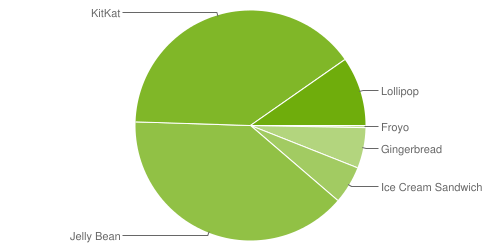
\includegraphics[keepaspectratio, scale=0.8]{Media/Captures/androidUsage.png}
      \caption{Distribución Actual de Versiones Android (Fuente: Google)}
      \label{fig:android_Usage}
    \end{figure}

	Sin embargo existe un problema con la construcción y depuración del código de SwellRT en Eclipse. Android \textbf{limita el número de métodos máximos de una aplicacion a 65K} \cite{ref:android_limit65k} por cuestiones de eficiencia. Para evitar esta limitación, durante el proceso de construcción el SDK de Android utiliza, entre otras, una herramienta llamada \textbf{ProGuard} \cite{ref:android_proguard}. Esta herramienta se encarga de optimizar el código de la aplicacion buscando remover clases que no se utilizan y ofuscando el código para prevenir la ingeniería inversa. En el caso de SwellRT, el código posee un gran número de clases java necesarias para desplegar el servidor y el cliente de la herramienta, por lo que es necesaria dicha optimización de código realizada por ProGuard. El sistema de compilación de aplicaciones de Android tiene dos formas: compilacion de la aplicacion en modo debug (para hacer pruebas cuando todavía se encuentra en fase de desarrollo) y en modo release (la aplicación se encuentra en su versión final y se empaqueta y se firma digitalmente para lanzarla al público). En el caso de Eclipse, ProGuard solo se ejecuta cuando se construye en modo release, por lo que cuando se intenta compilar una aplicación con tantas clases como SwellRT mientras se desarrolla (modo debug) el sistema da error y no se puede compilar el código para probarlo en el emulador. \\[.2cm]

	La solución que encontramos fue desarrollar en Eclipse (por las facilidades que el entorno proporciona para escribir código) pero realizar el proceso de construcción del código por consola de comandos, ya que en este caso sí que se puede compilar la aplicación en modo debug utilizando ProGuard.

	     
    		\subsubsection{Proceso de Construcción por Consola}

		Para construir la aplicación por consola de comandos, Android utiliza la herramienta Apache Ant \cite{ref:ant} para automatizar el proceso de construcción \cite{ref:android_cmd_line}. Es importante asimismo tener definida la variable de entorno JAVA\_HOME con la ruta de acceso al JDK de java instalado en la máquina. Conviene también, por comodidad a la hora de trabajar con la consola, añadir al PATH del sistema las rutas a la carpeta donde esta el SDK de android (/sdk) y dentro de esta ruta añadir asimismo rutas a las carpetas /tools y /platform-tools. \\[.2cm]

Existen dos formas de realizar la construcción en modo debug de una app: \\[.2cm] 

\textbf{1 - Sin tener previamente lanzado un emulador o conectado al ordenador un dispositivo android en modo debug \cite{ref:android_device_setUp}:} \\[.2cm]
 
 	 En este caso es necesario construir la aplicación y luego lanzar el emulador para después instalar la aplicación en él. Para construir la aplicacion en modo debug nos vamos a la carpeta raíz de nuestro proyecto y ejecutamos el siguiente comando: 

 	 \begin{lstlisting}[style=console, numbers=none]
		$ ant clean debug
	 \end{lstlisting}
 	 
 	 Esto nos generará una aplicacion instalable en el directorio /bin del proyecto bajo el formato que Android usa para sus aplicaciones (.apk). El siguiente paso es ejecutar un emulador o conectar un dispositivo android por USB. Para ejecutar un emulador, abrimos otra consola y utilizamos el siguiente comando:
 	 
 	 \begin{lstlisting}[style=console, numbers=none]
		$ android avd
	 \end{lstlisting}
 	 
 	 Lo que nos despliega la herramienta Android Virtual Device Manager (Ver Seccion \ref{sssec:eclipse}) para que elijamos/creemos el emulador que queremos ejecutar. Podemos elegir multitud de parámetros \cite{ref:android_avd_params} para el dispositivo que emula (resolución y tamaño de pantalla, de memoria Ram, elementos hardware emulados, etcétera.) siendo lo más importante elegir un API (versión de Android) que se corresponda con el API que hemos elegido para nuestra aplicación (en nuestro caso API 19). Es recomendable también elegir una imagen del sistema que use un procesador con arquitectura Intel x86, ya que si elegimos la opción por defecto de ARM (los dispositivos móviles actuales usan procesadores ARM) la ejecución del emulador se ralentiza mucho al tener que emular una arquitectura de procesador distinta a la suya (los ordenadores actuales usan arquitectura Intel x86 en su mayoría). Esto únicamente afecta al rendimiento del emulador, la aplicación es independiente de la arquitectura que haya por debajo. \\[.2cm]
 
     Una vez lanzado el emulador/dispositivo móvil, procedemos a instalar la aplicación en él ejecutando el siguiente comando en la primera consola (en la que construimos la aplicacion):
		      	 
 	 \begin{lstlisting}[style=console, numbers=none]
		$ adb install XXXX.apk
	 \end{lstlisting}		
 	 
 	 Siendo XXXX la ruta a donde se encuentra el .apk de la aplicación que previamente hemos construido (/bin). La herramienta ADB (Android Debug Bridge) \cite{ref:android_adb} es la que permite la comunicación entre el proceso de la consola de comandos y el emulador/dispositivo móvil. Es importante destacar que si se tienen varios emuladores/dispositivos moviles en ejecucion/conectados hay que especificar en cual se quiere instalar la aplicación añadiendo al comando lo siguiente: \textbf{-s emulator -YYYY} siendo esto último el identificador del emulador que podemos encontrar en el título de la ventana del emulador. \\[.2cm]
	     
	\begin{figure}[H]
      \centering
	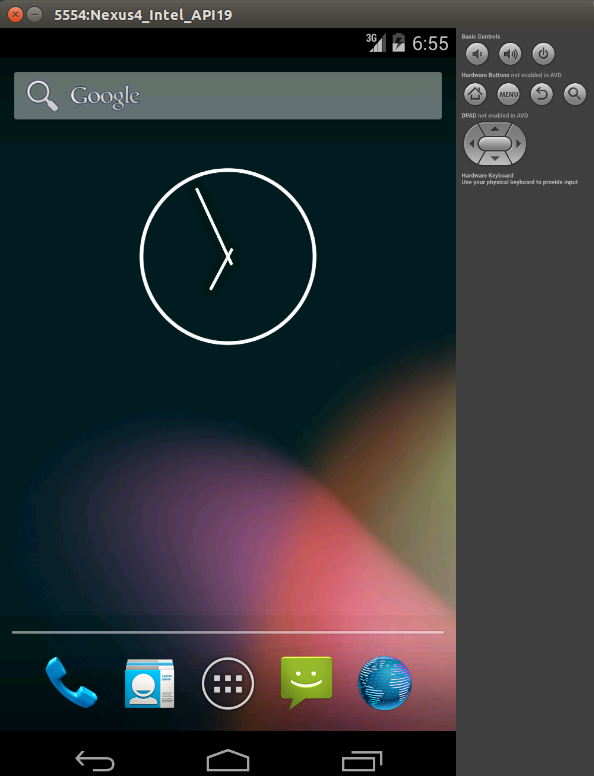
\includegraphics[keepaspectratio, scale=0.3]{Media/Captures/emulator_api_19.png}
      \caption{Emulador Android API 19}
      \label{fig:android_emulator19}
    \end{figure} 
    
    De esta manera podemos probar la aplicación, que será lanzada en el emulador/dispositivo una vez termine su instalación. \\[.2cm]

	\textbf{2 - Teniendo un emulador previamente lanzado (ver sección anterior para ver cómo se lanza) o un dispositivo móvil ya conectado por USB:} \\[.2cm]
	
	En este caso es todavía más sencillo el proceso de construcción. Nos vamos a la carpeta raíz del proyecto  y podemos compilar e instalar la aplicación con un solo comando:

 	 \begin{lstlisting}[style=console, numbers=none]
		$ ant debug install
	\end{lstlisting}	
 	 
 	 Es importante destacar que este comando solo funciona si tenemos un único emulador o dispositivo conectado, de lo contrario habrá que utilizar el método anterior. \\[.2cm]

    
    		\subsubsection{Proceso de Depuración} \label{sssec:debug}
    
    Una vez instalada una aplicación, podemos depurar su código en ejecución usando la herramienta DDMS del ADT en conjunto con la vista de Debug de Eclipse. Pero antes hay que especificar qué aplicación queremos depurar de las que puedan estar instaladas en el dispositivo o emulador. \\[.2cm]

En el caso del emulador debemos lanzar la aplicación llamada “Dev Tools” y abrir el menú “Developer Options”. Dentro de este menú habilitaremos las opciones de “USB debugging” y de  “Wait for debugger”. Además pulsaremos sobre “Select Debug app” y seleccionaremos la aplicación que queremos depurar. \\[.2cm]

En el caso de un dispositivo Android debemos ir a los Ajustes del dispositivo y seleccionar el menú de Opciones de Desarrollador. Aquí habilitamos las opciones de "Depuración de USB"  (si no esta habilitada ya) y de "Esperar al depurador". Además pulsamos donde pone "Seleccione una aplicación para depurar" y elegimos la aplicación que queremos depurar. \\[.2cm]

Una vez hecho esto, cada vez que ejecutemos la aplicacion saldrá un mensaje de advertencia y se quedará esperando a que conectemos un depurador para continuar con su ejecución. Para esto, nos vamos a Eclipse y abrimos la vista de DDMS. Aquí nos aparecerá, entre otras cosas, un espacio con todos los procesos en ejecución en el dispositivo/emulador. Localizamos el proceso de nuestra aplicación y pulsamos sobre el bichillo verde para conectar el depurador a ella. Llegados a este punto la aplicacion continua su ejecución en el emulador y aparece un escarabajo verde al lado del proceso de la app en la ventana de DDMS, que indica que se esta depurando ese proceso. Es entonces cuando podemos abrir la vista de depuración de Eclipse y proceder a trabajar con breakpoints para depurar y estudiar el código con el fin de solucionar errores.

	\subsection{Migración: Identificación y Solución de Problemas}
  
	  El objetivo de esta parte del proyecto es conseguir que el cliente de SwellRT se pueda desplegar en Android para asi conseguir que se conecte al servidor WIAB que tambien incluye. Para ello lo primero que haremos será desplegar el servidor en nuestro ordenador clonando el repositorio de GitHub de SwellRT y siguiendo los pasos descritos en el Readme del proyecto \cite{ref:swellRT_github}. Para comprobar que el servidor se ha instalado correctamente, podemos ejecutarlo por consola (ver Readme) y abrir un navegador web con la dirección http://localhost:9898. Si nos aparece una ventana de Login de WIAB es que ya tenemos un servidor WIAB corriendo en nuestro ordenador. Creamos entonces un usuario y contraseña de prueba. Este paso es importante ya que la aplicación Android intentará conectarse contra este servidor mientras estemos haciendo pruebas de desarrollo. \\[.2cm]
	  
	  A continuación crearemos un proyecto Android en Eclipse e incluiremos en él todas las clases de SwellRT. Uno de los componentes principales de Android a la hora de desarrollar son las \textbf{Actividades} \cite{ref:android_activities}, que representan las pantallas que se le muestran al usuario y que responden a su interacción programáticamente. Por tanto, crearemos una nueva actividad  
	  principal (waveAndroid.java) que se ejecutará al lanzar la aplicación y que por el momento intentará conectarse al servidor especificando por código el usuario y contraseña que hemos creado antes en el servidor. Wave realiza este login contra el servidor usando dos tecnologias: HTTP \cite{ref:http_authentication} y WebSockets \cite{ref:webSocket_ref}.
	  
  
    		\subsubsection{Conexión HTTP}\label{sssec:conHttp}
	
	Wave fue desarrollado para utilizar el protocolo WebSocket para la conexión al servidor, pero esta tecnología necesita realizar una autenticación HTTP previa. Lo primero que haremos será otorgar \textbf{permisos de conexión a internet} a nuestra aplicación. Android utiliza un \textbf{sistema de permisos} \cite{ref:android_permissions} para controlar los privilegios de cada aplicación. Estos permisos se declaran en el \textbf{Manifiesto} de la aplicación \cite{ref:android_manifest}, archivo que declara sus características. Para ello basta con añadir lo siguiente al manifest.xml de la aplicación:
	  
	  \lstset{language=XML, breaklines=true, autogobble=true, basicstyle=\ttfamily\footnotesize}
	  \begin{lstlisting}[frame=single]
	  	<uses-permission android:name="android.permission.INTERNET"/>
	  \end{lstlisting}
	  
	  	 También hay que tener en cuenta que cuando nos encontramos en el emulador no estamos en la misma red que el ordenador en el que trabajamos, por lo que la conexión a la URL http://localhost:9898 no es válida. No obstante, esto tiene facil solución pues \textbf{el emulador de Android define unas direcciones IP de red especiales} \cite{ref:android_netAddress} para este tipo de casos. Basta con sustituir localhost por la direccion 10.0.2.2 para conseguir acceder al servidor WIAB desplegado en el ordenador. La dirección URL sera por tanto: \textbf{http://10.0.2.2:9898}. 
	  
	 Lo siguiente que haremos será ejecutar el código de Login del cliente SwellRT para intentar localizar dónde se lleva a cabo la conexion HTTP. Para ello llamamos desde la actividad principal (WaveAndroid.java) al método startSession() de la clase WaveClient.java pasándole el usuario y la contraseña antes creados.
 
	 Esto provoca un error de ejecución y la aplicación se cierra. Lo siguiente que hacemos es depurar la aplicación (Ver Seccion \ref{sssec:debug}) estudiando el LogCat \cite{ref:android_logcat} (Ver Figura \ref{fig:android_logcat}) para ver dónde se produce el error. Descubrimos que el problema estaba localizado en el método login() de la misma clase, que intentaba realizar una \textbf{petición POST HTTP} al servidor utilizando un \textbf{RequestBuilder} de la librería \textbf{com.google.gwt.http.client}. He aquí el primer problema: la actual conexión utiliza métodos de GWT/Javascript para hacer la petición Post y Android no es compatible con esta tecnología.   
	 
	\begin{figure}[H]
      \centering
	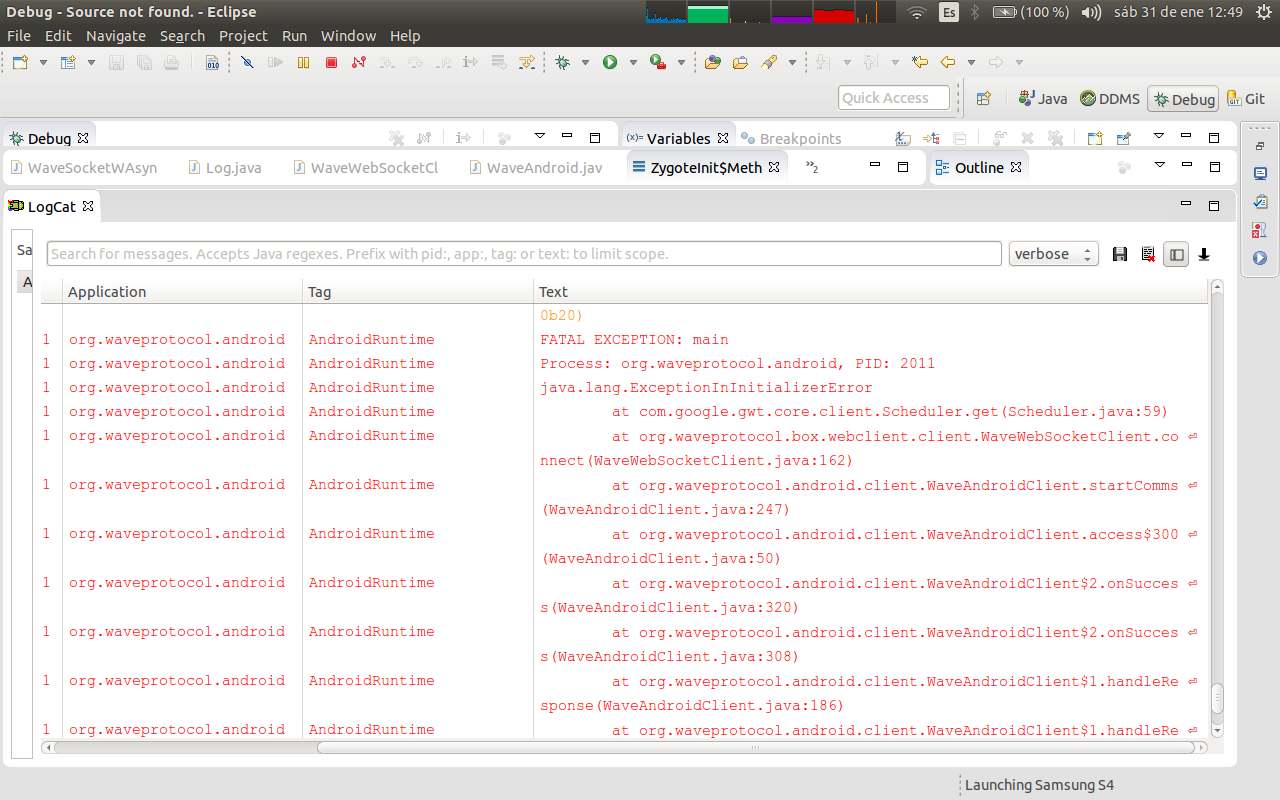
\includegraphics[keepaspectratio, scale=0.3]{Media/Captures/logcat_example.png}
      \caption{Ejemplo de Traza de Error en Logcat}
      \label{fig:android_logcat}
    \end{figure} 
	 
	 Hay por tanto que encontrar una librería similar compatible con Android que construya una petición \textbf{HTTP POST} y la envíe al servidor. La primera opción que valoramos fue utilizar la \textbf{librería HTTP Apache} \cite{ref:apache_http}, incluida en el SDK de Android desde sus primeras versiones. Sin embargo, Google recomienda \cite{ref:http_recommmendations} a partir del API 10 (Android 2.3 "Gingerbread") utilizar la \textbf{librería HttpURLConnection}\cite{ref:android_httpUrlConnection}, también incluida en el API. Por tanto esta última es la que elegimos para la migración. 
	 
	 Se puede ver un esquema simplificado de la nueva estructura del login HTTP en la Sección \ref{ssec:codeHTTP} del Apéndíce.
	  
	 Sin embargo, aquí no acaba el problema. Por cuestiones de usabilidad y de respuesta a la interacción del usuario, Android establece dos reglas para trabajar con el proceso de la actividad que se le esta mostrando al usuario (llamado \textbf{UI Thread}) \cite{ref:android_processes}:
	  
	  \begin{itemize}
	  	\item \textbf{1. No bloquear el UI Thread}
	  	\item \textbf{2. No acceder al UI Thread directamente desde otro Thread}
	  \end{itemize}
	  
	  La conexión a un servidor es un proceso susceptible de durar un tiempo variable según las condiciones de la red, lo cual deja la aplicación en espera hasta que se realiza dicha conexión,  bloqueando el UI Thread. Por tanto, decidimos usar un hilo (Thread) por separado en forma de \textbf{AsyncTask} \cite{ref:android_asynctask} para llevar a cabo la tarea de Login, tal y como recomienda Google hacer para trabajar con conexiones a la red \cite{ref:android_networking}. La ventaja por tanto de usar otro hilo para esto es que la actividad principal no se bloquea.
	  	 
	  Es importante también destacar que la arquitectura de SwellRT y de Wave está planteada de manera que utiliza llamadas asíncronas (callbacks) para notificar al resto de la aplicacion del resultado de los procesos de conexión al servidor, por lo que nuestro AsyncTask tendrá que usar el callback apropiado para notificar del éxito o fracaso de la conexión Http.
	 
	  Se puede ver un esquema del AsyncTask encargado del Login en la Sección \ref{ssec:codeAsynctask} del Apéndíce.
	    
	  Este proceso de conexión Http nos deberá devolver una Cookie que trataremos con el onjetivo de generar un SessionId que será necesario para seguir con la conexión al servidor. \textbf{Llegados a este punto, tenemos un proceso de login Http que hace uso de la librería HttpUrlConnection y de un AsyncTask para realizar esa primera conexión al servidor.} Depuramos la aplicación y comprobamos que efectivamente el login Http se realiza correctamente (la respuesta del servidor tiene código 200). \textbf{Sin embargo la aplicación aún no funciona correctamente, pues se cierra al intentar ejecutar el código que se encarga del siguiente paso de la conexión: conectarse por WebSocket.}    
    
    		\subsubsection{Conexión WebSocket}\label{sssec:conWave}
    
    Para realizar una conexión con el servidor Wave es necesaria una conexión mediante WebSockets\cite{ref:webSocket_ref}, tecnología que permite conexiones bidireccionales y asíncronas entre el servidor y el cliente (recordemos que la conexión en el modelo cliente-servidor tradicional está definida como unidireccional de cliente a servidor), de manera que cualquiera de los dos puede iniciar una conexión con el otro en cualquier momento e intercambiar información con éste. En el caso del protocolo Wave este comportamiento es el deseable, ya que al tratarse de un protocolo de comunicaciones federado en el que cualquiera en la red puede ser cliente o servidor, es importante que la conexión sea bidireccional. Además la asincronía es necesaria ya que para mantener la consistencia en tiempo real \ref{sssec:realTime} hace falta que el servidor que contiene las waves pueda iniciar una conexión con los clientes para notificar los cambios que se produzcan en dichas waves. Por tanto, nuestro cliente Android debe ahora establecer una conexión WebSocket con el servidor WIAB. 
    
    La metodología a utilizar será la misma que para la conexión HTTP, se ejecutará el código de SwellRT para identificar dónde falla y por tanto cómo está estructurada la creación y gestión de WebSockets en la versión GWT.
    
    El cliente SwellRT original realiza esta conexión utilizando una librería llamada Atmosphere \cite{ref:atmosphere}, que proporciona un framework para Java que permite gestionar conexiones WebSocket junto a la conexión HTTP que subyace por debajo. Sin embargo, esta librería se encarga solo de gestionar la conexión, no de crear el WebSocket propiamente dicho. En el caso de SwellRT este WebSocket se crea utilizando la implementación que proporciona GWT llamada también WebSocket (WebSocket.java). Esta clase nos define las funciones básicas que debería tener nuestro WebSocket: \textbf{onOpen()} para establecer la conexión, \textbf{onMessage()} para recibir mensajes por el WebSocket, \textbf{send()} para enviar mensajes y \textbf{onClose()} para cerrar la conexión. Asímismo nuestro Websocket deberá también implementar una serie de callbacks (definidos en la interfaz WebSocketCallback.java) para notificar a la aplicación de la llegada de estos eventos del servidor. Los callbacks son: \textbf{onConnect()}, \textbf{onDisconnect()} y \textbf{onMessage(message)} respectivamente.
	
	Este WebSocket se crea utilizando un \textbf{patrón de diseño Factory}, que abstrae la creación de un objeto de su implementación, de manera que el desarrollador tenga acceso al objeto sin tener que preocuparse de cómo este implementado el WebSocket por debajo (ver WaveSocketFactory.java en SwellRT). En este caso, como ya se ha dicho, con Atmosphere y WebSocket GWT. No obstante, la aplicación no funciona tal y como está hecho en SwellRT ya que android no soporta GWT de forma nativa. Hay que sustituir este código buscando una librería open-source que implemente un WebSocket en Android sobre Atmosphere y que porporcione las mismas funciones básicas descritas en el párrafo anterior.
	
	La solución encontrada fue utilizar wAsync\cite{ref:wAsync_github}, librería proporcionada por Atmosphere para trabajar con Websockets en Node.js, Java y Android. wAsync trabaja creando un socket que responde a eventos diversos, estando entre ellos eventos similares a los utilizados por la versión GWT de SwellRT: \textbf{on(EVENT.name())}, siendo EVENT el nombre del evento al que debe responder. 
	
	Se puede ver un ejemplo sencillo de utilización de wAsync en la Sección \ref{ssec:codewAsync} del Apéndíce.
	
	Como la arquitectura Wave utilizaba el patrón factoria, fue necesario sustituir la clase de WebSocket GWT por una de nueva creación llamada \textbf{WaveSocketWAsync.java}\cite{ref:wave_migration_github} que implementa los métodos de creación y configuración de un Websocket y de callback antes descritos. Asimismo se modificó la clase WaveSocketFactory.java para hacer uso ahora de esta nueva implementación del WebSocket compatible con Android. 
	
	Sin embargo, ejecutamos esta nueva versión de código y nos encontramos con que la librería WAsync incluye dependencias a código que no está presente en la propia librería y que es necesario para crear el cliente AsyncHTTPClient que gestiona la conexión HTTP que subyace por debajo del WebSocket. Concretamente hace falta utilizar un HTTPProvider compatible con Atmosphere, tal y como recomienda hacer wAsync en su wiki\ref{cite:httpProvider_wAsync}. Para ello basta con añadir al proyecto las librerias oportunas (Ver Tabla de dependencias \ref{fig:dependencies_swellRT}) y configurar el cliente segun lo descrito en dicha wiki:
		
	\lstset{language=Java, breaklines=true, autogobble=true, basicstyle=\ttfamily\footnotesize, commentstyle=\color{OliveGreen}, keywordstyle=\color{MidnightBlue}}
	  \begin{lstlisting}[frame=single]	
	  AsyncHttpClientConfig ahcConfig = new AsyncHttpClientConfig.Builder().build();
	  AsyncHttpClient ahc = new AsyncHttpClient(new GrizzlyAsyncHttpProvider(ahcConfig));
	  \end{lstlisting}
      
      Ahora, al ejecutar la aplicación comprobamos que la conexión al servidor se produce correctamente. Para completar esta parte del proyecto solo falta pedir al usuario su user y password, ya que hasta ahora las habiamos especificado a mano en el propio código para realizar pruebas.
	    
    		\subsubsection{Conexión final y Logging}
    
    Para probar que la aplicación migrada es funcional y es capaz de utilizar las características nativas de Android haremos una pequeña y sencilla pantalla de Login que pedirá al usuario la dirección del servidor Wave, un usuario y una contraseña.
    
    En el diseño de aplicaciones Android el componente principal de una app es la Actividad, que se corresponde con la pantalla con la que interactúa el usuario. La interfaz gráfica se usuario (UI) de las pantallas se encuentra separada del código de la aplicación en ficheros xml de Layout\cite{ref:android_layout}. A una Actividad se le especifica cuál es su archivo de layout en su método onCreate(), responsable de la creación de la actividad y sus recursos. 
    
    Creamos una Actividad llamada WaveAndroid.java que haga uso del layout Main.xml, en el cual incluimos tres cajas de texto (llamadas EditText en Android) para que el usuario introduzca los datos. Además guardamos una referencia a estas cajas de texto en la Actividad para poder acceder al texto introducido y pasárselo al método login de Wave que hemos migrado anteriormente.
    
    	\begin{figure}[H]
      \centering
	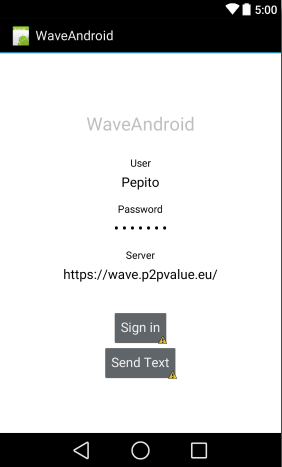
\includegraphics[keepaspectratio, scale=0.6]{Media/Captures/waveAndroidLogin.png}
      \caption{Pantalla de Login de WaveAndroid}
      \label{fig:android_waveLogin}
    \end{figure}
    
    Además decidimos mejorar el sistema de mensajes de Log de la aplicación sustituyendo el framework de la librería SLF4J para Java usada por SwellRT por una versión más reciente desarrollada para Android\cite{ref:slf4j_android}.
        
    Por último instalamos la aplicación en el emulador o el dispositivo móvil y probamos que se nos muestra la pantalla de login anterior. Introducimos los datos del servidor WIAB (en este caso utilizaremos el servidor de P2PValue desplegado para pruebas en https://wave.p2pvalue.eu/), de usuario, contraseña y comprobamos que hemos conseguido el objetivo de esta parte del proyecto: \textbf{nuestro cliente Android realiza el login contra el servidor WIAB correctamente.} 
     
    		\subsubsection{Organización del código: Servicio Android}
    
    Una vez conseguida la conexión al servidor desde Android, decidimos revisar el código para intentar optimizarlo y organizarlo de manera que aprovechara mejor las características de Android y la arquitectura de Wave. Además, el API que permite gestionar el modelo de datos de SwellRT (Ver Sección \ref{sssec:swellRT}) está escrito en java, por lo que es plenamente funcional y compatible con el código de nuestra migración a Android. A continuación hablaremos de los motivos de dicha reorganización.
  
    Como ya se ha comentado anteriormente, el proceso de login se debe hacer en un hilo de ejecución separado del hilo principal o UI Thread, ya que Android no recomienda\cite{ref:android_processes} que tareas que tarden mucho tiempo en ejecutarse (cómo por ejemplo descarga de datos de la red) se ejecuten en el mismo hilo que la interfaz de usuario, pudiendo bloquear dicho hilo y obstaculizando por tanto la interacción del usuario con el dispositivo.
      
    Hasta ahora habíamos utilizado para ello una Actividad que cotenía el AsyncTask \cite{ref:android_asynctask} encargado de ejecutar el código de conexión al servidor en un hilo separado del UI Thread. Sin embargo, tal y como está definida la arquitectura de Wave y de SwellRT, la utilización de callbacks (ver secciones \ref{sssec:conHttp} y \ref{sssec:conWave}) es necesaria para notificar al resto de la aplicación de los eventos relacionados con el intercambio de datos con el servidor. Un AsyncTask ejecuta de una sola vez y de forma asíncrona el código que se le asigne a su método doInBackground(), de manera que una vez que termina su ejecución puede notificar el resultado de la conexión, pero no queda a la espera de otros posibles eventos en el socket (como la recepción de mensajes o la desconexión). Es decir: \textbf{aunque se definan callbacks para esperar los eventos del servidor, el socket no podrá notificarlo porque no existe un hilo que quede a la espera de estos eventos.}

    Por otro lado, cada vez que quisiéramos realizar algún tipo de interacción con el servidor habría que utilizar un AsyncTask específico para ello, lo cual no hace sino añadir más código a la aplicación. Otra desventaja de los AsyncTask en la implementación inicial es que si la Actividad que lo esta ejecutando pasa a segundo plano (por ejemplo si el usuario cambia de aplicación) se detiene el proceso de conexión. 

    Considerando todo esto decidimos utilizar otro componente de Android pensado para ejecutar tareas en background y con la opción de hacerlo de forma independiente de la aplicación: el Servicio\cite{ref:android_service}.

    Un Servicio Android se diferencia de una Actividad en que es un componente que se ejecuta en segundo plano y no proporciona una interfaz de usuario con la que éste pueda interactuar. Un Servicio ejecuta tareas de larga duración (cómo la descarga de datos de la red) a petición de otros componentes de la aplicación que estén \textit{suscritos} (el término utilizado por android es \textit{bind}) a dicho Servicio, a modo de cliente-servidor. De esta manera la Actividad (cliente) que se suscriba al Servicio (servidor) puede interactuar con éste último haciendo peticiones y recibiendo notificaciones cuando el Servicio obtenga resultados. \textbf{Por tanto, podremos acceder a la conexión al servidor desde cualquier punto de la aplicación, solo es necesario que la Actividad en ejecución se suscriba al Servicio para hacerlo}. 
    
    Pero un Servicio se ejecuta dentro del mismo proceso que el UI Thread, por lo que aun así tendremos que utilizar métodos para ejecutar el código que nos interese en otros hilos de ejecución dentro del propio Servicio. De esta manera \textbf{se dividió la reorganización en dos: la conexión Http y la conexión WebSocket.}
    
    Para la conexión HTTP, se decidió utilizar un AsyncTask llamado LoginTask muy similar al ya explicado anteriormente (ver Sección \ref{sssec:conHttp}) pero esta vez definido dentro del propio Servicio y con un callback que notificaba a la aplicación si la conexión se realizaba correctamente. Además, se puso el código de la conexión en una clase aparte llamada WaveHttpLogin.java para tenerlo más organizado. El siguiente es un esquema en forma de Diagrama de Secuencia de la conexión Http:
    
  \begin{figure}[H]
   \centering
	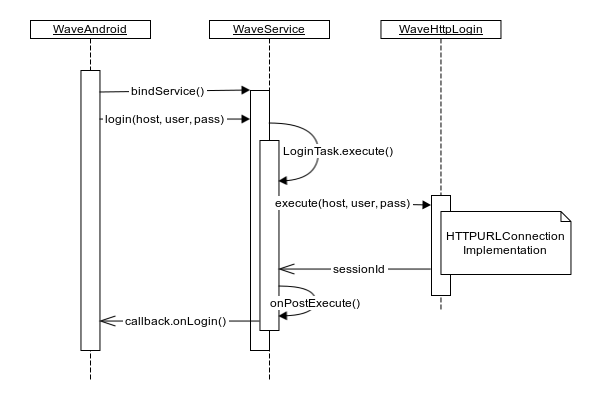
\includegraphics[keepaspectratio, scale=0.6]{Media/Diagrams/loginHttpSequenceDiagram.png}
    \caption{Proceso de conexión Http con Servicio}
   \label{fig:sequenceDiagram_waveHttp}
  \end{figure}
    
    Como vemos, cuando se realiza esta conexión Http la Actividad inicial (WaveAndroid.java) es informada de ello mediante su callback onLogin() para poder notificar al usuario e iniciar la conexión por WebSocket. 
    
    Para dicha conexión se debía buscar una solución que permitiera al WebSocket responder a eventos del servidor (recordemos el funcionamiento de WAsync descrito en la Sección \ref{sssec:conWave}) para, mediante callbacks, informar a la aplicación de dichos eventos. \textbf{La solución final encontrada fue combinar el uso de un Thread y un Handler}. El Thread se encarga de crear el socket y configurar su respuesta a eventos en forma de mensajes, que enviará entonces al Handler, encargado de quedar a la espera de recibir estos mensajes de forma asíncrona y llamar al callback adecuado. Esta imnplementación se puede ver concretamente dentro de la clase WaveSocketWAsync.java, donde se define el Thread llamado WebSocketRunnable y el Handler UIHandler. El siguiente es un esquema en forma de Diagrama de Secuencia de la conexión inicial con WebSocket al servidor Wave:
    
  \begin{figure}[H]
   \centering
	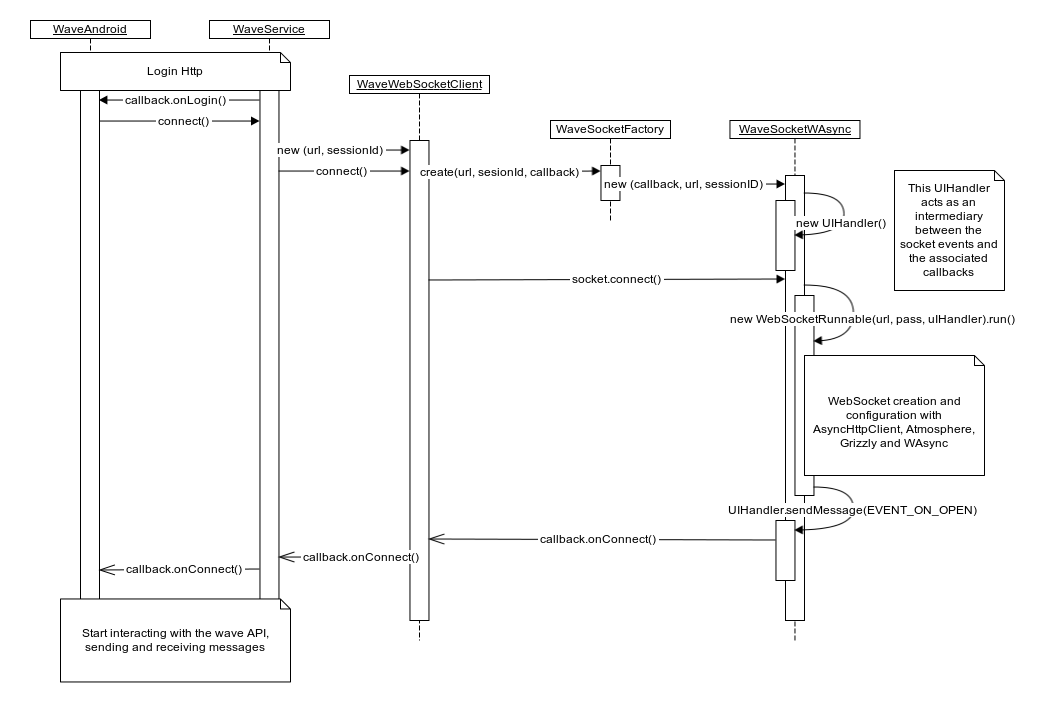
\includegraphics[keepaspectratio, scale=0.43]{Media/Diagrams/waveServerConnectionSequenceDiagram.png}
    \caption{Proceso de conexión WebSocket con Servicio}
   \label{fig:sequenceDiagram_waveWebSocket}
  \end{figure}
     
      Como vemos, cuando se realiza esta conexión al Servidor Wave la Actividad es notificada de ello mediante la propagación de callbacks onConnect() que informan del éxito de la conexión. A partir de este momento el socket informará de la misma forma (mediante el envío de mensajes al UIHandler) de otros eventos que se produzcan, ya sea la recepción de datos o la desconexión por ejemplo. De la misma forma la aplicación podrá enviar datos al servidor, ya que el socket se mantiene en el Servicio. 
       
    \subsection{Dependencias}
    
    El cliente Android de SwellRT migrado y desarrollado en esta parte del proyecto hace uso de las siguientes dependencias con librerías externas a Android:

    \begin{table}[h]
      \footnotesize
      \begin{center}
	\begin{tabular}{ | c | c | m{8cm} | }
	  \hline
	  \textbf{Nombre} & \textbf{Versión} & \textbf{Descripción} \\
	  \hline
	  WAsync \cite{ref:wAsync_github} & 1.4.3 & WebSockets/HTTP Client Library for Asynchronous Communication \\ 
	  \hline
	  AsyncHttpClient \cite{ref:asyncHttpClient} & 1.8.14 & Library that allows Java applications to easily execute HTTP requests and asynchronously process the HTTP responses.\\ 
	  \hline
	  Grizzly-Framework \cite{ref:grizzly} & \multirow{3}{*}{2.3.18} & Core framework for Grizzly applications that provides TCP/UDP transports, memory management services/buffers, NIO event loop/filter chains/filters. \\ \cline{1-1} \cline{3-3} 
	  Grizzly-Http \cite{ref:grizzly} & & HTTP framework that contains the base logic for dealing with HTTP messages on both the server and client sides. \\ 
	  \cline{1-1} \cline{3-3} 
	  Grizzly-WebSockets \cite{ref:grizzly} & & WebSockets custom API for building Websocket applications on both the server and client sides. \\ 
	  \hline
	  slf4j-Android \cite{ref:slf4j_android} & 1.6.1 & Simple Logging Facade for Java: logging framework for Android \\ 
	  \hline
	\end{tabular}
      \end{center}
      \caption{Dependencias de SwellRT-Android}
      \label{fig:dependencies_swellRT}
    \end{table}       
       
    \subsection{Resultado de la Migración} \label{ssec:migrationResult}
    
    Después de todos estos pasos disponíamos de una versión funcional de SwellRT capaz de conectarse al servidor WIAB de forma nativa desde Android. \textbf{El resultado de esto se puede ver en el GitHub de esta parte del proyecto}\cite{ref:wave_migration_github}. El siguiente es un esquema en forma de Diagrama de Clases del resultado final:
    
  \begin{figure}[H]
   \centering
	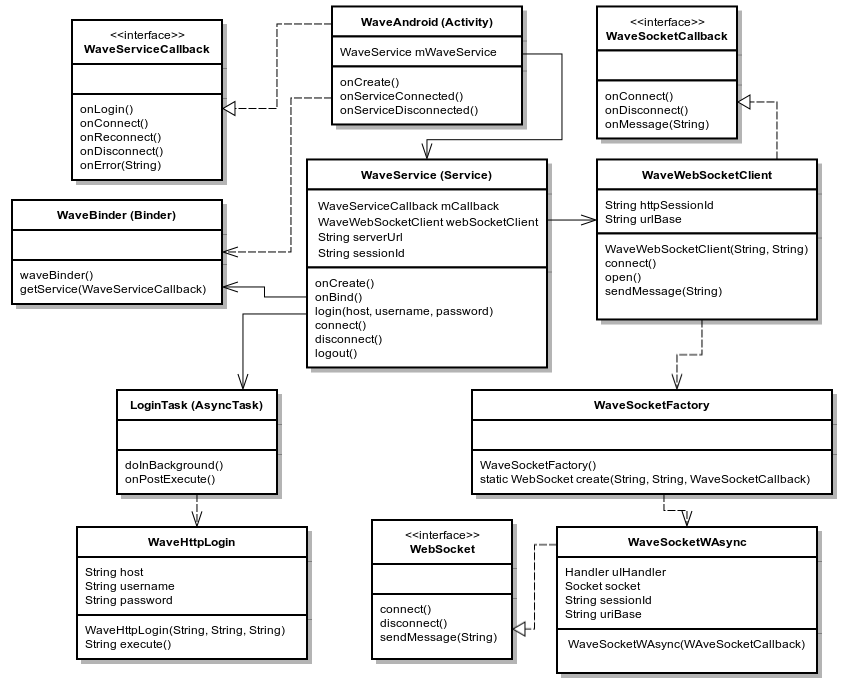
\includegraphics[keepaspectratio, scale=0.5]{Media/Diagrams/waveServiceClassDiagram.png}
    \caption{Esquema de Clases de SwellRT-Android con Servicio}
   \label{fig:sequenceDiagram_waveWebSocket}
  \end{figure}
    
    Solo restaba poner el API de SwellRT encima de lo nuestro para poder acceder y trabajar a nivel de wave con el modelo de datos de SwellRT. De esto se encargó uno de los desarrolladores del proyecto inicial, Pablo Ojanguren, con el cual habiamos trabajado para realizar lo anteriormente descrito.
    
    El API con el cliente de SwellRT adaptado a Android, con el cual trabajaremos en la siguiente parte del proyecto para crear una aplicación Android que haga uso de ello, se encuentra en el GitHub de SwellRT\cite{ref:swellRT_android_github}. 


\section{Diseño de la Aplicación: Diseño Guiado Por Objetivos}

Para elaborar el diseño de la aplicación, nos hemos basado en la metodología del Diseño Guiado por Objetivos (\textbf{DGO} o \textit{Goal-Directed Design}), que implementa el proceso de la Ingeniería de la Usabilidad propuesto por Alan Cooper \cite{ref:bookAlanCooper}. Este proceso constará de las siguientes fases:

\begin{enumerate}

\item \textbf{Investigación}

Esta fase consistirá en la realización de estudios para obtener datos cualitativos sobre los usuarios y/o reales de la aplicación y cuáles son sus necesidades. Se realizarán tareas para comprender a los usuarios, saber sus inquietudes y lograr empatía. A lo largo de esta fase se irán identificando patronos de comportamiento que sugerirán los objetivos y motivaciones del usuario. Por último se realizarán estudios de mercado, revisiones y auditorías que ayudarán al diseñador a comprender el dominio, el modelo y las restricciones técnicas que el sistema debe cumplir.

\item \textbf{Modelado}

A lo largo de esta fase se utilizarán los datos provenientes de la fase previa para crar los modelos del dominio y los usuarios. En esta parte se crearán las \textit{personas}, aquetipos de usuarios que contienen información sobre obejtivlos, motivaciones y comportamientos de los usuarios con el sistema. El resultado final de esta fase serán los tipos de \textit{persona} que representarán a los usuarios del sistema, y que más adelante serán utilizados fases para proporcionar algún tipo de \textit{feedback}.

\item \textbf{Definición de Requisitos}

Durante esta fase se utilizarán las personas y los datos de la fase anterior, para crear los \textit{escenarios} de contexto e identificar los requisitos o necesidades del usuario. Estos requisitos serán definidos en tres componentes: objeto, acciones y contexto. También se definirán requisitos relacionados con el negiocio, la apclicación, requisitos técnicos, etcétera.

\item \textbf{Definición del framework de Diseño}

En esta fase se creará el concepto geenral del sistema, definiendo los comportamientos y diseño visual. Identificaremos el \textbf{framework de interacción}, como un concepto de diseño estable que define la estructura del sistema a partir de patrones y principios de diseño. Por último, se definirá el \textit{framework visual}, como el aspecto visual de la aplicacion (diseño, tipografía, colores, iconos, etcétera).

\end{enumerate}

Queremos insistir eso sí en que únicamente nos hemos basado en esta metodología para seguir el proceso del diseño de la aplicación. No seguiremos todas las fases de esta metodología al pie de la letra ya que el alcance en tiempo de este proyecto escapa a una metodología tan formal y laboriosa (que implica gran cantidad de pruebas y procesos) como esta.

\subsection{Investigación}

\subsubsection{Intención Inicial: Prototipo básico}  

Vivimos en una época donde la política parece estar de moda. Esto puede ser debido al cabreo general que muestra la ciudadanía frente a gobiernos conservadores, situaciones de austeridad provocada por la crisis económica, el nacimiento de nuevas fuerzas políticas, …, pero sobre todo las numerosas citas electorales a las que seremos citados en 2015. Por tanto, el proyecto podría ponerse a prueba en un escenario real durante la campaña de las elecciones generales previsiblemente convocadas durante el último trimestre del 2015.

\underline{Programas electorales}

La intención fundamental de la aplicación es llevar los programas electorales a los bolsillos de los ciudadanos y generar interés en participar más activamente en la política, ya sea emitiendo opiniones sobre dichos programas o elaborando nuevas propuestas. Vivimos en una sociedad digital, donde cada vez son más las personas que utilizan sus smartphones para realizar todo tipo de tareas en su vida cotidiana.

En los últimos años las diferentes formaciones políticas han subido sus programas electorales a un documento en formato PDF que suele estar disponible para su descarga en su página web. Este documento tiene generalmente una gran extensión (los hay de 200 páginas), lo cual no hace sino dificultar que las personas se animen a leerlo. Por ello pensamos que una aplicación que pudiera visualizar las principales secciones de los programas políticos podría ser especialmente útil para acercar los programas a los electores.

Además también intentariamos darle una estructura a estos programas, de manera que el usuario pudiera navegar por ellos a nivel de Sección, a diferencia del método actual de leer un "macro-documento" en PDF. Así, la gente podría opinar sobre los programas políticos a nivel de sección mediante acciones familiares para ellos: "Me gusta", "No me gusta" y realizar "Comentarios". Añadimos también una acción de "No lo entiendo" que pensamos que seria util para indicar cuándo la redacción de la sección era de significado difuso.

En definitiva, queríamos crear un espacio donde poder informarse sobre las distintas ofertas electorales y poder debatir sobre las propuestas que propone cada formación política, todo ello en forma una aplicación que podremos consultar en cualquier momento. 

\underline{Propuestas y Wave}

Por otro lado,y en línea con los últimos movimientos políticos ciudadanos, pretendíamos crear también un portal de propuestas ciudadanas en el móvil. Los usuarios podrían visualizar las propuestas de otros usuarios y tener la posibilidad de crear nuevas propuestas. Además, como queríamos aprovechar las características de la migración de Wave previamente desarrollada, pensamos en la posibilidad de elaborar estas propuestas de forma colaborativa y en tiempo real entre muchos usuarios.

Actualmente existen multitud de portales (en su gran mayoría web) donde la ciudadanía puede expresar su opinión, pero creemos que la integración de una aplicación donde puedan situarse las opiniones de los partidos políticos (en forma de sus programas) y la actividad ciudadana (en forma de propuestas), genera una nueva manera de tratar la política en los medios sociales.

También pensamos en la posibilidad de categorizar el contenido de la aplicación (Programas y Propuestas) por temas, para proporcionar filtros a la hora de navegar por dicho contenido. Sin embargo no teníamos muy clara la elección de temas, asi como si debiamos darle al usuario la posibilidad de crear nuevos temas o dar nosotros unos temas preestablecidos.
 
Una vez pensada la intención y los principales objetivos de la aplicación, procedimos a realizar unos primeros prototipos en papel de nuestra idea y a implementar un prototipo básico en el móvil (Ver Sección \ref{ssec:protoetctypes}) que mostraba programas políticos estructurados y permitía navegar a nivel de Sección por ellos para leer y emitir opiniones (likes, dislikes, comentarios, etcétera.).  

\subsubsection{Hipótesis de personas}

Para identificar a los usuarios objetivo, tenemos que encontrar a miembros representativos de esos usuarios y animarlos a que participen en nuestra investigación. Para ello reuniremos una serie de características básicas que el usuario deberá cumplir para poder aportarnos los objetivos funcionales de la aplicación. Estas son algunas de las caracaerísticas deseadas:

\begin{itemize}
\item \textbf{Edad}: Entre 16 y 65 años.
\item \textbf{Sexo}: Indiferente.
\item \textbf{Profesión}: Indiferente.
\item \textbf{Aptidudes deseables}: Activismo social, cociencia política, trabajo colaborativo, ... .
\item \textbf{Habilidades técnicas}: Usuario con experiencia media en uso de aplicaciones móviles.
\end{itemize}

Simplificando el tipo de persona que queremos encontrar, lo dividiremos en dos tipos de persona. Por un lado buscaremos al activista social, activo en movimientos sociales, participación en portales con carácter social, etcétera. Mientras que por otro lado buscaremos una persona que muestre cierto interés en el mundo de la política, pero que no participe en moviimentos sociales. Finalmente pudimos contactar con dos miembros de Labodemo \cite{ref:labodemo}, una organización que se dedica al desarollo de nuevas formas de participación ciudadana. Este perfil cubiría en caso del activista social, mientras que para el tipo de persona entendido de la política pero no tan involucrado, escogimos a Javier de la Cueva \cite{ref:jdelacueva}.

El siguiente paso sería estudiar la viabilidad de esta aplicación entrevistando a las personas seleccionadas para realizar una investigación sobre sus necesidades prácticas. Por otra parte también sería útil enseñarles los prototipos básicos que manejábamos para verificarlos. Entendimos que el tipo de persona con el que nos entrevistáramos debía de estar relacionado de alguna manera con el mundo de la política, pues nada mejor que hablar con gente ya interesada en dichos temas para orientarnos por el buen camino.

A continuación detallamos las entrevistas que realizamos en la investigación:

\subsubsection{Entrevista con Labodemo}

Tuvimos la oportunidad de mantener una conversación con dos miembros de Labodemo \cite{ref:labodemo}, en la que aprovechamos para mostrarles un prototipo de la aplicación que estábamos desarrollando. Ambos tenían experiencia en el desarrollo de plataformas de participación ciudadana en Internet: fueron los responsables del desarrollo de los portales de participación del partido político Podemos y la candidatura ciudadana de unidad popular Ahora Madrid.

En ese momento nuestro prototipo móvil se limitaba únicamente a mostrar las diferentes secciones de cada programa, lo cual les pareció útil, aunque no lo suficiente como para atraer a una cantidad considerable de usuarios. Conforme a su linea de trabajo habitual, eran más partidarios de dar a los usuarios la posibilidad de realizar Propuestas además de ver Programas políticos. Les comentamos entonces que antes de hablar con ellos ya habíamos planteado desarrollar Propuestas colaborativas en tiempo real aprovechando la tecnología de Wave. Pero ellos no eran partidarios de esta opción, ya que según ellos acabaría siendo caótico tener tanta gente editando la misma propuesta de cara a generar contenido útil. 

Dándole una vuelta a la categorización del contenido, nos sugirieron que para atraer a usuarios, debíamos considerar la posibilidad de integrar en la aplicación a colectivos sociales que generaran y categorizaran dicho contenido. No eran partidarios de que dieramos nosotros ciertas temáticas preestablecidas, pues debido a la variedad de redaccion en los distintos programas sería dificil identificar temáticas que incluyeran a todos los programas y probablemente acabariamos excluyendo temas. Así, serían los colectivos los que se encargaran de "tematizar" el contenido de la aplicación. Por ejemplo: un grupo de animalistas podría tener un espacio en la aplicación donde poder crear sus propias propuestas, e incluso hacer comparativas de lo que proponen los diferentes programas sobre los animales. 

De esta manera, y en relación a la aproximación a los foros tradicionales, se planteó la idea de crear "Hilos": elementos "temáticos" que agruparan en un solo sitio Secciones y Propuestas que hablaran sobre un determinado tema. Estos hilos serían también generados por dichos colectivos.

Esto sería útil también para usuarios que buscaran información sobre un determinado tema. Por ejemplo: un usuario poco activo, que resulta ser profesor, podría buscar un colectivo de profesores y ver las Propuestas que se llevan a cabo o visualizar una comparativa respecto las medidas de educación de los diferentes programas políticos.

Nos insistieron mucho en el tema de las comparativas. Sería de gran utilidad que la aplicación tuviera una parte de comparativas en la que los usuarios pudieran comparar los programas políticos en vez de leerlos sección por sección. Resultaría de gran interés a un autónomo visualizar las medidas que proponen los diferentes partidos políticos para los autónomos. Pero estas comparativas no podría realizarlas cualquiera, por lo que deberían realizarlas periodistas o expertos que hubieran realizado algún tipo de comparativa similar anteriormente. Nos sugirieron contactar con periodistas o colectivos que hubieran publicado algún tipo de comparativa en cuanto a programas o medidas, para obtener algún tipo de ayuda o consejo a seguir.

\subsubsection{Conclusión}

\underline{Puntos positivos}:

\begin{itemize}
 \item Nueva forma de participación ciudadana de cara a las elecciones.
 \item Métodos alternativos para discutir propuestas, partidos, programas, etcétera.
 \item Ligar propuestas a programas concretos.
\end{itemize}

\underline{Puntos negativos}:

\begin{itemize}
 \item Visualizar un programa electoral en el móvil puede no resultar demasiado interés para los usuarios.
 \item Desarrollar propuestas colaborativas en tiempo real no maniene una estabilidad en la aplicación.
 \item La aplcación debería desarrollarse en otras plataformas móviles y de escritorio.
\end{itemize}

\underline{Puntos a tener en cuenta}:

\begin{itemize}
 \item Dejar libertad a usuarios y colectivos creando sus propias categorías o hilos como ''Espacios'' que puedan elaborar segun sus intereses y generar contenido para la aplicación.
 \item Desarrollar comparativas por secciones, temas o partidos. De tal forma que un usuario pueda visualizar las diferencias de aquellos temas que le preocupan.
 \item Contactar con colectivos, asociaciones y/o periodistas que anteriormente hayan elaborado comparativas entre programas políticos en puntos concretos
\end{itemize}

\subsubsection{Entrevista con Javier de la Cueva}

La entrevista con Javier de la Cueva resultó bastante productiva. Ya le conocíamos de algunas conferencias que impartió en la facultad. Javier es abogado y doctorado en Filosofía, estando especializado en temas relacionados con tecnología, Internet y propiedad intelectual. Además, en sus últimas conferencias Javier habla sobre acciones micropolíticas \cite{ref:manualCiberactivista}. Estas acciones definen la capacidad que tienen los ciudadanos para realizar aportaciones a la sociedad, el estado o el gobierno que favorezcan la participación ciudadana en una democracia participativa.

Representar los programas electorales en una aplicación móvil le pareció algo interesante y necesario para la sociedad actual. Si bien casi nadie hace el esfuerzo de visualizar un programa electoral en PDF, utilizar una herramienta que facilita el acceso al programa por secciones podría ser una nueva forma de incentivar su lectura y ayudar a fomentar la participación ciudadana en política. 

Además nos sugirió la posibilidad de desarrollar una Hemeroteca de programas electorales. De esta forma cualquiera podría consultar los programas de los anteriores gobiernos y comprobar si se cumplieron los objetivos del programa, así como comparar programas de distintos años entre sí, 

Pero si en algo nos insistió Javier, fue en la importancia de categorizar el contenido de la aplicación. Un usuario que no tenga conocimientos sobre diversos temas, se encontraría más cómodo si pudiera visualizar las diferentes partes de un programa o las propuestas ciudadanas por categorías o temas generales. Ya que dejar libertad a los usuarios para crear categorías personalizadas podría ser algo negativo para usuarios inexpertos o con pocos conocimientos sobre temas específicos.

Por último, centrándonos en las Propuestas ciudadanas, surgió la idea de elaborar propuestas que tuvieran una especificación concreta. Es decir, a parte de tener una idea de propuesta y redactarla, esta propuesta debería ir acompañada de los recursos que serían necesarios y sobre todo cómo se llevaría a cabo de una forma aproximada. También resultaría interesante definir un pequeño presupuesto de lo que conllevaría realizar la propuesta o cómo se podría financiar. Así evitaríamos una elaboración de propuestas más real, evitando un listado de propuestas infinito sin planterase cómo se llevarían a cabo o cómo se financiarían.

\subsubsection{Conclusión}

\underline{Puntos positivos}:

\begin{itemize}
  \item Llevar los programas políticos de una forma más atractiva a la ciudadanía es algo esencial en la actualidad.
  \item Categorizar las secciones de los programas políticos para que se puedan explorar por temas.
  \item Incluir los recursos necesarios que hacen falta para llevar una propuesta a cabo.
\end{itemize}

\underline{Puntos negativos}:

\begin{itemize}
  \item Tratar de convertir la aplicación en un \textit{foro} inconscientemente.
  \item Dejar libertad a la hora de crear categorías específicas o hilos puede generar confusión entre los usuarios. 
\end{itemize}

\underline{Puntos a tener en cuenta}:

\begin{itemize}
  \item Desarrollar categorías semanales en función de las novedades o actualidad política.
  \item Añadir la posibilidad de solicitar la ayuda de expertos sobre un tema para elaborar una propuesta.
  \item Crear una emeroteca de programas políticos para realizar análisis sobre el cumplimiento de los programas en legislaturas pasadas.
  \item Informar sobre la legilación actual cuando visualicemos una propuesta o sección de un porgrama que quiera mejorar o cambiar la legislación actual.
\end{itemize}

\subsection{Modelado de Personas}

Las \textit{personas} son una herramienta de diseño y ayuda al diseño de la aplicación. El objetivo es centrar el diseño en este tipo de persona, para lograr los objetivos a la hora de utilziar un sistema. La \textit{persona} será nuestro modelo, una descripción detallada de un individuo imaginario que representa a un grupo de usuarios a los que va destinada la aplicación. Es una representación ficticia pero desarrollada con gran detalle, que será fruto de los datos recogidos en la investigación previa de la fase anterior.

En esta fase definiremos el tipo de persona que interactuará con nuestra aplicación. Para ello hemos identificado dos tipos de personas primarias; un \textbf{activista social} y un \textbf{ciudadano} de a pie que forme parte del electorado.

\textbf{- Activista social, 16 años en adelante}

\underline{Actividad:}

\begin{itemize}
\item Estudia, trabaja o realiza otras actividades de voluntariado.
\item Frecuenta asambleas, participa en diferentes movimientos sociales y está al día de la actualidad política.
\item Utiliza redes sociales para comunicarse con otros colectivos, acudir a asambleas, promover ideas u otras actividades relacionadas con la política y el activismo social.
\end{itemize}

\underline{Otros:}

\begin{itemize}
\item Desconoce las ideas que proponen algunos partidos 
\item Le gusta aportar nuevas soluciones a la sociedad.
\end{itemize}

\textbf{- Ciudadano de a pie, 18 años en adelante}

\underline{Actividad:}

\begin{itemize}
\item Estudia, trabaja o realiza otras actividades de voluntariado.
\item Es distante al mundo de la política, concibe ciertos temas pero no los conoce en profundidad.
\item Visita diferentes medios de comunicación para enterase de la actualidad.
\item Utiliza redes sociales para compartir contenidos con sus amigos o establecer nuevas amistades.
\end{itemize}

\underline{Otros:}

\begin{itemize}
\item Desconoce por completo los programas electorales. 
\item Tiene cierta indecisión a la hora de acudir a las urnas, no sabe que propone cada partido.
\end{itemize}

\subsection{Definición de personas}

En las figuras \ref{fig:studentPerson} y \ref{fig:activistPerson} se exponen una serie de personas ficticias que podrían representar en la vida real los tipos de \textit{persona} a la que va dirigida la aplicación.

	\begin{figure}[!]
      \centering
	
\includegraphics[keepaspectratio, scale=0.45]{Media/Captures/person1.png}
      \caption{Estudiante universitario}
      \label{fig:studentPerson}
    \end{figure}
    
	\begin{figure}[!]
      \centering
	
\includegraphics[keepaspectratio, scale=0.45]{Media/Captures/person2.png}
      \caption{Activista político}
      \label{fig:activistPerson}
    \end{figure}


\subsection{Definición de Escenarios y Requisitos}

En esta sección se definirán los posibles escenarios que puedan surgir en la aplicación. La idea es situarnos en un escenario real que pudera ocurrir en cualquier momento a lo largo del día, para detallar la solución al problema. En cada uno se especificarán los requisitos necesarios para solventar el problema o los pasos a seguir para lograr el objetivo. Diferenciaremos los términos de \textbf{acción}, como la actividad inmediata que requiere la solución. El \textbf{objeto}, como el sujeto principal del escenario. Y por último definimos \textbf{contexto} reflejando el objetivo final del requisito.

\textbf{Escenario I}

Se acercan las elecciones municipales y Juan aún no ha decidido a qué partido va dar su voto. No conoce las propuestas que ofertan los partidos a la ciudadanía y tampoco se fía mucho de lo que dicen los medios de comunicación.

Juan coge su móvil y visualiza los diferentes programas electorales por categoría, seleccionando la categoría de educación que es la que más le afecta a él personalmente. La aplicación le muestra un listado de las secciones donde lso diferentes partidos hablan de las medidas que van a tomar en torno a la educación.

\underline{Requisitos:}

\begin{enumerate}
\item Visualizar (acción) las diferentes categorías (objeto), para ver las secciones de los programas de una determinada categoría (contexto).
\item Mostrar(acción) un listado de todas las secciones de los programas de los partidos  políticos (objeto) en función de la categoría seleccionada por el usuario (contexto).
\end{enumerate}

\textbf{Escenario II}

Pablo es un empleado sanitario de Hospital Clínico de Madrid preocupado por la gestión de los hospitales públicos. Parece que la situación no está muy controlada, por lo que quisiera saber que propuestas o alternativas propone la ciudadanía para mejorar la situación actual.

A través de su móvil puede explorar las diferentes propuestas por categorías. Eligiendo la categoría de sanidad, le aparece un listado de las últimas propuestas desarrolladas por la ciudadanía.

\underline{Requisitos:}

\begin{enumerate}
\item Visualizar (acción) el listado de propuestas (objeto), clasificados por la categoría seleccionada por el usuario (contexto).
\item Mostrar (acción) la propuesta (objeto), seleccionada por el usuario para que pueda puntuarla y/o comentarla (contexto).
\end{enumerate}

\textbf{Escenario III}

Lara es una profesora de un colegio de la Comunidad de Madrid. Se acercan las vacaciones de verano y muchos niños se quedarán sin acceso a comedor. Lara está planteándose cómo elaborar una propuesta ciudana para abrir los colegios en horario no lectivo y que todos los niños tengan derecho a comedor en los meses de verano. Lara no es una experta en gestión pública ni sabe cómo llevar a cabo la propuesta.

Para ello, Laura comienza a desarrollar una propuesta ciudadana en la aplicación, explicando la base de la propuesta. Al no saber cómo financiarlo, deja la propuesta abierta para que la comunidad la pueda ayudar a desarrollarla.

\underline{Requisitos:}
\begin{enumerate}
\item Agregar (acción) una nueva propuesta (objeto) rellenando los principales campos del formulario (contexto).
\item Publicar (acción) la propuesta (objeto) como una propuesta colaborativa para editar (contexto)
\item Mostrar (acción) la propuesta (contexto) en la lista de propuestas colaborativas para que puedan colaborar otros usuarios (contexto).
\end{enumerate}

\textbf{Escenario IV}

Fran es un periodista de un periódico digital. Se acercan las elecciones y está redactando un pequeño artículo acerca de los programas de algunos partidos políticos. Necesita acceder a los programas compeletos de los partidos y visualizar las secciones que le resulten de interés para comentarlas en su artículo.

Accediendo a la aplicación, Fran puede seleccionar los programas de todos los partidos que se presentan a las elecciones. Listando el índice del programa y accediendo a sus secciones.

\underline{Requisitos:}

\begin{enumerate}
\item Visualizar (acción) todos los partidos (objeto) que se presentan a las elecciones (contexto).
\item Seleccionar (acción) un partido polítco (objeto) para visualizar el programa electoral (contexto).
\item Listar (acción) el índice (objeto) de secciones del programa seleccionado (contexto).
\item Visualizar (acción) la sección (objeto) del programa seleccionado por el usuario (contexto).
\end{enumerate}

\subsection{Framework de diseño} \label{ssec:prototypes}

En esta sección detallaremos todos los aspectos relacionados con el desarrollo del aspecto visual y la interacción con la aplicación. Se utilizarán los escenarios y requisitos definidos en la fase anterior para crear los bocetos y prototipos interactivos. Detallaremos los prototipos desarrollados en papel, algunos prototipos intermedios y el prototipo final de la aplicación presentado.

\subsubsection{Framework de interacción}

Para definir el Framework de interacción realizaremos un proceso de seis etapas:

\textbf{Factor de forma, postura y métodos de entrada}

La aplicación será visualizada en un smartphone bajo el sistema operativo Android (con API 15 como mínimo), con tamaños de pantalla entre 3,5 y 6 pulgadas. Que pueda visualizarse en interiores y exteriores.

La \textbf{postura} será \textbf{temporal}. El usuario puede utilizarlo en periodos de tiempo muy breves como puede ser la consulta de alguna sección, propuesta o dar su valoración. Elaborando una propuesta o participando en el desarrollo de una, el usuario necesitará algo más de tiempo, pero seguirá utilizando funciones básicas. Propias de una postura temporal. \\[2cm.]

\textbf{Elementos y datos funcionales} 

\underline{Elementos de datos}:

\begin{itemize}
 \item Programa político
 \begin{itemize}
  \item \underline{Atributos}: partido, programa, secciones, índice, temas.
  \item \underline{Relaciones}: partido-programa, índice-sección.
 \end{itemize}
\end{itemize}

\begin{itemize}
 \item Temas
 \begin{itemize}
  \item \underline{Atributos}: categoría, programa, sección, partido, propuesta.
  \item \underline{Relaciones}: categoría-programa, categoría-propuesta, partido-sección.
 \end{itemize}
\end{itemize}

\begin{itemize}
 \item Propuestas Ciudadanas
 \begin{itemize}
  \item \underline{Atributos}: propuesta, categoría, usuario.
  \item \underline{Relaciones}: propuesta-usuario, propuesta-categoría.
 \end{itemize}
\end{itemize}

\begin{itemize}
 \item Propuestas Colaborativas
 \begin{itemize}
  \item \underline{Atributos}: propuesta, categoría, usuario, edición colaborativa.
  \item \underline{Relaciones}:  usuario-propuesta, propuesta-categoría.
 \end{itemize}
\end{itemize}

\underline{Elementos funcionales}:

 \begin{itemize}
  \item Visualizar los partidos políticos que se presentan a las elecciones.
  \item Mostrar el índice de cada programa político.
  \item Mostrar, valorar y debatir las secciones de los programas políticos.
  \item Visualizar categorías por temas, distinguiendo entre propuestas y secciones de programas.
  \item Mostrar, valorar y debatir las propuestas de los usuarios.
  \item Crear una nueva propuesta en una categoría.
  \item Mostrar las propuestas colaborativas y participar en su desarrollo.
  \item Crear una nueva propuesta incompleta para desarrollarla de forma colaborativa.
 \end{itemize}

\textbf{Grupos funcionales y jerarquías}

Pantalla principal de la aplicación. Grupos de elementos funcionales que contiene:

\begin{itemize}
 \item Lectura y valoración de Programas políticos.
 \begin{itemize}
  \item Visualizar programas políticos.
  \item Ver secciones de programas.
  \item Visualización, valoración y debate de secciones de programas políticos.
 \end{itemize}
\end{itemize}

\begin{itemize}
 \item Clasificación de secciones de programas y propuestas ciudadanas por categorías.
 \begin{itemize}
  \item Ver secciones de programas políticos por tema.
  \item Ver propuestas ciudadanas por tema.
 \end{itemize}
\end{itemize}

\begin{itemize}
 \item Lectura, valoración y creación de Propuestas Ciudadanas.
 \begin{itemize}
  \item Ver propuestas ciudadanas.
  \item Valorar y debatir propuestas ciudadanas.
  \item Creación de propuesta ciudadana.
 \end{itemize}
\end{itemize}

\begin{itemize}
 \item Lectura, colaboración y creación de Propuestas Colaborativas.
 \begin{itemize}
  \item Visualizar las propuestas ciudadanas en desarrollo.
  \item Crear una propuesta colaborativa.
  \item Colaborar en el desarrollo de una propuesta.
 \end{itemize}
\end{itemize}

\textbf{Boceto del framework de interacción}

El proceso de desarrollo de bocetos se ha realizado en espiral, de tal forma que una vez que identificábamos una determinada funcionalidad, la representábamos en un mockup a papel para debatirlo y discutirlo en las entrevistas. A continuación trasladábamos el mockup a un prototipo de alto nivel desarrollado en Android. Para las siguientes implementaciones que añadían nueva funcionalidad el proceso era el mismo:

\begin{enumerate}
 \item Desarrollo de un boceto a papel identificando los elementos funcionales.
 \item Definir la interacción a través de la herramienta POP \cite{ref:pop}.
 \item Implementar un prototipo de mayor fidelidad en Android. 
\end{enumerate}

  \begin{figure}[h]
   \centering
	\includegraphics[keepaspectratio, scale=1]{Media/Captures/prototypesDiagram.png}
    \caption{Modelo de desarrollo de los prototipos.}
   \label{fig:sequenceDiagram_waveWebSocket}
  \end{figure}
  
De esta forma tuvimos que dar un total de tres vueltas a nuestro modelo en espiral para completar el desarrollo.

\begin{enumerate}
 \item \textbf{Programas Políticos}
 
 Estos fueron los primeros bocetos que definían la interacción de la visualización de los programas políticos:
 
 	\begin{figure}[H]
        \centering
        \begin{subfigure}[b]{0.3\textwidth}
                \includegraphics[width=\textwidth]{Media/Captures/prot1_1.png}
                \caption{Protipo en papel.}
                \label{fig:quipDesktop}
        \end{subfigure}
        ~
        \begin{subfigure}[b]{0.3\textwidth}
                \includegraphics[width=\textwidth]{Media/Captures/prot1_2.png}
                \caption{Protipo interactivo en POP.}
                \label{fig:quipText}
        \end{subfigure}
        ~
        \begin{subfigure}[b]{0.3\textwidth}
                \includegraphics[width=\textwidth]{Media/Captures/prot1_3.png}
                \caption{Implementación en Android.}
                \label{fig:quipComments}
        \end{subfigure}
        \caption{Primeros protitipos sobre programas electorales.}\label{fig:protPrograms}
	\end{figure}
	
\underline{Elementos del protitipo en papel}:

\begin{enumerate}
 \item Partidos políticos
 \item Programas políticos
 \item Índice de programas políticos
 \item Secciones de proramas políticos
\end{enumerate}

\underline{Funcionalidades del protitipo interactivo}:

\begin{enumerate}
 \item Visualizar la lista de partidos políticos.
 \item Seleccionar un programa político.
 \item Navegar por el índice de un programa polítco.
 \item Visualizar secciones de un programa, valorarla y comentarla.
\end{enumerate}

\underline{Implementación en Android}:

\begin{enumerate}
 \item Descargar la lista de partidos políticos del servidor.
 \item Descargar el programa seleccionado.
 \item Navegar por el índice del programa.
 \item Descargar el contenido de las secciones.
 \item Añadir comentarios al servidor.
 \item Modificar parámetros sociales en el servidor (like, dislike, views, etc).
\end{enumerate}

\item \textbf{Bocetos de Propuestas Ciudadanas}

A partir de lo desarrollado hasta el momento, se procedió a diseñar las propuestas en la aplicación. Manteniendo la coherencia con el diseño anterior, contuamos desarollando los protitipos que añadían la funcionalidad de las propuestas ciudadanas.

	\begin{figure}[H]
        \centering
        \begin{subfigure}[b]{0.3\textwidth}
                \includegraphics[width=\textwidth]{Media/Captures/prot2_1.jpg}
                \caption{Protipo en papel.}
                \label{fig:quipDesktop}
        \end{subfigure}
        ~
        \begin{subfigure}[b]{0.3\textwidth}
                \includegraphics[width=\textwidth]{Media/Captures/prot2_2.png}
                \caption{Protipo interactivo en POP.}
                \label{fig:quipText}
        \end{subfigure}
        ~
        \begin{subfigure}[b]{0.3\textwidth}
                \includegraphics[width=\textwidth]{Media/Captures/prot2_3.png}
                \caption{Implementación en Android.}
                \label{fig:quipComments}
        \end{subfigure}
        \caption{Prototipos para el desarrollo de propuestas.}\label{fig:protProposals}
	\end{figure}

\underline{Elementos del protipo en papel}:

\begin{enumerate}
 \item Propuestas ciudadanas.
 \item Listado de propuestas por tops.
 \item Listado de secciones de programas por tops.
 \item Desarrollar una propuesta.
 \item Pantalla principal rediseñada.
\end{enumerate}

\underline{Funcionalidades del prototipo interactivo con POP}:

\begin{enumerate}
 \item Visualizar propuesta.
 \item Listado de propuestas por tops.
 \item Listado de secciones de programas por tops.
 \item Desarrollar una propuesta.
 \item Pantalla principal rediseñada.
\end{enumerate}

\underline{Implementación en Android}:

\begin{enumerate}
 \item Visualizar propuesta almacenada en el servidor.
 \item Listado de propuestas por tops sincronizada con el servidor.
 \item Agregar una nueva propuesta al sistema.
 \item Pantalla principal rediseñada.
\end{enumerate}

\item \textbf{Bocetos de Propuestas Colaborativas}

\end{enumerate}

\textbf{Escenarios \textit{key path}}

En esta sección describiremos los escenarios \textit{key path}, que descrien cómo interactúa una persona con la interfaz diseñada en el framework de interacción. Son la evolución de los escenarios de contexto, pero describiendo cómo interactúa la persona con los elemenos de datos funcionales en la interfaz.

\begin{enumerate}[label=\textbf{\Roman*}]

\item \textbf{Escenario de cómo visualizar un programa político de un partido que se presenta a las elecciones.}

Faltan quince días para las elecciones generales y Carlos aún no ha decidido su voto. Un amigo le recomienda que instale \textit{DemoCritics} para poder leer algún programa político y ver las propuestas de las diferentes opciones políticas. Dentro de la aplicación, Carlos visualiza la lista de todos los partidos que se presentan a las próximas elecciones generales, y dentro de cada uno, puede visualiar el programa. Obteniendo un \textit{top} de las secciones más populares, Carlos visualiza las partes del programa que más llaman su atención.

\item \textbf{Escenario de cómo agregar una nueva propuesta en el sistema.}

Laura trabaja en la administración de la EMT y lleva varios días discutiendo con sus compañeros de trabajo una forma de reestructurar las líneas de autobuses. De forma que no confluyan todas en el centro, si no que alguna línea recorra los barrios exteriores del centro. Laura decide instalar \textit{DemoCritics} para poner en conocimiento de toda la ciudadanía la propuesta que lleva semanas trabajando. Para ello Larua se sitúa en la parte de \textit{propuestas} de la aplicación y agrega una nueva. Introduciendo la descripción de la propuesta, cómo piensa llevarla a cabo y el coste que supondría, Laura consigue publicar su propuesta en la aplicación para que los usuarios puedan valorarla y debatirla.

\item \textbf{Escenario sobre cómo solicitar ayuda para elaborar una propuesta.}

Manuel es un gran aficionado a la música, y en la localidad donde vive no hay escuelas de música municipales. Él quiere llevar a cabo una propuesta que se base en el desarrollo de nuevas escuelas de música municipales en puntos estratégicos y así fomentar la educación musical. Manuel toma su móvil en la pantalal principal de \textit{DemoCritics} y solicita la colaboración de una propuesta que facilite la creación de escuelas musicales. Ya que a pesar de ser un gran aficionado musical, Manuel no sabe cómo llevar a cabo esa propuesta o qué presupuesto necesitataría. Así pidiendo ayuda a los usuarios, Manuel tendrá desarrollada su propuesta por aquellos interesados y expertos del tema en la comunidad.

\item \textbf{Escenario para colaborar en el desarrollo de una propuesta.}

Sofía lleva varios años trabajando en la adminsitración pública del estado, y siempre ha querido ayudar utilizando la experiencia que le ha dado su trabajo estos años. Pero nunca ha sabido ni dónde ni cómo colaborar. Un conocido le recomienda instalar \textit{DemoCritics} en su móvil personal, así podría ayudar a personas que necesitaran ayuda de sus conocimientos. Con la aplicación instalada, Sofía se dirige a las propuestas colaborativas para explorar aquellas propuestas que están en desarrollo y pueden necesitar su ayuda. Seleccionada la propuesta, accede a su contenido y procede a editar el documento que explica cómo se llevaría a cabo la propuesta.

\end{enumerate}

\textbf{Escenarios de validación}

En esta fase se pondrán a prueba los escenarios, validando a ciertas situaciones que nos ayudarán a encontrar fallos o posibles mejoras en el diseño. Utilizaremos preguntas para definir la respuesta del sistema para problemas o dudas que puedan surgir.

\begin{enumerate}[label=\textbf{\Alph*}]

 \item \textbf{Qué pasaría si un usuario accede a la aplicación por primera vez y quisera consultar el programa político de un partido en concreto?}
 
 El usuario accedería a la pantalla principal de la aplicación (ver figura \ref{fig:mainFrameApp}), donde podría diferenciar cuatro grupos principales: \textit{Programas Políticos}, \textit{Categorías}, \textit{Propuestas Ciudadanas} y \textit{Propuestas Colaborativas}. Accediendo sobre el icono de programas políticos, la aplición mostraría al usuario el listado de partidos políticos para explorar los programas. Al usuario le bastaría con seleccionar el partido polítco del que quisiera consultar su programa electoral. Finalmente, la aplicación mostraría al usuario el índice del programa electoral del partido seleccionado. 
 
  	\begin{figure}[!]
      \centering
	\includegraphics[keepaspectratio, scale=0.2]{Media/Captures/mainFrame.jpg}
      \caption{Pantalla principal de la aplicación.}
      \label{fig:mainFrameApp}
    \end{figure} 
 
 \item \textbf{¿Cómo podría acceder un usuario a las secciones de todos los programas donde tratan un tema en concreto}
 
 Desde el menú principal, el usuario accedería al menú de \textit{categorías} para filtrar las secciones o propuestas por temas. Una vez allí, el usuario seleccionaría la categoría (ver figura \ref{fig:categoriesFrame}) que deseara para obtener todas las secciones de los programas de los partidos políticos que estuvieran relacionadas con esa categoría en concreto.
 
      	\begin{figure}[!]
      \centering
	\includegraphics[keepaspectratio, scale=0.3]{Media/Captures/categoriesFrame.png}
      \caption{Vista de categorías.}
      \label{fig:categoriesFrame}
    \end{figure} 
 
 \item \textbf{¿Qué tendría que hacer un usuario que queire publicar una nueva propuesta relacionada con la educación?}
 
 Debería ir al menú de \textit{propuestas} de la aplicación y seleccionar el botón de \textit{agregar} situado abajo a la derecha para acceder al formulario para publicar una nueva propuesta. Dentro del formulario, el usuario deberá de seleccionar la categioría de \textit{sanidad}
 
 \item \textbf{¿Cómo podría colaborar un experto en cultura en la aplicación?}
 
 Para ver si alguna propuesta requiere la ayuda de alguien en el mundo de la cultura, deberá acceder al menú \textit{Propuestas Colaborativas} y seleccionar la categoría \textit{Cultura} entre las listadas de la aplicación. Allí seleccionará aquellas propuestas que le resulten de interés para ayudar a su elaboración. Dentro de la propuesta podrá ayudar a redactar en un \textit{pad} colaborativo cómo llevar a cabo la propuesta o cómo financiarla.
 
\end{enumerate}

\subsection{Principios de Diseño}

Con el objetivo de verificar los principios de diseño que cumple la aplicación, utilizaremos los 10 principios de diseño propuestos por Jakob Nielsen \cite{ref:nielsen} para evaluar la calidad del sistema.

\begin{enumerate}
  \item \textbf{Visibilidad del estado del sistema}: Siempre que el sistema ejecuta tareas o no puede continuar por algún motivo, se mantiene informado al usuario sobre lo que está pasando. Esto podemos encontrarlo cuando el usuario accede a los programas políticos y el sistema procede a descargar la información. Mientras se descarga la información, se muestra un pequeño diálogo indicando la descarga de los datos para mantener al usuario informado.
  \item \textbf{Relación entre el sistema y el mundo real (Metáforas y lenguaje familiares)}: El sistema mantiene un lenguaje próximo al usuario, evitando terminos más formales del sistema. Cuando visualizamos una sección de un programa o una propuesta, el sistema emplea el lenguaje común de términos como \textit{like} (mano con pulgar hacia arriba), \textit{dislike} (mano con pulgar hacia abajo), etcétera, para valorar las secciones de un programa o una propuesta.
  \item \textbf{Control y libertad del usuario}: La aplicación permite deshacer acciones fácilmente, como puede ser cambiar la opinión de un \textit{like} o \textit{dislike}, o cancelar la acción de publicar una nueva propuesta o comentario.
  \item \textbf{Consistencia y estándares}: La aplicación sigue las pautas de diseño propuestas por las pautas de diseño \textit{Material Design} \cite{ref:materialdesign}. Este estilo de diseño plano fue propuesto por Google en 2014, y en la actualidad la mayor parte de aplicaciones móviles Android lo utilizan a la hora de diseñar sus pantallas. Por esto, los usuarios no deberían tener problemas navegando y utilizando los controles de la aplicación, ya que son familiare al encontrarse en un amplio catálogo de aplicaciones. Agregar una propuesta desde un botón de lapiz inferior situado a la derecha, representar un listado de objetos mediante \textit{tabs} deslizables, son algunas de las características destacables de \textit{Material Design}.
  \item \textbf{Prevención de errores}: La aplicación muestra mensajes de error cuando algo le impide funcionar con normalidad. De esta forma se avisa al usuario de que algo no está funcionando como debería. Cuando ejecutamos la aplicación y el sistema detecta que no hay conexión, la aplicación notifica al usuario en un sencillo diálogo la necesidad de tener conexión a internet para operar con la aplicacion.
  \item \textbf{Reconocimiento mejor que recuerdo}: Para agregar una nueva propuesta o comentario, tan sólo se necesita una transición entre dos pantallas. De esta forma facilitamos al usuario la generación de nuevos contenidos sin saturarle la memoria u obligarle a recordar mucha información para llegar a su objetivo. Este principio se encuentra en la mayor parte de las aplicaciones móviles, pues el usuario suele interactuar con el dispositivo en pequeños intervalos de tiempo y además no suele tener una postura cómoda que le facilite la concentración. Por lo que se requieren pocas transiciones entre pantallas, tareas sencillas y elementos sencillos y distinguibles. Por ejemplo, también identificamos las distintas partes de la aplicaión (Secciones, Categorías, Propuestas) con colores distintos para que el usuario sepa en todo momento dónde se encuentra.
  \item \textbf{Flexibilidad y eficiencia}: Se utilizan atajos a funcionalidades disponible desde la mayor parte de las pantallas del sistema. Haciendo uso del botón ''\textit{hamburguesa}'' en \textit{material design} nos da la posibilidad de abrir un menú con accesos directos a las principales partes de la aplicación. De tal forma que no necesitemos volver hacia atrás para seleccionar otra opción. No obstante, ambos caminos pueden ser utilizados en función de la habilidad o conocimiento del usuario respecto a la aplicación.
  \item \textbf{Estética y diseño minimalista}: Tanto los diálogos que muestra el sistema como la información visible en la mayoría de las pantallas del sistema es clara y concisa. Así evitamos dar información innecesaria al usuario o distraer su atención para evitar su confusión.
  \item \textbf{Ayudar a los usuarios a reconocer, diagnosticar y recuperarse de los errores}: Cuando el usuario da con un error inesperado, el sistema informa de lo ocurrido mendiante un sencillo diálogo de error. Simplificando el mensaje mostrado al usuario para que pueda resolverlo sin grandes problemas.
  \item \textbf{Ayuda y documentación}: Cuando el usuario genera contenido, el sistema  va indicando al usuario los pasos que tiene que seguir para completar su tarea de forma satisfactoria. Esto sucede por ejemplo en el caso en el que un usuario construye una nueva propuesta, donde el sistema le indica los campos que tiene que rellenar y la información que debe ir en cada campo.
\end{enumerate}

	\begin{figure}[!]
        \centering
        \begin{subfigure}[b]{0.3\textwidth}
                \includegraphics[width=\textwidth]{Media/Captures/principio01.png}
                \caption{Visibilidad del estado del sistema.}
                \label{fig:quipDesktop}
        \end{subfigure}
        ~
        \begin{subfigure}[b]{0.3\textwidth}
                \includegraphics[width=\textwidth]{Media/Captures/principio03.png}
                \caption{Control y libertad del usuario.}
                \label{fig:quipText}
        \end{subfigure}
        ~
        \begin{subfigure}[b]{0.3\textwidth}
                \includegraphics[width=\textwidth]{Media/Captures/principio07.png}
                \caption{Flexibilidad y eficiencia.}
                \label{fig:quipComments}
        \end{subfigure}
        \caption{Principios de diseño en la aplicación.}\label{fig:quipCaptures}
	\end{figure}

\section{Implementación de DemoCritics}

En esta fase llevamos a cabo la implementación de un prototipo final de la aplicación basado en el estudio de los resultados de la fase de diseño previa. Además se diseñó e implementó también el servidor que alojaría la base de datos y se comunicaría con la aplicación.

\subsection{Metodología}

Durante el desarrollo del código del sistema hemos utilizado las metodologías que se describen a continuación.

\subsubsection{Control de versiones}

Para mantener una copia de las versiones locales, hemos utilizado GIT como herramienta de control de versiones. Realizando \textit{commits} y subiendo los cambios de cada versión en un repositorio público alojado en GitHub.

\subsubsection{GitHub}

Para compartir el código del sistema y visualizar los cambios de cada commit, utilizamos una organización pública donde se almacenan todos los repositorios de sus distintas partes. La organización está disponible en el siguiente enlace: \url{https://github.com/Zorbel}.

\subsubsection{Reparto de tareas}

Durante la implementación del proyecto dividimos las tareas en dos grupos principales. Por un lado teníamos la parte de \textit{back-end}, formada por la API Rest desarollada en Laravel y la base de datos. Mientras que por otro lado se encontraba la parte de \textit{front-end} formada por la aplicación en Android. De cada una de estas partes y debido a la experiencia previa con las tecnologías involucradas se encargó uno de nosotros. De esta manera Jaime trabajó más en el desarrollo del back-end y Javier en el del front-end. No obstante ambos revisabamos el código del otro para verificar su correcto funcionamiento. El desarrollo inicial en Wave/SwellRT y su implementación final en la aplicación se produjo en paralelo por ambos componentes del grupo.

\subsubsection{Revisiones de código}

Cada vez que completábamos una funcionalidad la subíamos a \textit{GitHub} y se realizaba una pequeña revisión de código para verificar cómo se había implementado el objetivo a desarrollar. De esta forma evitábamos malinterpretar algunos aspectos que durante la implementación pueden diferir de su planteamiento inicial. También recibimos revisiones de código externas por parte de los directores del Trabajo de Fin de Grado, que aportaron una visión más eficiente y organizada del código desarrollado.

\subsubsection{Evaluaciones de usabilidad}

Recibimos una evaluación de usabilidad externa por parte de un director del Trabajo de Fin de Grado, que valoraba aspectos a mejorar de la Intefaz de Usuario (UI). Esta evaluación nos sivió para modificar algunos aspectos de representación gráfica que mejorararían la interpretación de los elementos por parte del usuario.

\section{Evaluación con Usuarios}

En esta última fase del diseño, realizaremos evaluaciones de usuarios con el prototipo final desarrollado en Android. Con esto comprobaremos la experiencia de los usuarios evaluados con el resultado final del proyecto y podremos ver los objetivos que han sido logrados y posibles mejoras y modificaciones futuras.

\subsection{Propósitos y objetivos de la evaluación}

El objetivo principal de la evaluación pretende poner a prueba la funcionalidad de la aplicación con los usuarios. Queremos analizar cómo se desenvuelven los usuarios con la aplicación y cómo utilizan las funcionalidades que ofrece. Para ello determinamos si se cumplen los siguientes objetivos:

\begin{itemize}
 \item El usuario siente el poder total sobre la aplicación.
 \item El usuario es capaz de comprender las actividades que realiza.
 \item Se cumple el objetivo inicial del proyecto. 
\end{itemize}

\subsection{Preguntas de investigación}

A continuación se expone un listado de preguntas a las que queremos responder con los resultados de la evaluación.

\begin{itemize}
 \item ¿Es fácil distinquir los elementos de la aplicación?
 \begin{itemize}
  \item ¿Se distinguen bien los iconos y símbolos?
  \item ¿Es fácil acordarse de la ubicación de cada elemento?
 \end{itemize}
 \item ¿Se entienden las transiciones entre pantallas?
 \begin{itemize}
  \item ¿Puede saberse lo que esta realizando la aplicación por detrás?
 \end{itemize}
  \item ¿Se pueden hacer las acciones con pocas pulsaciones?
  \begin{itemize}
   \item ¿Cuánto se tarde en realizar una acción?
   \item ¿Hay alguna tarea que requiera muchas pulsaciones?
  \end{itemize}
  \item ¿Se pueden visualizar todas las opciones disponibles de un solo vistazo?
  \begin{itemize}
   \item ¿Es complicado localizar algún elemento o información a simple vista?
  \end{itemize}
 \end{itemize}

\subsection{Requisitos para los participantes de la evaluación}

La evaluación será realizada por dos tipos objetivo de participantes que se corresponden con los definidos en la fase de modelado:

\begin{itemize}
 \item \textbf{Ciudadano}
 \begin{itemize}
  \item Ciudadano de a a pie inscrito en el censo con capacidad para votar en las próximas elecciones.
  \item Edad: a partir de 18 años.
  \item Familiarizados con el uso de herramientas móviles, preferiblemente en dispositivos Android.
 \end{itemize}
\end{itemize}

\begin{itemize}
 \item \textbf{Activista social}
 \begin{itemize}
  \item Activista social que participa activamente en movimientos sociales afines a una causa.
  \item Edad: a partir de 18 años.
  \item Familiarizados con el uso de herramientas de participación ciudadana.
 \end{itemize}
\end{itemize}

\subsection{Diseño experimental}

Las evaluaciones tendrán una duración estimada entre 4 y 7 minutos. Realizando un total de 5 evaluaciones, formadas por ciudadanos y activistas sociales mayores de 18 años. En cada una se deberán cumplir las siguientes normas y pasos:

\begin{enumerate}
 \item Se dará una breve introducción a los participantes, explicándoles  la temática de la aplicación y el objetivo que se persigue con ella.
 \item El usuario recibirá una lista con las tareas a realizar durante la evaluación. Para llevarlas a cabo, el usuario evaluado podrá tomarse todo el tiempo que estime oportuno.
 \item Durante la evaluación se mantendrá una reunión en un entorno cerrado libre de distracciones con la persona evaluada para observar todas las reacciones a la hora de realizar las tareas en la aplicación. El moderador también apuntará los tiempos que tarda en finalizar las tareas.
 \item Si el usuario evaluado no pudiera resolver una tarea en menos de 3-4 minutos, o quedase atascado en la misma por un tiempo superior a 45 segundos, el moderador le indicará que pase a la siguiente tarea. Se anotarán con especial atención las tareas que no pudieran ser completadas con éxito durante la evaluación.
 \item Al final de la sesión el moderador apuntará todas las objeciones de la evaluación, así como las conclusiones del mismo, para posteriormente ponerlas en común y analizarlas.
 \end{enumerate}

\subsection{Lista de tareas a realizar}

Este es el listado de tareas que deberá realizar el usuario en la aplicación en función del tipo:

\begin{itemize}
 \item \textbf{Ciudadano}
 \begin{itemize}
  \item Visualizar los diferentes programas políticos que se prensentan a las elecciones.
  \item Acceder a las secciones más debatidas, valoradas, comentadas, etc.
  \item Visualizar una sección de la categoría \textit{cultura} y realizar un comentario en ella.
  \item Cambiar su nombre de usuario de ''Anónimo'' por otro.
  \item Añadir una sección a mis favoritos.
  \item Visualizar sus secciones favoritas.
  \item Valorar una sección después de haberla leído y realizar un comentario valorando la sección.
 \end{itemize}
\end{itemize}

\begin{itemize}
 \item \textbf{Activista Social}
 \begin{itemize}
  \item Visualizar el listado de propuestas publicadas en el sistema.
  \item Mostrar las propuestas de la categoría \textit{educación} publicadas hasta el momento.
  \item Leer el contenido de una propuesta, valorarlo y realizar un comentario.
  \item Añadir una propuesta a mis favoritos.
  \item Visualizar sus propuestas favoritas.
  \item Publicar una nueva propuesta en la categoría \textit{vivienda}.
  \item Colaborar en el desarrollo de una propuesta colaborativa.
  \item Publicar una propuesta colaborativa para que pueda desarrollarla la comunidad.
 \end{itemize}
\end{itemize}

\subsection{Entorno y herramientas que vamos a emplear}

Para realizar las evaluaciones nos reunimos con los usuarios a evaluar en un entorno cerrado y libre de distracciones que le permitiera realizar las tareas de evaluación explicando en voz alta sus impresiones y problemas. Toda esta información era anotada para después ser debatida y contrastada con el usuario.

En cuanto a la aplicación, se utilizó un archivo \textit{.apk} en modo \textit{debug} que se le proporcionó al usuario evaluado para que la pudiera instalar en su dispositivo. Como requisito fundamental, el dispositivo de la persona evaluada debía contar con una versión de android igual o superior al API 15 (\textit{Ice Cream Sandwich}), y poseer una conexión a internet estable para interactuar con la aplicación sin problemas.

\subsection{Tareas del moderador}

El moderador será el responsable de guíar el proceso de la evaluación con el usuario. Al comienzo de la evaluación el moderador solicitará al usuario la instalación de \textit{DemoCritics} en su dispositivo. Durante la evaluación el moderador deberá realizar las siguientes acciones:

\begin{enumerate}
 \item Mostrar al usuario la lista de tareas a realizar con la aplicación.. Se informará al usuario de que deberá realizar las tareas sin ayuda, ni interrupciones hasta el final.
 \item Indicar al usuario que debe expresar en voz alta sus impresiones y problemas que encuentre durante la interacción con la aplicación.
 \item El moderador interrumpirá al usuario por un motivo de fuerza mayor, es decir, si sucede algún acontecimiento que impida continuar con la evaluación (fallo en la aplicación, servidor caído, etcétera).
 \item Si el usuario evaluado estuviera más de 2.5 minutos para resolver una tarea, o quedara atascado más de 45 segundos en la misma, el moderador comunicará al usuario que procesa con la siguiente tarea.
 \item El moderador tomará nota de los tiempos que el usuario tarda en realizar cada tarea. Así como también el tiempo total que dura la evaluación con todas las tareas realizadas.
 \item Tras completar todas las tareas asignadas, iniciará una breve sesión de \textit{debriefing} con el usuario para contrastar sus anotaciones.
\end{enumerate}

\subsection{Resultados de la evaluación con los usuarios}

Se realizaron un total de 5 evaluaciones: 3 con usuarios ''ciudadanos'' y 2 con usuarios con un perfil de ''activista social''. En la mayoría de los casos se completaron las tareas asignadas con mayor o menor soltura en función de su experiencia previa con herramientas similares.

La mayor parte de los usuarios respondieron de forma fluída al uso de la aplicación. Bien porque al estar acostumbrados al utilizar aplicaciones en Android que utilizaran interfaces basadas en \textit{Material Design}, los elementos visuales de la aplicación les resultaron familiares. Sin embargo, algunos conceptos internos en la aplicación resultaron algo confusos para algunos usuarios.

Comenzando por los usuarios que representaban el papel de \textit{ciudadano}, estos mostraban cierta confusión respecto a la representación de los programas políticos. Una de las movivaciones principales del proyecto es fomentar la lectura de los programas políticos por los electores, pues actualmente pocos conocen cómo se estructura un programa político en líneas generales. Ha sido un factor determinante la incomprensión de los usuarios al ver secciones que incluían texto, otras que no y otras que incluían enlaces a otras subsecciones. No obstante es un factor que viene condicionado de la estructura que ha establecido el partido político para su programa electoral. Por lo que podemos encontrar programas que se adapten mejor o peor a esta forma de representarlos.

Para los usuarios que juagaban el rol de \textit{activista social} la interacción con la aplicacion fue más fluída que el perfil anterior, pues normalmente estaban acostumbrados a herramientas relacionadas con el mundo de la política y la participación ciudadana. Para las propuestas normales los usuarios reaccionaron de forma normal, visualizando, creando, valorando o comentando las propuestas publicadas. Sin embargo, una vez más el concepto de \textit{propuesta colaborativa} no fue del todo comprendido en un primer momento. Pero una vez que el usuario vió cómo su propuesta podía ser editada en tiempo real por otros usuarios, el concepto quedó más claro y les pareció bastante útil y llamativo.

\subsubsection{Comentarios sobre la interfaz}

Respecto a la interfaz de la aplicación, su actual diseño no representó muchos problemas graves. La selección de los iconos quizá no fue la mejor para representar los elementos de la aplicación. Algunos usuarios tuvieron que leer la descripción de cada elemento para saber a qué acción les llevaría pulsar ese elemento. En cuanto a la navegación y representación de los menús dentro de la aplicación, los usuarios no tuvieron demasiados problemas por estar familarizados con \textit{Material Design} y el botón ''hamburguesa'' de menú. Por otro lado hubo usuarios que no entendieron a primera vista el uso de los botones de like, dislike, etc. pues no les quedó claro que pudieran pulsarlos para opinar. Además, el índice desplegable accesible en la parte superior derecha de las secciones solo fue utilizado por uno de los usuarios, pues los otros no se dieron cuenta de su existencia. 

Por otro lado los usuarios entendieron bien la navegación por tabs, y todos valoraron positivamente la opción de explorar el contenido por categorías y de guardar secciones o propuestas en favoritos. También destacaron la elección de distintos colores para distinguir las distintas partes de la aplicación.

Sin embargo, en el caso de la edición de propuestas colaborativas, el no poder diferenciar a los usuarios que estaban escribiendo en un mismo \textit{pad} al mismo tiempo es un problema del que se quejaron varios usuarios, pues algunos estaban acostumbrados a utilizar herramientas como Google Docs que si que los distinguen. Diferenciar a los usuarios que están escribiendo al mismo tiempo por colores o marcadores  ayuda a poder concentrarse en la escritura y a poder distinguir el contenido de todo el documento. No obstante, les gustó el uso de edición en tiempo real para colaborar unos con otros.

\subsubsection{Resultados de las tareas}

La mayor parte de las tareas fueron completadas con éxito. En la tablas \ref{tableUserEvC} y \ref{tableUserEvS}, podemos ver el tiempo promedio que tardaron los usuarios en realizar las tareas propuestas.

\begin{table}[!]
\centering
\caption{Dificultad y tiempos de las tareas para el usuario del tipo \textit{ciudadano}.}
\label{tableUserEvC}
\begin{tabular}{|m{9cm}|c|c|}
\hline
\multicolumn{1}{|c|}{{\bf Tarea}}                                                          	& {\bf Dificultad} & {\bf Tiempo}   \\ \hline
Visualizar los diferentes programas políticos que se prensentan a las elecciones.          	& 1/5              & \textless 30 s \\ \hline
Acceder a las secciones más debatidas, valoradas, comentadas, etc.                         	& 2/5              & \textless 30 s \\ \hline
Visualizar una sección de la catgoría \textit{cultura} de un partido político en concreto.	& 3/5              & \textless 45 s \\ \hline
Añadir una sección a mis favoritos.                                                         	& 2/5              & \textless 15 s \\ \hline
Visualizar tus secciones favoritas.                                                         	& 4/5              & \textless 45 s \\ \hline
Valorar una sección después de haberla leído y realizar un comentario valorando la sección. 	& 1/5              & \textless 45 s \\ \hline
\end{tabular}
\end{table}

En cada tabla se muestra el tiempo promedio en \textbf{segundos} que los usuarios consumieron en llevar a cabo la tarea, y la dificultad media sobre un total de \textbf{cinco puntos} (siendo 0 una tarea fácil de realizar y 5 una tarea compleja de realizar) que costó a los usuarios realizar las tareas.

\begin{table}[!]
\centering
\caption{Dificultad y tiempos de las tareas para el usuario del tipo \textit{activista social}.}
\label{tableUserEvS}
\begin{tabular}{|m{9cm}|c|c|}
\hline
\multicolumn{1}{|c|}{{\bf Tarea}}                                                       & {\bf Dificultad} & {\bf Tiempo}   \\ \hline
Visualizar el listado de propuestas publicadas en el sistema.                           & 1/5              & \textless 15 s \\ \hline
Mostrar las propuestas de la catgoría \textit\{educación\} publicadas hasta el momento. & 3/5              & \textless 30 s \\ \hline
Leer el contenido de una propuesta, valorarlo y realizar un comentario.                 & 2/5              & \textless 45 s \\ \hline
Añadir una propuesta a mis favoritos.                                                   & 2/5              & \textless 15 s \\ \hline
Visualizar tus propuestas favoritas.                                                    & 2/5              & \textless 15 s \\ \hline
Publicar una nueva propuesta en la categoría \textit\{vivienda\} en el sistema.         & 3/5              & \textless 45 s \\ \hline
Colaborar en el desarrollo de una propuesta colaborativa.                               & 4/5              & \textless 60 s \\ \hline
Publicar una propuesta colaborativa para que pueda desarrollarla la comunidad.          & 3/5              & \textless 30 s \\ \hline
\end{tabular}
\end{table}

\subsubsection{Informe de hallazgos y recomendaciones}

En líneas generales podemos decir que la aplicación ha sido recibida de forma positiva por la mayor parte de los usuarios, siendo la innovación en torno a la idea el factor potencial de la aplicación. Algunos de los usuarios estaban familiarizados con herramientas similares en otros entornos (web), y valoraron positivamente su traslado a una plataforma móvil.

Los usuarios valoraron la posibilidad de poder leer los programas en el móvil, como si de un programa de bolsillo se tratase, y poder valorarlos y opinar sobre ellos. No obstante, la apariencia o representación de los programas es algo que no ha atraído demasiado su atención. Por ello, deberemos trabajar más en otra posible representación gráfica que capte más la atención del usuario.

La interacción entre las tareas y la transición de las pantallas, no ha supuesto un problema para los usuarios. A excepción de las propuestas colaborativas, pues habría que rediseñar el concepto para hacer la edición en tiempo real más \textit{amigable} en consonancia con otras herramientas similares.

Para la siguiente interacción del proceso de desarrollo, se proponen los siguientes puntos por orden de prioridad, teniendo en cuenta las recomendaciones y evaluaciones de los usuarios:

\begin{enumerate}
 \item Cambiar el aspecto de los iconos de la pantalla inicial por otros más representativos a la actividad que respresentan.
 \item Dar más visibilidad a los botones de opinión en secciones y propuestas.
 \item Rediseñar la visualización de las secciones para una lectura más cómoda y diferenciar bien los elementos con los que puede interactuar el usuario de los que no.
 \item Estudiar la visibilidad del índice de programa expansible en cada sección.
 \item Mejorar el concepto de propuestas colaborativas con diferenciación de usuarios por colores o etiquetas para mejorar su comprensión durante su edición.
 \item Estudiar la creación de nuevas categorías que representen mejor las prouestas y secciones de la aplicación.
 \item Ofrecer más funcionalidades de personalización al usuario.
\end{enumerate}
\newpage
\thispagestyle{sectioned}
\chapter{Arquitectura del Proyecto}

\section{Arquitectura de Wave}

	La arquitectura que soporta Wave tal y como la diseñó originalmente Google está estructurada en forma de capas que interactuan entre sí. De forma general y de abajo hacia arriba disponemos de las siguientes capas:
	
	\begin{itemize}
		\item Capa de Conexión Cliente/Servidor: Se encarga de gestionar la conexión entre cliente y servidor mediante el protocolo XMPP.
		\item Capa de Control de OT: Se encarga de gestionar la consistencia en tiempo real de los datos mediante la utilización de Transformaciones Operacionales (OT).
		\item Capa de Modelo de Datos Wave: Se encarga de gestionar los datos a nivel de las Waves que forman parte de una Conversación.
		\item Capa de Modelo Conversacional: Se encarga de gestionar los datos a nivel de las Conversaciones, junto a los documentos que las componen y los usuarios participantes (Ver Sección \ref{sec:waveModel}). En el caso de SwellRT se extendió este modelo a otro más generalizado llamado Modelo de Contenidos (Ver Sección \ref{sec:swellRTModel}).
		\item Capa de Interfaz de Cliente: API con operaciones para que el cliente interactue con el Modelo Conversacional subyacente mediante eventos. En el caso de SwellRT se extendió este API para utilizar el Modelo de Contenidos de esta tecnología. 
	\end{itemize}
	
	\begin{figure}[H]
	  \centering
	    \includegraphics[keepaspectratio, scale=0.6]{Media/Captures/waveArch.png}
	  \caption{Arquitectura de Wave}
	  \label{fig:waveArch}
	\end{figure}
	

    \subsection{Modelo Conversacional Wave}\label{ssec:waveModel}
    
    Además de definir el protocolo del que hace uso Wave, Google definió un Modelo de Datos Conversacional \cite{ref:wave_conversation_model} que refleja la arquitectura de los datos que componen las conversaciones en Wave. Así, a grandes rasgos, podemos ver dichas conversaciones como documentos XML sobre los que los usuarios participantes (cualquiera es libre de unirse a una conversación en cualquier momento) actúan creando nuevos elementos o modificando los ya existentes. Este modelo de datos define una nomenclatura propia para los elementos que componen esta tecnología \cite{ref:wave_api_overview} \cite{ref:wave_white_paper}:
    
      \begin{itemize}
	\item \textbf{Wave}: Conjunto de wavelets (conversaciones).
	\item \textbf{Wavelet}: conjunto de documentos de una conversación y sus participantes.
	\item \textbf{Blip}: documento con el contenido de un mensaje en la conversación. Un blip puede tener otros blips dentro de él y los blips pueden ser publicados o no en función de si su visibilidad se extiende o no al resto de participantes de la conversación respectivamente.
	\item \textbf{Manifiesto conversacional}: documento con metadatos que definen la estructura de una conversación. 
	\item \textbf{Hilo conversacional}: conjunto de Blips consecutivos que forman parte de una conversación.
	\item \textbf{Extensiones} \cite{ref:wave_extensions}: pequeñas aplicaciones que se ejecutan dentro de una Wave y aportan nuevas funcionalidades que no forman parte del modelo conversacional básico. Pueden ser de dos tipos:
	  \begin{itemize}
	    \item \textbf{Gadget}: aplicación que se ejecuta en el contexto de una Wave y en la que todos sus usuarios participan.
	    \item \textbf{Robot}: aplicación que participa en una Wave a modo de usuario automatizado e interactúa con el contenido pudiendo modificarlo y responder a eventos por acciones de otros usuarios reales.
	  \end{itemize}
      \end{itemize}
      
    \begin{figure}[H]
	  \centering
	    \includegraphics[keepaspectratio, scale=0.7]{Media/Captures/waveEntities.png}
	  \caption{Modelo Conversacional de Wave}
	  \label{fig:wave_model}
	\end{figure}
	
	\subsection{Modelo de Contenidos SwellRT}\label{ssec:swellRTModel}
	
	SwellRT \cite{ref:swellRT_github} (Swell Real Time) es un framework de desarrollo para Wave que forma parte del proyecto europeo P2P Value \cite{ref:p2pvalue}. Está basado en el servidor Wave In A Box \cite{ref:wave_in_a_box} (WIAB) y extiende sus funcionalidades cambiando el Modelo Conversacional original creado por Google por uno nuevo de propósito más general llamado Modelo de Contenidos. En este modelo nuevo podemos intercambiar estructuras de datos de forma colaborativa, federada y en tiempo real que combinen los siguientes 4 tipos: \textbf{Mapas, Listas, Strings y Documentos de Texto.}
	
	De esta manera la estructura de datos intercambiada constará siempre de un Mapa inicial (llamado ''root'') del cual colgarán a modo de árbol el resto de estructuras (de cualquiera de los cuatro tipos que maneja SwellRT) cuyos datos se gestionarán en tiempo real. Para ello existe también una API nueva que se encarga de la gestión de dicho arbol mediante la utilización de eventos que notifican de cambios en las estructuras de datos. Este modelo será el que utilicemos para la aplicación Android. El siguiente es un esquema de los cambios en el modelo original introducidos por SwellRT:
	
	
	\begin{figure}[H]
	  \centering
	    \includegraphics[keepaspectratio, scale=0.6]{Media/Captures/waveDataModel.png}
	  \caption{Cambio de Modelo de Wave}
	  \label{fig:wave_swellRT}
	\end{figure}

\section{Arquitectura de la aplicación}

La arquitectura de DemoCritics está compuesta por cuatro módulos principales de los que hablaremos en profundidad en las siguientes subsecciones. Como \textbf{Cliente móvil} tendremos la aplicación desarrollada en Android, que realizará peticiones HTTP al servicio web alojado en OpenShift \cite{ref:OpenShift}, una plataforma que permite alojar servicios web de forma gratuita. Dentro del servicio contaremos con un \textbf{Service RESTful} que será quien gestione las peticiones de la aplicación móvil mediante el protocolo HTTP. La \textbf{Base de Datos MySQL} alojada también en el servidor de OpenShift almacenará toda la información relacionada con la aplicación. La API del Service RESTful será quien actúe de intermediario entre las peticiones de la aplicación y las operaciones en Base de Datos.

\begin{figure}[H]
\centering
\includegraphics[keepaspectratio, scale=0.45]{Media/Diagrams/generalArchitectureDiagram.png}
\caption{Arquitectura general de la aplicación.}
\label{fig:architecture}
\end{figure}

Por otro lado, la aplicación hará uso del \textbf{Servicio Android} desarrollado en SwellRT-Android \cite{ref:swellRT_android_github} para conectarse con el servidor Wave alojado en \url{https://wave.p2pvalue.eu/} e intercambiar los datos que sea necesario mantener en tiempo real, es decir, la edición de una Propuesta de forma colaborativa entre varias personas.


\subsection{Base de datos}

En la implementación de la Base de Datos se ha utilizado un Modelo Relacional para la definición de las tablas. Utilizando MySQL \cite{ref:mysql} como sistema de gestión de base de datos (SGBD) y phpMyAdmin \cite{ref:phpMyAdmin} como herramienta de gestión gráfica de la base de datos.

La base de datos está formada por un total de nueve tablas donde se almacena toda la información relacionada con los programas de los partidos políticos, las propuestas ciudadanas, etc. y otros datos más técnicos como la gestión de los usuarios, la relación de los comentarios o la relación entre las secciones y comparativas entre otros.

\begin{figure}[!]
\centering
\includegraphics[keepaspectratio, scale=0.40]{Media/Captures/database.png}
\caption{Modelo entidad-relación de la base de datos.}
\label{fig:ermodel}
\end{figure}

Las tablas \textit{section} y \textit{political\_party} se utilizan para guardar información estática en la aplicación. Es decir, en la tabla \textit{political\_party} se almacenan los partidos políticos que se presentan a unas elecciones, y en la tabla \textit{section}, las diferentes secciones de un programa electoral. Tan sólo modificaremos las columnas de \textit{likes}, \textit{dislikes}, \textit{not\_understood} y \textit{views} para obtener estadísticas de uso de cada sección. El resto de las columnas permanecerán intactas (salvo que la redacción del programa cambie).

Definimos como datos \textit{estáticos} aquellos datos que permanecen intactos en la aplicación desde el inicio. Son datos que no requieren ser modificados y siempre permanecen tal y como estan, a no ser que surgiera algún fallo o imprevisto en la aplicación. Estos datos principalmente estarán formados por la información de los partidos políticos y sus programas. Entendemos que de cara a unas elecciones los partidos políticos no suelen cambiar su nombre, logo o lo que es el programa electoral. Por lo tanto esos datos permanecerán intactos durante el uso de la aplicación. Sin embargo, la aplicación contará con datos \textit{dinámicos} como aquellos datos que se irán generando y que con el tiempo pueden cambiar o eliminarse. Este tipo de dato estará relacionado con la mayor parte de la actividad del usuario con la aplicación. Por ejemplo, cuando un usuario agrega una nueva propuesta, esta propuesta será añadida como una fila más de la tabla \textit{proposals}. Además esta nueva fila estará sujeta a cambios que definirán su valoración, el número de comentarios, el número de visualizaciones, etcétera.

A continuación se procederá a explicar las tablas más relevantes de la base de datos:

\subsubsection{\textit{political\_party}}

Esta tabla contiene la información relacionada con los partidos políticos que se presentarán a las elecciones. Por tanto nos interesará guardar el nombre del partido, un logo que los identifique en formato \textit{blob} y un identificador único para relacionarlos con sus programas políticos.

\subsubsection{\textit{section}}

Esta es una de las tablas más complejas de la aplicación, pues contiene toda la información de los programas políticos. Encontraremos una clave primaria compuesta definida como \textit{id\_political\_party} y \textit{section}, que harán referencia a una sección concreta de un partido político. De esta forma nunca encontraremos una fila que contenga la misma sección de un programa del mismo partido político dos veces, ya que a cada sección le correspondería un solo partido político (para más información sobre la estructura del campo \textit{section} consultar el capítulo \ref{sssec:politicalProgramArch}). Por otro lado tenemos el contenido de la propia sección como del programa político, es decir, el título de la sección, el contenido en texto, etc. como datos \textit{estáticos} de la tabla. Y por último, los indicadores sociales de \textit{likes}, \textit{not\_understood}, \textit{dislikes} y \textit{views} como datos \textit{dinámicos} que se irán actualizando con la actividad de los usuarios.

\subsubsection{\textit{proposal}}

La tabla encargada de almacenar las propuestas que se van agregando a la aplicación. Estará definida por campos como un identificador único para la propuesta, el identificador del usuario que ha publicado la propuesta y el contenido de dicha propuesta. Estos datos serán \textit{estáticos} una vez que se inserten en la base de datos. Al igual que la tabla \textit{section}, también tendrá columnas son datos de carácter social y estadístico que irán modificándose con la actividad de los usuarios en el sistema. Por último, para diferenciar una propuesta publicada de una propuesta colaborativa, siendo esta última la que hace uso de \textit{SwellRT} para edición colaborativa, definiremos dos identificadores que harán referencia a los identificadores Wave de dos documentos colaborativos alojados en el servidor. De esta forma podemos saber cuando una propuesta se está desarrollando o está definitivamente publicada. Ya que para las propuestas publicadas en la aplicación, estas dos columnas tendrán el valor \textit{null}, ya que no harán referencia a ningún documento colaborativo.

\subsubsection{\textit{comment}}

Para almacenar los comentarios generados por los usuarios en la aplicación, se utilizará la tabla \textit{comment} que guardará el identificador del usuario y el texto del comentario. Esta tabla guardará los comentarios realizados en las secciones, como también los comentarios en las propuestas. De tal forma que un comentario para una sección de un programa político, irá acompañado de las columnas \textit{id\_political\_party} y \textit{section} de la misma manera que se relacionan las secciones de programas con partidos políticos. De lo contrario, si un comentario pertenece a una propuesta, deberá contener el identificador único de la misma mientras que los anteriores campos estarán a \textit{null}. El resto de las columnas estarán formadadas por datos de valoración y carácter social.

\subsubsection{\textit{opinion}}

Esta tabla será la referencia que almacenará las opiniones o valoraciones de un usuario en las propuestas y secciones de programas de la aplicación. De tal forma que se guardará el identificador del usuario que ha añadido esa opinión, acompañado del identficador de la propuesta si es el caso o el identificador de la sección del programa y el partido político en el caso de que se encuentre valorando una sección. Para indicar el valor de la opinión del usuario, es decir si ha valorado la sección o propuesta como \textit{like}, \textit{dislike}, etc, se utilizarán columnas que contendrán un entero que indicará el tipo de valoración que ha pulsado el usuario. De tal forma que el usuario siempre pueda cambiar su opinión o borrarla.

\subsection{Service REST} \label{ssec:seviceREST}

Para establecer la conexión de la aplicación desarrollada en Android con la Base de Datos hemos utilizado \textbf{Laravel} como \textit{framework} para desarrollo de servicios Web. Laravel \cite{ref:laravel} es un framework de código abierto para desarrollar aplicaciones web con PHP 5. Laravel permite además desarrollar una API REST (Representational State Transfer), un estilo de arquitectura software para sistemas hipermedia. Este término se originó en una tesis doctoral sobre la web escrita por Roy Fielding \cite{ref:RESTPhd}. La elección de Laravel como framework PHP se debió a su flexibilidad, la facilidad para programar la aplicación y el gran soporte que tiene de la comunidad. Además Laravel cuenta con una licencia de software libre MIT, lo que nos permite continuar utilizando software open-source en todo el proyecto. Es uno de los frameworks más populares actualmente.

\begin{figure}[H]
\centering
\includegraphics[keepaspectratio, scale=0.30]{Media/Captures/frameworkPopularity.png}
\caption{Frameworks PHP más populares. Fuente: SitePoint}
\label{fig:laravel5popularity}
\end{figure}

Laravel nos permite implementar un sistema RESTful para que el cliente móvil pueda hacer peticiones al servicio web y que dicho servicio responda a éstas de la forma que queramos. Estas peticiones se realizan mediante el protocolo HTTP. En función de la operación que deseemos hacer, clasificaremos estas funciones en el acrónimo \textbf{CRUD} \cite{ref:CRUD} (del original en inglés: \textbf{C}reate, \textbf{R}ead, \textbf{U}pdate and \textbf{D}elete).

\begin{table}[H]
\begin{tabular}{|c|c|c|m{6.25cm}|}
\hline
{\bf Petición} & {\bf Operación} & {\bf SQL} & \multicolumn{1}{c|}{{\bf Utilidad}}              \\ \hline
GET            & Leer            & SELECT    & Obtener un recurso almacenado en el servidor.    \\ \hline
POST           & Crear           & INSERT    & Crear un nuevo recurso en el servidor.           \\ \hline
PUT            & Actualizar      & UPDATE    & Actualizar un recurso almacenado en el servidor. \\ \hline
DELETE         & Borrar          & DELETE    & Eliminar un recurso almacenado en el servidor.   \\ \hline
\end{tabular}
\caption{Funciones CRUD}
\label{fig:CRUDtable}
\end{table}

Dependiendo de las peticiones que realicemos al servicio mediante el protocolo HTTP, el servidor nos devolverá un código de estado para obtener \textit{feedback} de lo sucedido. Por tanto distinguiremos diferentes códigos de estado cuando queramos obtener un recurso, actualizar un recurso, crear uno nuevo o borrarlo. En la siguiente tabla se definen los códigos de estado que puede devolvernos el servidor en función de nuestras peticiones.

\begin{table}[H]
\begin{tabular}{|c|c|m{7.5cm}|}
\hline
{\bf Petición} & {\bf Status Code} & \multicolumn{1}{c|}{{\bf Descripción}}                         \\ \hline
GET            & 200 (OK)          & El recurso solicitado ha sido devuelto correctamente.          \\ \hline
GET            & 404 (Not Found)   & El recurso solicitado no ha sido encontrado.                   \\ \hline
POST           & 201 (Created)     & El nuevo recurso ha sido creado correctamente.                 \\ \hline
POST           & 404 (Not Found)   & No se ha especificado el nuevo recurso a crear.                \\ \hline
POST           & 409 (Conflict)    & No se ha podido crear el recurso porque ya existe.             \\ \hline
PUT            & 200 (OK)          & El recurso ha sido actualizado correctamente.                  \\ \hline
PUT            & 204 (No Content)  & No se ha especificado el recurso que pretende ser actualizado. \\ \hline
PUT            & 404 (Not Found)   & El recurso a actualizar no ha sido encontrado.                 \\ \hline
DELETE         & 200 (OK)          & El recurso solicitado ha sido borrado.                         \\ \hline
DELETE         & 404 (Not Found)   & El recurso solicitado para borrar, no ha sido encontrado.      \\ \hline
\end{tabular}
\caption{Códigos de estado de la respuesta del servidor}
\label{fig:codeStateRestTable}
\end{table}

Usar un servicio RESTful nos proporciona una gran flexibilidad a la hora de independizar la tecnología del servidor de la del cliente. Mediante la arquitectura basada en peticiones HTTP no solo podremos hacer peticiones desde el cliente en Android, sino que más adelante podríamos desarrollar una versión web o incluso un cliente para iOS sin tener que modificar el servicio, ya que las peticiones HTTP serán las mismas.

\subsubsection{Arquitectura}

Laravel utiliza e implementa un funcionamiento basado en el patrón \textbf{MVC} (Model–View–Controller), separando el modelo de la vista, y delegando la gestión al controlador. En nuestro caso tendríamos un modelo almacenado en las tablas de la Base de Datos, donde se guardará toda la información dinámica y estática de la aplicación. El controlador sería en elcargado de gestionar las peticiones del cliente en Android en función del tipo de operación que requiera. Por último, tendríamos como vista el resultado devuelto por el servidor con los datos solicitados por el cliente, que a su vez los representaría en la aplicación móvil. Esta estructura de comportamiento hace independiente el modelo controlado por el servidor de la vista que obtiene el usuario final en su cliente móvil. Con esto conseguimos eleborar un código más claro y sencillo, así como también evitar conflictos entre el modelo y la vista.

\begin{figure}[H]
\centering
\includegraphics[keepaspectratio, scale=0.8]{Media/Captures/laravelArch.jpg}
\caption{Arquitectura de Laravel}
\label{fig:laravelArch}
\end{figure}

Para comprender la arquitectura de Laravel vamos a destacar tres componentes clave. En primer lugar tenemos una primera capa que gestiona las peticiones del cliente. Esta capa estará compuesta por una serie de \textbf{rutas} a las que el cliente realizará la petición en función de la operación que desee realizar. Después, en función de la ruta a la que haya realizado la petición, se adentrará en una nueva capa compuesta por \textbf{controladores} que se encargarán de procesar la petición y devolver al cliente lo que ha solicitado. El último componente será la \textbf{vista}, que puede ser representada de muchas formas. En nuestro caso, la vista estará compuesta por una serie de datos en formato JSON, que posteriormente el cliente móvil se encargará de representar en su propia vista. Teniendo en cuenta todo esto, procederemos a detallar un poco más estos tres componentes fundamentales.

\subsubsection{Rutas}

Cómo citábamos anteriormente, la primera capa de Laravel es un \textit{mapa de rutas} que definirá todos los caminos posibles para llegar a la funcionalidad requerida de los controladores. Todas las rutas estarán definidas en el fichero \textbf{routes.php}, alojado en la carpeta \textit{app/Http/routes.php} de nuestra instalación Laravel. El archivo \textit{routes.php} es un fichero muy simple escrito en PHP donde definiremos todas las rutas posibles. La definición de una ruta irá acompañada de tres valores. El primero de ellos será el tipo de petición que realizará el cliente (ver tabla \ref{fig:CRUDtable}), seguido de la definición de la URL por la que será accesible, y por último indicaremos el controlador responsable de procesar la petición. Aparte de indicar el controlador, también hay que indicar el método que procesará la petición dentro del controlador como veremos más adelante.

Para definir el conjunto de urls que forman el archivo \textit{routes.php}, hemos seguido una serie de buenas prácticas \cite{ref:practicesRESTful_API}, habituales a la hora de desarrollar una RESTful API. Normalmente utilizaremos nombres en lugar de verbos para acceder a los recursos. Por ejemplo, si queremos visualizar el listado de propuestas de la aplicación, utilizaremos la url \textit{/proposal}. Que será definida como:	

\lstset{
   language        = php}
\begin{lstlisting}[frame=single]	
Route::get('/proposal', 'ProposalController@index');
\end{lstlisting}

Así queda definida la ruta que accede a todo el listado de propuestas como una petición GET, que se encargará de procesar el controlador \textit{ProposalController} en su método \textit{index()}.

Para acceder a una propuesta en concreto, se pasará un \textit{id} para obtener el recurso adecuado. Este \textit{id} irá a continuación de la url anteriormente definida. Por ejemplo, si quisiéramos acceder a la propuesta cuyo id es igual a 5, definiríamos la siguiente ruta:

\lstset{
  language        = php}
  \begin{lstlisting}[frame=single]	
Route::get('/proposal/{id}', 'ProposalController@show');
\end{lstlisting}

Nótese que la ruta es la misma que la anterior, a la que hemos añadido un nuevo parámetro que deberá especificar el usuario. Así, la petición \textit{GET /proposal/5}, nos devolvería la propuesta con id 5. Si nos fijamos, el controlador también es el mismo, pero esta vez el método encargado de procesar la petición será \textit{show()}. Además, este método recibirá el parámetro \textit{{id}} que envíe el usuario en la petición.

Para crear una nueva propuesta en la aplicación, deberemos realizar una petición POST. Nuestra ruta será exactamente igual que la primera, pero antes deberemos especificar que se trata de una ruta que atenderá a una petición POST:

\lstset{
  language        = php}
\begin{lstlisting}[frame=single]	
Route::post('/proposal', 'ProposalController@create');
\end{lstlisting}

Donde una vez más en controlador \textit{ProposalController} se encargará de procesar la petición en el método \textit{create}. Si nos fijamos en la primera ruta dónde obteníamos las propuestas (\textit{GET /proposal}, es exactamente igual que la que acabamos de definir. Sólo les diferencia el tipo de petición que está realizando el cliente. Para definir otros tipos de peticiones como PUT o DELETE, usaremos la misma metodología. Un ejemplo del resultado final de las peticiones que podrían realizarse a una propuesta se puede ver en la Sección \ref{ssec:codeRoutesSimple} del Apéndice.

Para organizar el código y poder visualizarlo de forma clara utilzaremos grupos de rutas. Esto nos resultará especialmente útil cuando tengamos varias operaciones que realizar dentro de una misma dirección, definiendo una nueva ruta cuya función será definida a continuación, incluyendo las rutas que vienen dentro del grupo. Si nos fijamos en el ejemplo anterior, podemos observar como todas las url comienzan con \textit{/proposal}. Por ello no es necesario definir en cada línea la ruta \textit{/proposal}, si no que bastará con definirla en un único grupo que agrupará todas las rutas que comienzen de la misma forma. Así nuestro ejemplo anterior quedaría más claro y ordenado (ver Sección \ref{ssec:codeRoutesGroupe} del Apéndice).

De esta forma podemos visualizar todas las posibilidades agrupadas dentro de la dirección \textit{proposal}. Lo que nos permitirá utilizar grupos para ordenar funciones comunes dentro de un mismo prefijo, y además crear subgrupos dentro de los anteriores si tenemos algún prefijo repetido varias veces. Esto podría aplicarse a nuestro ejemplo anterior, agrupando las peticiones que requieren como parámetro un \textit{id} de la propuesta (ver Sección \ref{ssec:codeRoutesGroupeProposals} del Apéndice).

\subsubsection{Controladores}

Los \textbf{controladores} son los encargados de procesar todas las operaciones que intervienen en el modelo, es decir, en la información almacenada en la base de datos. Un controlador es un fichero escrito en PHP que será almacenado en la ruta \textit{/app/Http/Controllers} de la aplicación. Este fichero estará formado por una métodos y atributos que serán llamados desde las rutas definidas en la aplicación. Cada controlador hereda de una clase abstracta llamada \textit{Controller}, que a su vez hereda de la clase abstracta \textit{BaseController}. La cual implementa la funcionalidad básica de los controladores.

\begin{figure}[H]
\centering
\includegraphics[keepaspectratio, scale=1]{Media/Captures/getDiagramMethod.png}
\caption{Camino desde la ruta al método del controlador.}
\label{fig:laravelArch}
\end{figure}

Dentro de un controlador definiremos aquellos métodos que correspondan con las rutas de la aplicación. Estos métodos procesarán la información del cliente, operando con los parámetros que haya obtenido, accediendo a la base de datos, y devolviendo una respuesta en función del éxito de la operación. Un ejemplo que muestra una implementación básica del método \textit{index()} del \textit{ProposalController}:se puede ver en la Sección \ref{ssec:codeControllerProposals} del Apéndice).

La conexión a la base de datos se encuentra configurada en el archivo \textit{/config/database.php}, por lo que la gestión de la conexión y desconexión será controlada por Laravel, lo que nos proporciona más independencia y versatilidad a la hora de programar. Como respuesta del método, Laravel utiliza por defecto un fichero JSON con los resultados de la variable a la que asignemos el resultado, o a la sentencia SQL de la consulta que estemos devolviendo. El siguiente ejemplo muestra cuál sería el resultado de realizar una petición GET a la dirección \textit{/proposal}:

\lstset{
  language        = c,    inputencoding=utf8}
\begin{lstlisting}[frame=single]
[
  {"id":1,"title":"Reducir la contaminaci\u00f3n en Madrid","text":"Actualmente la contaminaci\u00f3n en Madrid est\u00e1 llegando a unos l\u00edmites por encima de la media de las principales ciudades de la Uni\u00f3n Europea. Por ello deber\u00edamos reducir esa contaminaci\u00f3n ambiental acerc\u00e1ndonos a la media europea.","how":"Cerrando el tr\u00e1fico en determinadas zonas de Madrid. Distrito: Zona Centro.","cost":"Hacer 7 km de calles peatonales: 750.000 \u20ac","id_image":4,"date":"2015-05-06 00:00:00","id_category":4,"id_user":"6d823fa54c6d1a12","views":4,"likes":3,"not_understood":0,"dislikes":0}
]
\end{lstlisting}

\subsection{Cliente Android}

	La plataforma Android divide el desarrollo de una aplicación en dos partes: la implementación de la lógica detras de la aplicación mediante el uso de Activities \cite{ref:android_activities} o Services \cite{ref:android_service}, y la configuración del aspecto de la interfaz mediante Layouts XML \cite{ref:android_layout}. En las siguientes secciones hablaremos de algunos de los aspectos más destacados de este proyecto en referencia a dichas características de Android.

	\subsubsection{Interfaz Gráfica}
	
		En el desarrollo de esta aplicación quisimos utilizar un diseño plano basado en las últimas guias de diseño de Android disponibles en su última versión 5.0. Google denominó a este diseño plano ''Material Design''. 
	
		En Android, cuando creamos una Actividad (en su método ''onCreate()'') asignamos una Vista (''View'') a la actividad que representa la interfaz del usuario. Esta vista está definida en un archivo de Layout XML que deberemos modificar para crear la interfaz gráfica añadiendo componentes gráficos \cite{ref:android_widget} (''widgets'') y modificando sus atributos mediante etiquetas XML para adaptarlos a nuestras necesidades. Además podemos asignarles un identificador único para poder movernos por dichos widgets luego desde el código de la aplicación mediante una navegación en árbol utilizando el método ''findViewById()'' proporcionado por Android. 
		
		Estos componentes gráficos pueden ser los básicos proporcionados por Android (como cajas de texto, botones, listas, etc.) o se pueden crear \textit{Vistas Personalizadas} en caso de que los widgets básicos no aporten la funcionalidad deseada.
		
		En este último caso será necesario definir un Layout para la vista personalizada (que puede a su vez estar compuesto por widgets básicos o no) y una clase que posea referencias a los datos y a los componentes del layout que los albergarán.
		
		Sin embargo a menudo querremos usar varias de estas vistas, ya sean básicas o personalizadas, juntas dentro de una lista,  por lo que necesitaremos un \textit{Adaptador}\cite{ref:android_adapter} (''Adapter'') que haga de intermediario entre el layout y la clase que lo define para ''adaptar'' los datos que posee la clase a los componentes del layout que los muestran. 
		
		Veamos un ejemplo de esto con nuestra vista (widget) personalizada llamada \textbf{PartyWidget}, creada para mostrar cada uno de los elementos de la lista de Partidos Políticos que se visualiza en la aplicación. El funcionamiento de este widget personalizado esta formado por los siguientes tres elementos:
		
		\begin{itemize}
			\item \textbf{party\_widget.xml}: Layout XML que define la disposición de los dos componentes gráficos básicos que conforman esta vista: un ''ImageView'' para el logo del partido y un ''TextView'' para el nombre del partido.
			\item \textbf{PartyWidgetView.java}: Clase que define el objeto contiene referencias a los dos componentes anteriores (mediante sus IDs) y los datos de la imagen (de tipo Bitmap) y el nombre (String) del partido.
			\item \textbf{PartyWidgetAdapter.java}: Clase que extiende de un ''BaseAdapter'' de Android y define el adaptador que se encargará de gestionar una lista de elementos gráficos de un mismo tipo (en nuestro caso del tipo ''PoliticalParty'') y de crear las vistas que muestran los datos almacenados en dicha lista. El método más importante de un Adapter es el ''getView'', que crea la vista personalizada (en nuestro caso de tipo ''PartyWidgetView'') y le asigna los datos que hay dentro de cada elemento de la lista de la forma que nosotros le definamos. 
		\end{itemize}
		
		De esta manera, solo es necesario decirle al elemnto que contiene la lista de Partidos Políticos (en nuestro caso un ''GridView'' que permite visualizarlos en forma de rejilla que se adapta al tamaño de pantalla) que use como adaptador el PartyWidgetAdapter con los datos de la lista de Partidos Políticos que previamente nos hemos descargado. \\
		
				
		\underline{Navegación por Tabs}
		
		Tras la fase de investigación decidimos que sería interesante incluir en la aplicación distintos filtros para ver tanto las secciones como las propuestas más valoradas positivamente, más vistas, más comentadas, etc. Para implementar la vista de esta funcionalidad decidimos utilizar un diseño muy parecido al que utiliza Google en su tienda de aplicaciones Google Play para navegar de forma lateral mediante pestañas (''tabs'') deslizantes. En nuestro caso cada una de las tabs mostraría una lista (elemento ''ListView'' de Android) de elementos ordenados por distinto filtro.
		
		No obstante, el método utilizado por Google en anteriores versiones de Android basado en añadir Tabs a la barra superior (''Action Bar'')\cite{ref:android_actionBar} de la aplicación está actualmente obsoleto en el API 21, por lo que tuvimos que recurrir a la actual implementación de Google, que no se encuentra todavía dentro del API 21 de desarrollo. Es por eso que hubo que utilizar un par de clases (''SlidingTabLayout'' y ''SlidingTabStrip'') que definen las tabs utilizadas por Google en el diseño con ''Material Design''. Estas clases fueron extraidas del GitHub\cite{ref:android_tabGoogle} de la app que Google mostró en su aplicación de prueba cuando presentó ''Material Design'' a finales de 2014. Este elemento trabaja definiendo el contenido de cada Tab mediante la utilización de Fragmentos\cite{ref:android_fragment} (''Fragment'') de Android, que representan una porción de lo que se muestra dentro de una Actividad.
		
		Sin embargo, la vista (Layout) de una Sección y de una Propuesta dentro de esta lista sería muy similar (con su foto, título e indicadores sociales de número de likes, vistas, etc.) por lo que ¿cómo hacer para utilizar la misma vista en dos objetos que son de tipos distintos? La solución que encontramos para utilizar el mismo elemento de visulización (definido en el layout llamado ''top\_ranking\_item'') en ambos casos fue utilizar una interfaz que implementarían tanto la clase  ''Section'' como la clase ''Proposal'': la interfaz ''TopItem''.
		
	\begin{figure}[H]
	  \centering
	    \includegraphics[keepaspectratio, scale=0.6]{Media/Diagrams/classDiagramTopItemAdapter.png}
	  \caption{Esquema de Implementación de TopItem (Con vista de Section y Proposal)}
	  \label{fig:topItemArch}
	\end{figure}
	
	De esta forma, las clases Section y Proposal implementan los métodos ''isSection()'' e ''isProposal()'' de la interfaz devolviendo true en cada caso respectivamente. Así, cuando dentro de nuestro Adaptador (''TopItemAdapter'') tratemos los elementos de su lista de TopItems en su método ''getView()'', podremos preguntar si se trata de un Section o un Proposal para rellenar la vista del ListView con los datos correspondientes a cada caso. Solo hace falta por tanto crear listas de Secciones o Propuestas y pasárselas al nuestro adaptador personalizado después de definirlo como adaptador para el ListView. \\
		
		\underline{Menús de Navegación}
		
		Con el objetivo de proporcionar al usuario una navegación por la aplicación que permita ir a cualquiera de sus secciones independientemente de en qué pantalla te encuentres actualmente, se decidió utilizar un menú lateral que se puede deslizar desde el lado izquierdo de la pantalla. Android permite añadir menús \cite{ref:android_menu} a las Actividades mediante métodos específicos de éstas, aunque en este caso son menús fotantes sencillos a los que se accede mediante el botón de opciones del móvil o de la app. 
		
		Nosotros queriamos utilizar el menú lateral deslizante presente en la mayoría de aplicaciones del estilo ''Material Design'' introducido por Google en su última versión de Android 5.0 (API 21), por lo que utilizamos un componente gŕafico llamado ''Navigation Drawer'' para ello. Este componente está presente en todos los layouts de la aplicación y contiene dentro un ''ListView'' con las entradas del menú. Cada una de estas entradas es asimismo un componente personalizado por nosotros, definido en el layout menu\_left\_item.xml (contiene un logo y el nombre de la entrada de menú). En consecuencia, y tal y como se ha hablado antes en esta sección, existirá también un Adapter ''MenuLeftListAdapter'' que se encargará de gestionar la vista de la lista de entradas del menú. Además, se le ha añadido una cabecera (''Header'') al menú, que contiene la información de nombre de Usuario y un botón para cambiar dicho nombre.
		
		Sin embargo, si todas las Actividades que componen la aplicación disponen de este menú, ¿Cómo hacer para evitar repetir el código de generación y configuración de dicho menú en todas las Actividades? La solución encontrada fue utilizar una Actividad padre llamada ''MenuActivity'' que se encargaría de generar y de albergar los métodos que configuran el menú. De esta manera, cualquier Actividad de la aplicación extendería de ''MenuActivity'' y llamaría a sus métodos de generación  coniguración de menú con una referencia a su propia vista de Layout (recordemos que cada Layout contiene el elemento ''Navigation Drawer'' necesario para mostrar el menú).
		
	\begin{figure}[H]
	  \centering
	    \includegraphics[keepaspectratio, scale=0.6]{Media/Diagrams/classMenuLeft.png}
	  \caption{Esquema de Implementación de Menú Izquierdo (Con vista del Menú)}
	  \label{fig:topItemArch}
	\end{figure}	
	
	Existe también en la aplicación un Menú derecho deslizable que muestra un Indice del Programa de un Partido Político para poder navegar por él de manera más sencilla (similar al que  utiliza la aplicación de la Wikipedia para navegar por un artículo). Este menú solo está presente en la actividad ''SectionViewerActivity'', ya que solo es necesario acceder al indice del programa cuando nos encontramos navegando por sus secciones. Utiliza también   para ello un ''Navigation Drawer'' similar al del otro menú antes explicado. No obstante, en este caso decidimos utilizar un tipo distinto de lista (''ExpandableListView'') que se diferencia de la lista normal en que posee dos niveles de navegación que se pueden expandir. De esta forma es necesario definir los layouts de los distintos niveles (''groups'') y los subniveles (''childrens'') dentro de cada uno. 
	
\begin{table}[H]
	\footnotesize
	\begin{center}
	\begin{tabular}{| c | c | c | m{4cm} |}
		\hline
		Adapter & Layout & Clase & Descripción \\ \hline
		PartyWidgetAdapter & party\_widget.xml & PartyWidgetView & Widget para mostrar un elemento de la lista de Partidos Políticos \\ \hline
		MenuLeftListAdapter & menu\_left\_item.xml & MenuLeftItem & Widget para mostrar las entradas del Menú lateral izquierdo. \\ \hline
		TopItemAdapter & top\_ranking\_item.xml & TopItem & Widget para mostrar un elemento de la lista con los Tops de Secciones y Propuestas. \\ \hline
		ListIndexAdapter & (solo muestra texto) & No es necesario & TextView (Android) que muestra los nombres del índice de un Programa Político. \\ \hline
		ExpandableListAdapter & \begin{tabular}[c]{@{}l@{}}list\_child\_item.xml\\ list\_group\_item.xml\end{tabular} & No es necesario & TextView que contienen los titulos de las distintas secciones y subsecciones (desplegables) del índice de un Programa Político. \\ \hline
		CommentListAdapter & comment\_item.xml & Comment & Widget para mostrar un comentario de un usuario dentro de la lista de comentarios de una Seccion o una Propuesta. \\ \hline
		SampleFragmentPagerAdapter & tab\_page\_*.xml & TabPageFragment & Widget para definir lo que contiene cada tab mediante Fragmentos cuya vista es generada de forma dinámica. \\ \hline
	\end{tabular}
	\end{center}
	\caption{Adapters, Views y Clases utilizadas en el proyecto}
	\label{fig:tableAdapters}
\end{table}
		
	\subsubsection{Estructuración de Programas Políticos}\label{sssec:politicalProgramArch}

		A la hora de almacenar los Programas Políticos en la Base de Datos tuvimos que estudiar la forma más adecuada de hacerlo para poder estructurar dichos programas en distintos niveles de secciones y subsecciones. En definitiva, el problema radicaba en cómo codificar la información de a qué nivel de anidamiento pertenecía cada Sección. Además, teniamos dos opciones: o bien el service REST devolvía un programa ya estructurado o la propia aplicación se encargaba de estructurarlos. \\
		
		\underline{Codificación en Base de Datos}
		
		En principio queríamos elegir una codificación que nos permitiera realizar una consulta a la base de Datos que devolviera las distintas secciones y subsecciones \textbf{en el orden en el que aparecen en el Programa}. Tras varios intentos con distintos campos de Strings y enteros como atributo de la tabla de Secciones en Base de Datos, decidimos que lo mejor sería utilizar un único número entero que codificara dicha información. Tras estudiar la composición de diversos programas identificamos que \textbf{no serían necesarios más de 4 niveles de anidamiento en subsecciones}. En consecuencia, el número estaría formado por 8 cifras, siendo cada dos cifras un nivel distinto de anidamiento. Veamos varios ejemplos de cómo funciona esta codificación:
		
	\begin{figure}[H]
	  \centering
	    \includegraphics[keepaspectratio, scale=0.8]{Media/Captures/sectionsCodification.png}
	  \caption{Ejemplos de Codificación de Secciones y Subsecciones}
	  \label{fig:secCodification}
	\end{figure}	
	
	Utilizando esta codificación conseguimos que mediante una simple consulta SQL la Base de Datos nos devuelva todas las secciones del programa de un determinado partido de forma ordenada, siendo luego el Service REST el que pasará los resultados de esta consulta en JSON a la aplicación Android. \\ 
	
	\underline{Estructuración y Almacenamiento de Secciones}
	
	Con dicha codificación conseguiamos ordenar las secciones en el orden e el que aprecen en el programa, pero ahora debiamos guardarlas en la aplicación en unsa estructura que nos permitiera navegar por el programa de forma estructurada pudiendo en cada momento ver las subsecciones o volver a la seccion anterior. Decidimos por tanto \textbf{guardar el programa en una estructura en árbol formada por listas de listas}. De esta forma cada elemento de la lista sería un objeto del tipo Section que contendria la información de dicha seccion (titulo, texto, etc.) y otra lista con las subsecciones.
	
	Pero, ¿cómo construir esta estructura a partir de la lista ordenada que nos devuelve el Service REST? La solución encontrada fue utilizar una función que construyera dicho árbol de forma recursiva (Ver clase ''GetProgramsData.java'') sobre una Seccion ''root'' vacía que pertenecería a cada Partido Político. Dicha función recorrería la lista de secciones sin estructurar y para cada sección comprobraría su nivel de anidamiento para saber si colocarlo en el nivel actual, en el siguiente o en el anterior.
	
	Se puede ver el código de esta función de construcción del árbol en la Sección \ref{ssec:codeProgramTree} del Apéndice.
	  
	Además, como no queriamos tener que descargarnos el programa continuamente, esta estructura en forma de arbol se guardaría en una clase llamada ''PoliticalGroups'' que alamacenaría el listado de Partidos Politicos y para cada unode ellos almacenaría la estructura en árbol de su programa (su nodo ''root''). Esta clase implementa el \textbf{patrón de diseño Singleton} para asegurar que solo exista una instancia de ella, accesible desde cualquier punto de la aplicación. 
	  
	\begin{figure}[H]
	  \centering
	    \includegraphics[keepaspectratio, scale=0.6]{Media/Diagrams/classSectionTree.png}
	  \caption{Esquema de estructura en árbol de Programa Político}
	  \label{fig:classSecTree}
	\end{figure}	
	
	\subsubsection{Conexión y Peticiones a Service REST y Base de Datos}

		Las peticiones de información a Base de Datos (ya sea para crear datos, descargarlos o modificarlos) se realizan mediante el protocolo HTTP enviando dichas peticiones al Service REST (Ver Sección \ref{ssec:seviceREST}). Para enviar dichas peticiones es necesario por tanto realizar una conexión HTTP al Service REST desde la aplicación Android. Aprovechando la experiencia previa adquirida durante la migración de Wave (Ver Sección \ref{sssec:conHttp}), decidimos utilizar la librería ''HttpURLConnection'' de Android y un esquema basado en AsyncTask que ejecutan el proceso de conexión y descarga de datos en un thread separado del UI Thread tal y como recomienda Google hacer para trabajar con conexiones de red\cite{ref:android_networking}.
		
		Así, en función de la operación que se quiera hacer en Base de Datos, para cada tipo de consulta existirá un AsyncTask encargado de conectarse al servidor con la URL apropiada y tratar los datos en JSON que este le pueda devolver, ya sea para mostrarlos o guardarlos en algún objeto de la aplicación. De forma general podemos identificar cuatro tipos de peticiones al servidor (Ver tabla \ref{fig:CRUDtable}).

Con el objetivo de no repetir código decidimos estructurar el esquema de peticiones HTTP mediante herencia de AsyncTasks. El siguiente diagrama esquematiza la estructura: 

	\begin{figure}[H]
	  \centering
	    \includegraphics[keepaspectratio, scale=0.6]{Media/Diagrams/classDiagramAsyncTask.png}
	  \caption{Esquema de Clases de Conexión HTTP mediante AsyncTask}
	  \label{fig:classConnectionTree}
	\end{figure}	
	
	Hace falta también actualizar la vista del usuario cuando se reciban los datos. Como un AsyncTask se ejecuta en un hilo aparte diferente del UI Thread (para no bloquear la interacción con el usuario), a priori no tiene acceso a la vista (Layout) que se le está mostrando al usuario. Por esta razón la solución que encontramos fue guardar una referencia a la vista del usuario dentro del AsyncTask (ver clase ''URLConnection''). De esta manera en su método ''onPostExecute()'' que se ejecuta nada más terminar la operacion de conexión del ''doInbackground()'', obtenemos dicha vista y la actualizamos con los datos recién descargados. Este método de actualización de la vista es el que se utiliza en todos los casos. \\
		
		\underline{Comprobación de Conexión a Internet}
		
		Por otro lado, para llevar a cabo un control de errores en la conexión al Service REST, antes de ejecutar la tarea en el AsyncTask comprobamos el estado de la conexión del dispositivo móvil para asegurarnos de que el usuario dispone de conexión a Internet. En caso contrario se le muestra un mensaje de aviso para que compruebe sus conexiones y no se lleva a cabo la tarea de conexión en el AsyncTask. Aprovechando que todas las actividades extienden de ''MenuActivity'' dicho método de comprobación se encuentra dentro de esa clase. Además, fue necesario definir el siguiente permiso en el ''AndroidManifest.xml'' de la aplicación para acceder a la información de estado de la conexión del dispositivo:
		
		  \lstset{language=XML, breaklines=true, autogobble=true, basicstyle=\ttfamily\footnotesize}
	  \begin{lstlisting}[frame=single]
	  <uses-permission android:name="android.permission.ACCESS_NETWORK_STATE" />
	  \end{lstlisting}
		
	\subsubsection{Gestión de Usuarios: ID de Android} \label{sssec:idUser}
	
		Como esta versión de la aplicación no maneja información critica y sensible del usuario decidimos utilizar un método de autenticación basado en el ID almacenado en el dispositivo móvil. En Android existen varios identificadores (IMEI, ID de dispositivo, ID de Android..) teniendo cada uno de ellos características distintas. En nuestro caso \textbf{decidimos utilizar el ID de Android} \cite{ref:android_secure} ya que es único para cada instalación de sistema operativo y acceder a su valor no requiere de permisos especiales en la aplicación. Se trata de un número de 64 bits en formato hexadecimal al cual se accede directamente mediante la variable del sistema ''Secure.ANDROID\_ID''.
		
		El acceso a este identificador se produce nada más ejecutar la aplicación en su actividad ''MainActivity'' y se guarda de forma estática en la clase ''User'' para poder acceder a él desde cualquier punto de la aplicación. Con el identificador también se accede a la Base de Datos para descargar el nombre de Usuario que se corresponde con dicho identificador. Este nombre se muestra en el menú izquierdo de la aplicación y se puede cambiar desde ahí. De esta manera, todo el contenido generado por un usuario (Opiniones, comentarios, propuestas,...) se guarda tambien en base de datos asociado a este identificador único.
		
	\subsubsection{Servicio Android, Conexión con Wave/SwellRT y Gestión de Propuestas Colaborativas}

		Al servicio (ServiceSwellRT) desarrollado durante la migración de SwellRT a Android (Ver Sección \ref{ssec:migrationResult}) se le añadió encima el API del Modelo de Contenidos de SwellRT (Ver Sección \ref{ssec:swellRTModel}). Este API trabaja con Waves (o "modelos") con identificadores únicos, y dentro de cada modelo habrá un objeto "root" del tipo Mapa del que colgarán los distintos objetos con los que podremos jugar de cada uno de los cuatro tipos básicos de datos: Mapas, Listas, Strings y Documentos de Texto.
		
		En este proyecto utilizamos SwellRT para soportar la edición de propuestas colaborativas. Este tipo de propuestas puede tener asociadas dos textos colaborativos que se corresponden con la manera de llevar a cabo la propuesta y cómo financiarla. Para implementar esto con wave será necesario por tanto crear una wave por cada propuesta colaborativa, que tendrá asociados a su mapa 'root' dos objetos del tipo Documento de Texto (TextType). Este tipo permite crear documentos colaborativos que pueden ser editados en tiempo real por todo aquel usuario de wave que esté registrado como participante. 
		
		El funcionamiento del Servicio Android de conexión con SwellRT exige primero enlazar (''bind'') la Actividad actual con el Service para poder hacer uso del API. Después de enlazar, podremos registrarnos en el servidor SwellRT y crear, abrir, cerrar o borrar waves, a las que tambien podremos añadir participantes y nuevos objetos de los cuatro tipos antes mencionados. 
		
		En SwellRT se accede a estos objetos a partir del identificador que les otorguemos al crearlos, en este caso se creará dentro de cada wave dos TextTypes con identificadores "howProp" y "costProp" para cada uno de los textos colaborativoas antes mencionados. Asimismo, cada propuesta tendrá asociada una wave con un identificador único generado por el servidor al crearse la wave. Este identificador será el que guardemos en la base de datos para que cualquier usuario pueda acceder a la edición colaborativa de la propuesta. El siguiente es un esquema del uso de SwellRT en el proyecto.
		
	\begin{figure}[H]
	  \centering
	    \includegraphics[keepaspectratio, scale=0.5]{Media/Diagrams/collaborativeProposalDiagram.png}
	  \caption{Esquema de Uso de Wave/SwellRT}
	  \label{fig:diagramUseSwellRT}
	\end{figure}	
			
		En el caso de DemoCritics lo primero que tendremos que hacer será registrar al usuario usando su ID (Ver Sección \ref{sssec:idUser}). Esto se hace en el ''MainActivity'' al ejecutar la aplicación.  Una vez registrado solo será necesario utilizar el ServiceSwellRT para llevar a cabo dos actividades: crear una nueva propuesta colaborativa y editar una propuesta ya creada. 
		
		Un ejemplo de cómo registrarse con SwellRT se puede encontrar en el Apéndice \ref{ssec:waveRegister}. \\

		\underline{Crear Propuesta Colaborativa}
		
		Esta es una opción que se le ofrece al usuario en el caso de que, al hacer una propuesta nueva, deje alguno de los campos de ''¿Cómo lo haría?'' o de ''¿Cómo lo financiaría?'' en blanco. En tal caso, lo primero que se hace es hacer un login en el servidor Wave llamando al método ''startSession'' del Service. Una vez que se ha iniciado sesión, se abre un nuevo modelo (wave) en el servidor para esta propuesta y se obtiene el Id (''WaveId'') de dicho modelo creado para guardarlo en la base de datos junto al resto de datos de la propuesta. Además, se le asocian al elemento ''root'' del modelo uno o dos documetnos colaborativos del tipo TextType llamados ''padHow'' y ''padCost'' en función de si ha dejado los dos campos vacíos o solo uno. Por último se añade como participante del modelo creado al usuario que lo ha creado (su ID\_USER). Cabe destacar que la mayor parte de la programación con el serviceSwellRT se lleva a cabo mediante callbacks que responden a eventos como iniciar sesión, crear modelos, etc.
		
		Un ejemplo simplificado del código encargado de crear el modelo se puede ver en el Apéndice \ref{ssec:waveCreateModel}.\\
		
		\underline{Editar Propuesta Colaborativa}

		Cuando un usuario quiere echar una mano a otro en la redacción de su propuesta, puede acceder a la propuesta colaborativa y editar los campos de ''¿Cómo lo haría?'' o de ''¿Cómo lo financiaría?'' en función de en qué necesite ayuda el usuario. Para cada uno de estos campos existe un ''pad'' en el servidor wave asociado a una wave cuyo identificador ''WaveId'' está guardado en la base de datos. Cuando el usuario pulsa en uno de los dos campos, se abre una nueva actividad ''EditWaveActivity'' que le ofrece un campo ''EditText'' de Android en el que puede escribir y ver lo que otros escriben en tiempo real. Para esto hace falta abrir una sesión en Wave, abrir el modelo con su WaveId, obtener el modelo y el pad, y asociar (''bind'') el pad a el EditText del usuario para que el servicio sea capaz de obtener los eventos de escritura del usuario.
		
		Un ejemplo simplificado del código encargado de abrir el modelo y asociar el pad colaborativo se puede ver en el Apéndice \ref{ssec:waveOpenPad}.
		
		


\newpage
\thispagestyle{sectioned}
\chapter{Resultados y Conclusiones}

\section{Discusion de Resultados}
%\addcontentsline{toc}{chapter}{\numberline{Global Results}}

\section{Conclusiones}
%\addcontentsline{toc}{chapter}{\numberline{Conclusion}}



\newpage
\thispagestyle{sectioned}

\appendix
\chapter{Listados de Código Fuente}

\section{Migración de Wave a Android: SwellRT}

\subsection{Esquema de conexión HTTP}\label{ssec:codeHTTP}

\lstset{language=Java, breaklines=true, autogobble=true, basicstyle=\ttfamily\footnotesize, commentstyle=\color{OliveGreen}, keywordstyle=\color{MidnightBlue}}
	  \begin{lstlisting}[frame=single]	  
import java.net.HttpURLConnection;

private void login(final String user, final String password, final Callback<String, String> callback) {
  
    //Construct the URL String urlStr with the server, user and password parameters
    URL url = new URL(urlStr); //String 
    HttpURLConnection connection = (HttpURLConnection) url.openConnection(); //Open the connection to the given URL 
    connection.setDoOutput(true); // allow the POST connection
    connection.setRequestProperty("Accept-Charset", CHARSET);
    connection.setRequestProperty("Content-Type", "application/x-www-form-urlencoded;charset=" + CHARSET);

    OutputStream out = connection.getOutputStream(); 
    out.write(queryStr.getBytes(CHARSET)); //Set the POST parameters

    if (connection.getResponseCode() != 200) {
	//ERROR during the connection
	connection.disconnect(); //Disconnect from the server.
    } else {
	//Continue with the login process (WebSocket)
	connection.disconnect(); //Disconnect from the server.
    }		      
}	    
	  \end{lstlisting}  
	  
\subsection{Esquema de conexión con AsyncTask}\label{ssec:codeAsynctask}	  
	  
	  \lstset{language=Java, breaklines=true, autogobble=true, basicstyle=\ttfamily\footnotesize, commentstyle=\color{OliveGreen}, keywordstyle=\color{MidnightBlue}}
	  \begin{lstlisting}[frame=single]
	  
private class LoginTask extends AsyncTask<String, Void, String> {
    
    @Override
    protected String doInBackground(String... params) { //method that executes on the new Thread without blocking the UI Thread
      login(params[0], params[1], params[2]); //Do the login 
      return sessionId //String needed for the WebSocket connection and based on the cookie received from the server.     
    }
   
   @Override
    protected void onPostExecute(String result) { //method that executes on the UI Thread once doInBackground() finishes its execution.    
      
      if (result != null) { 
        callback.onLogin(); //Notify the login success using the proper callback method
        
      } else { //The doInBackGround method has had a problem and the result of its execution was null
        callback.onError("Wave Login Error"); //Notify the login error using the proper callback method      
      }
    }
}    
	  \end{lstlisting} 
	  
\subsection{Esquema de uso de WAsync}\label{ssec:codewAsync}
	  	  
\lstset{language=Java, breaklines=true, autogobble=true, basicstyle=\ttfamily\footnotesize, commentstyle=\color{OliveGreen}, keywordstyle=\color{MidnightBlue}}
	  \begin{lstlisting}[frame=single]	  	  
	  
//Create the atmosphere client
AtmosphereClient client = ClientFactory.getDefault().newClient(AtmosphereClient.class);

//Configure client with URL
AtmosphereRequestBuilder requestBuilder = client.newRequestBuilder()
  .method(Request.METHOD.GET).trackMessageLength(true).uri(WaveSocketWAsync.this.urlBase)
  .transport(Request.TRANSPORT.WEBSOCKET)
  
//Create and configure socket
WaveSocketWAsync.this.socket = client.create(client.newOptionsBuilder().runtime(ahc).build())
  .on(Event.OPEN.name(), new Function<String>() { //Equivalent to GWT onOpen() method
    @Override
    public void on(String arg0) {
		// set the actions to do and call the proper callback function (callback.onConnect())
    }
    
  }).on(Event.CLOSE.name(), new Function<String>() { //Equivalent to GWT onClose() method
    @Override
    public void on(String arg0) {
    // set the actions to do and call the proper callback function (callback.onDisconnect())
    }
    
  }).on(Event.MESSAGE.name(), new Function<String>() {
    @Override
    public void on(String arg) { //Equivalent to GWT onMessage() method
    // set the actions to do and call the proper callback function (callback.onMessage())
    }
    
  }).on(new Function<Throwable>() {
    @Override
    public void on(Throwable t) {
		// catch possible exceptions
    }
  });
          
try {
// connect to the server
socket.open(requestBuilder.build());
} catch (IOException e) {
	// catch possible exceptions
}
      
//send a given message to the server, equivalent to GWT send(msg) method 
socket.fire(Data);
	\end{lstlisting}
	  
\section{Service REST (Laravel)}

\subsection{Esquema de Rutas Simple}\label{ssec:codeRoutesSimple}

\lstset{
  language        = php}
\begin{lstlisting}[frame=single]
// Posibles operaciones con el objeto "propuesta"
Route::get('/proposal', 'ProposalController@index');
  // Obtiene el listado de todas las propuestas
Route::get('/proposal/{id}', 'ProposalController@show');
  // Obtiene la prupuesta pasada por el campo {id}
Route::post('/proposal', 'ProposalController@create');
  // Crea una nueva propuesta en el servidor
Route::put('/proposal/{id}', 'ProposalController@update');
  // Actualiza la propuesta pasada por {id}
Route::delete('/proposal/{id}', 'ProposalController@destroy');
  // Borra la propuesta pasada por {id}
\end{lstlisting}

\subsection{Esquema de Rutas Agrupadas}\label{ssec:codeRoutesGroupe}

\lstset{
  language        = php}
\begin{lstlisting}[frame=single]
Route::group(['prefix' => 'proposal'], function()
{
    Route::get('/', 'ProposalController@index');
    Route::get('/{id}', 'ProposalController@show');
    Route::post('/', 'ProposalController@create');
    Route::put('/{id}', 'ProposalController@update');
    Route::delete('/{id}','ProposalController@destroy');
});
\end{lstlisting}

\subsection{Esquema de Rutas de Propuestas Agrupadas}\label{ssec:codeRoutesGroupeProposals}

\lstset{
  language        = php}
\begin{lstlisting}[frame=single]
Route::group(['prefix' => 'proposal'], function()
{
  Route::get('/', 'ProposalController@index');
  Route::post('/', 'ProposalController@create');
  Route::group(['prefix' => '/{id}'], function()
  {
    Route::get('/', 'ProposalController@show');
    Route::put('/', 'ProposalController@update');
    Route::delete('/','ProposalController@destroy');
  });
});
\end{lstlisting}

\subsection{Esquema de Controlador de Propuestas}\label{ssec:codeControllerProposals}

\lstset{
  language        = php}
\begin{lstlisting}[frame=single]
<?php namespace App\Http\Controllers;

use App\Http\Requests;
use App\Http\Controllers\Controller;
use DB;

class ProposalController extends Controller {
  /**
  * Display a listing of the resource.
  *
  * @return Response
  */
  public function index()
  {
    return DB::select('SELECT * FROM `proposal`');
  }
}
\end{lstlisting}

\section{Aplicación Android}

\subsection{Función de construcción del árbol de Programa Político}\label{ssec:codeProgramTree}

 \lstset{language=Java, breaklines=true, autogobble=true, basicstyle=\ttfamily\footnotesize, commentstyle=\color{OliveGreen}, keywordstyle=\color{MidnightBlue}}
	  \begin{lstlisting}[frame=single]	
protected int createIndex(Section parent, List<Section> JSONResult, int index) {

    // X = currentSection
    Section currentSection = JSONResult.get(index);

    if (parent.getlSections() == null) {
      parent.setlSections(new ArrayList<Section>());
    }
	    
    parent.addSubSection(currentSection);

    // c = nextIndex
    int nextIndex = index + 1;

    while ((nextIndex < JSONResult.size()) && (getLevel(JSONResult.get(nextIndex)) >= getLevel(currentSection))) {
      
      if (getLevel(JSONResult.get(nextIndex)) == getLevel(currentSection)) {
	currentSection = JSONResult.get(nextIndex);
	nextIndex++;
	parent.addSubSection(currentSection);
	
      } else if (getLevel(JSONResult.get(nextIndex)) > getLevel(currentSection))
	nextIndex = createIndex(currentSection, JSONResult, nextIndex);
    }
    
    return nextIndex;
}

protected int getLevel(Section sec) {
  
  int id_sec = sec.getmSection(), level;
  
  if (id_sec % 100 != 0) {
      level = 4;
      
  } else if (id_sec % 10000 != 0) {
      level = 3;
      
  } else if (id_sec % 1000000 != 0) {
      level = 2;
      
  } else
      level = 1;
      
  return level;
}	   
	  \end{lstlisting}
	  

\addcontentsline{toc}{chapter}{\numberline{}Bibliografía} %add bibliography to the index

\rhead{}
\renewcommand{\headrulewidth}{0pt}
\bibliographystyle{unsrt}
\bibliography{bibliography}

\end{document}